\documentclass[twoside]{book}

% Packages required by doxygen
\usepackage{fixltx2e}
\usepackage{calc}
\usepackage{doxygen}
\usepackage[export]{adjustbox} % also loads graphicx
\usepackage{graphicx}
\usepackage[utf8]{inputenc}
\usepackage{makeidx}
\usepackage{multicol}
\usepackage{multirow}
\PassOptionsToPackage{warn}{textcomp}
\usepackage{textcomp}
\usepackage[nointegrals]{wasysym}
\usepackage[table]{xcolor}

% Font selection
\usepackage[T1]{fontenc}
\usepackage[scaled=.90]{helvet}
\usepackage{courier}
\usepackage{amssymb}
\usepackage{sectsty}
\renewcommand{\familydefault}{\sfdefault}
\allsectionsfont{%
  \fontseries{bc}\selectfont%
  \color{darkgray}%
}
\renewcommand{\DoxyLabelFont}{%
  \fontseries{bc}\selectfont%
  \color{darkgray}%
}
\newcommand{\+}{\discretionary{\mbox{\scriptsize$\hookleftarrow$}}{}{}}

% Page & text layout
\usepackage{geometry}
\geometry{%
  a4paper,%
  top=2.5cm,%
  bottom=2.5cm,%
  left=2.5cm,%
  right=2.5cm%
}
\tolerance=750
\hfuzz=15pt
\hbadness=750
\setlength{\emergencystretch}{15pt}
\setlength{\parindent}{0cm}
\setlength{\parskip}{0.2cm}
\makeatletter
\renewcommand{\paragraph}{%
  \@startsection{paragraph}{4}{0ex}{-1.0ex}{1.0ex}{%
    \normalfont\normalsize\bfseries\SS@parafont%
  }%
}
\renewcommand{\subparagraph}{%
  \@startsection{subparagraph}{5}{0ex}{-1.0ex}{1.0ex}{%
    \normalfont\normalsize\bfseries\SS@subparafont%
  }%
}
\makeatother

% Headers & footers
\usepackage{fancyhdr}
\pagestyle{fancyplain}
\fancyhead[LE]{\fancyplain{}{\bfseries\thepage}}
\fancyhead[CE]{\fancyplain{}{}}
\fancyhead[RE]{\fancyplain{}{\bfseries\leftmark}}
\fancyhead[LO]{\fancyplain{}{\bfseries\rightmark}}
\fancyhead[CO]{\fancyplain{}{}}
\fancyhead[RO]{\fancyplain{}{\bfseries\thepage}}
\fancyfoot[LE]{\fancyplain{}{}}
\fancyfoot[CE]{\fancyplain{}{}}
\fancyfoot[RE]{\fancyplain{}{\bfseries\scriptsize Generated on Tue Nov 24 2015 22\+:20\+:43 for E\+M\+S by Doxygen }}
\fancyfoot[LO]{\fancyplain{}{\bfseries\scriptsize Generated on Tue Nov 24 2015 22\+:20\+:43 for E\+M\+S by Doxygen }}
\fancyfoot[CO]{\fancyplain{}{}}
\fancyfoot[RO]{\fancyplain{}{}}
\renewcommand{\footrulewidth}{0.4pt}
\renewcommand{\chaptermark}[1]{%
  \markboth{#1}{}%
}
\renewcommand{\sectionmark}[1]{%
  \markright{\thesection\ #1}%
}

% Indices & bibliography
\usepackage{natbib}
\usepackage[titles]{tocloft}
\setcounter{tocdepth}{3}
\setcounter{secnumdepth}{5}
\makeindex

% Hyperlinks (required, but should be loaded last)
\usepackage{ifpdf}
\ifpdf
  \usepackage[pdftex,pagebackref=true]{hyperref}
\else
  \usepackage[ps2pdf,pagebackref=true]{hyperref}
\fi
\hypersetup{%
  colorlinks=true,%
  linkcolor=blue,%
  citecolor=blue,%
  unicode%
}

% Custom commands
\newcommand{\clearemptydoublepage}{%
  \newpage{\pagestyle{empty}\cleardoublepage}%
}


%===== C O N T E N T S =====

\begin{document}

% Titlepage & ToC
\hypersetup{pageanchor=false,
             bookmarks=true,
             bookmarksnumbered=true,
             pdfencoding=unicode
            }
\pagenumbering{roman}
\begin{titlepage}
\vspace*{7cm}
\begin{center}%
{\Large E\+M\+S }\\
\vspace*{1cm}
{\large Generated by Doxygen 1.8.9.1}\\
\vspace*{0.5cm}
{\small Tue Nov 24 2015 22:20:43}\\
\end{center}
\end{titlepage}
\clearemptydoublepage
\tableofcontents
\clearemptydoublepage
\pagenumbering{arabic}
\hypersetup{pageanchor=true}

%--- Begin generated contents ---
\chapter{E\+M\+S Project}
\label{index}\hypertarget{index}{}\hypertarget{index_version}{}\section{Current version of the Radio Project \+:}\label{index_version}
\hypertarget{index_intro}{}\section{Program Introduction}\label{index_intro}
\textbackslash{} The {\bfseries Payday2\+Weapons} is meant to store weapons based on the weapons of P\+A\+Y\+D\+A\+Y 2 \textbackslash{} {\bfseries Main objectives} \textbackslash{} We are planning on doing our project on a data base for weapons from the game P\+A\+Y\+D\+A\+Y 2. it would handle details such as \+: weapon names, statics, available modifications, level it is unlocked at, cost, and extra unlock requirements .



 \textbackslash{} Current version of the D\+S/\+O\+O\+P project 
\begin{DoxyItemize}
\item \begin{DoxyAuthor}{Authors}
Nathan Nickel \& Brandon Davies 
\end{DoxyAuthor}

\item \begin{DoxyVersion}{Version}
1.\+00.\+00 
\end{DoxyVersion}

\item \begin{DoxyDate}{Date}
2015-\/04-\/15 
\end{DoxyDate}

\item \begin{DoxyWarning}{Warning}
contains an image with an awesomeness lvl over 9000 
\end{DoxyWarning}

\item \begin{DoxyCopyright}{Copyright}
Expert Team 
\end{DoxyCopyright}

\end{DoxyItemize}
\chapter{E\+M\+S}
\label{md__c_1__s_e_t_repo_trunk__e_m_s_trunk__r_e_a_d_m_e}
\hypertarget{md__c_1__s_e_t_repo_trunk__e_m_s_trunk__r_e_a_d_m_e}{}
S\+Q\+I project 
\chapter{Namespace Index}
\section{Packages}
Here are the packages with brief descriptions (if available)\+:\begin{DoxyCompactList}
\item\contentsline{section}{\hyperlink{namespace_all_employees}{All\+Employees} }{\pageref{namespace_all_employees}}{}
\item\contentsline{section}{\hyperlink{namespace_e_m_s___run_line}{E\+M\+S\+\_\+\+Run\+Line} }{\pageref{namespace_e_m_s___run_line}}{}
\item\contentsline{section}{\hyperlink{namespace_file_i_o_tests}{File\+I\+O\+Tests} }{\pageref{namespace_file_i_o_tests}}{}
\item\contentsline{section}{\hyperlink{namespace_loggingtests}{Loggingtests} }{\pageref{namespace_loggingtests}}{}
\item\contentsline{section}{\hyperlink{namespace_my_all_employee}{My\+All\+Employee} }{\pageref{namespace_my_all_employee}}{}
\item\contentsline{section}{\hyperlink{namespace_my_all_employee_1_1_tests}{My\+All\+Employee.\+Tests} }{\pageref{namespace_my_all_employee_1_1_tests}}{}
\item\contentsline{section}{\hyperlink{namespace_presentation}{Presentation} }{\pageref{namespace_presentation}}{}
\item\contentsline{section}{\hyperlink{namespace_supporting}{Supporting} }{\pageref{namespace_supporting}}{}
\item\contentsline{section}{\hyperlink{namespace_the_company}{The\+Company} }{\pageref{namespace_the_company}}{}
\item\contentsline{section}{\hyperlink{namespace_the_company_1_1_tests}{The\+Company.\+Tests} }{\pageref{namespace_the_company_1_1_tests}}{}
\end{DoxyCompactList}

\chapter{Hierarchical Index}
\section{Class Hierarchy}
This inheritance list is sorted roughly, but not completely, alphabetically\+:\begin{DoxyCompactList}
\item \contentsline{section}{The\+Company.\+Tests.\+Add\+Employee\+Tests}{\pageref{class_the_company_1_1_tests_1_1_add_employee_tests}}{}
\item \contentsline{section}{The\+Company.\+Container}{\pageref{class_the_company_1_1_container}}{}
\item \contentsline{section}{My\+All\+Employee.\+Tests.\+Contract\+Employee\+Tests}{\pageref{class_my_all_employee_1_1_tests_1_1_contract_employee_tests}}{}
\item \contentsline{section}{All\+Employees.\+Employee}{\pageref{class_all_employees_1_1_employee}}{}
\begin{DoxyCompactList}
\item \contentsline{section}{All\+Employees.\+Contract\+Employee}{\pageref{class_all_employees_1_1_contract_employee}}{}
\item \contentsline{section}{All\+Employees.\+Fulltime\+Employee}{\pageref{class_all_employees_1_1_fulltime_employee}}{}
\item \contentsline{section}{All\+Employees.\+Parttime\+Employee}{\pageref{class_all_employees_1_1_parttime_employee}}{}
\item \contentsline{section}{All\+Employees.\+Seasonal\+Employee}{\pageref{class_all_employees_1_1_seasonal_employee}}{}
\end{DoxyCompactList}
\item \contentsline{section}{My\+All\+Employee.\+Tests.\+Employee\+Tests}{\pageref{class_my_all_employee_1_1_tests_1_1_employee_tests}}{}
\item Exception\begin{DoxyCompactList}
\item \contentsline{section}{All\+Employees.\+Failed\+Constructor\+Exception}{\pageref{class_all_employees_1_1_failed_constructor_exception}}{}
\end{DoxyCompactList}
\item \contentsline{section}{Supporting.\+File\+I\+O}{\pageref{class_supporting_1_1_file_i_o}}{}
\item \contentsline{section}{File\+I\+O\+Tests}{\pageref{class_file_i_o_tests}}{}
\item \contentsline{section}{File\+I\+O\+Tests.\+File\+I\+O\+Tests}{\pageref{class_file_i_o_tests_1_1_file_i_o_tests}}{}
\item \contentsline{section}{My\+All\+Employee.\+Tests.\+Full\+Time\+Employee\+Tests}{\pageref{class_my_all_employee_1_1_tests_1_1_full_time_employee_tests}}{}
\item \contentsline{section}{Supporting.\+Logging}{\pageref{class_supporting_1_1_logging}}{}
\item \contentsline{section}{Loggingtests.\+Loggingtests}{\pageref{class_loggingtests_1_1_loggingtests}}{}
\item \contentsline{section}{The\+Company.\+Tests.\+Modify\+Employee\+Tests}{\pageref{class_the_company_1_1_tests_1_1_modify_employee_tests}}{}
\item \contentsline{section}{The\+Company.\+Tests.\+Other\+Tests}{\pageref{class_the_company_1_1_tests_1_1_other_tests}}{}
\item \contentsline{section}{My\+All\+Employee.\+Tests.\+Parttime\+Employee\+Tests}{\pageref{class_my_all_employee_1_1_tests_1_1_parttime_employee_tests}}{}
\item \contentsline{section}{E\+M\+S\+\_\+\+Run\+Line.\+Program}{\pageref{class_e_m_s___run_line_1_1_program}}{}
\item \contentsline{section}{My\+All\+Employee.\+Tests.\+Seasonal\+Employee\+Tests}{\pageref{class_my_all_employee_1_1_tests_1_1_seasonal_employee_tests}}{}
\item \contentsline{section}{The\+Company.\+Tests.\+Select\+Employee\+Tests}{\pageref{class_the_company_1_1_tests_1_1_select_employee_tests}}{}
\item \contentsline{section}{Presentation.\+U\+I\+Menu}{\pageref{class_presentation_1_1_u_i_menu}}{}
\end{DoxyCompactList}

\chapter{Class Index}
\section{Class List}
Here are the classes, structs, unions and interfaces with brief descriptions\+:\begin{DoxyCompactList}
\item\contentsline{section}{\hyperlink{class_the_company_1_1_container}{The\+Company.\+Container} \\*{\bfseries Brief Description} This class is used to add, remove, modify and delete full-\/time, part-\/time, contract and seasonal employees. Bad situations would be most likely to occur during the modification or creation of employees. If a user is modifying an employee\textquotesingle{}s properties and they enter improper data, an exception occurs and the property with the error is not changed. If a user is creating a new employee and they enter improper data, an exception occurs and the employee isn\textquotesingle{}t created }{\pageref{class_the_company_1_1_container}}{}
\item\contentsline{section}{\hyperlink{class_all_employees_1_1_contract_employee}{All\+Employees.\+Contract\+Employee} \\*{\bfseries Brief Description} The Contract \hyperlink{class_all_employees_1_1_employee}{Employee} class is used to store and manage data about a employee who is hired on a contract. This class is a child to \hyperlink{class_all_employees_1_1_employee}{Employee} class. It adds the contract start and stop date and the amout the employee is payed for the contract. The base classes Social Insurance Number is treated as a buisness number for this class. If the constructor creates a invalid employee, a exception is thrown. All other errors result in a defined return }{\pageref{class_all_employees_1_1_contract_employee}}{}
\item\contentsline{section}{\hyperlink{class_all_employees_1_1_employee}{All\+Employees.\+Employee} \\*{\bfseries Brief Description} The \hyperlink{class_all_employees_1_1_employee}{Employee} class is used to hold the basic infomation for all types of employees. This class is the parent to many classes that furthur define different types of employees. If the constructor creates a invalid employee, a exception is thrown. All other errors result in a defined return }{\pageref{class_all_employees_1_1_employee}}{}
\item\contentsline{section}{\hyperlink{class_all_employees_1_1_failed_constructor_exception}{All\+Employees.\+Failed\+Constructor\+Exception} \\*{\bfseries Brief Description} The \hyperlink{class_all_employees_1_1_failed_constructor_exception}{Failed\+Constructor\+Exception} is a exception that will be thrown if the object the constructor creates is not a valid employee. \hyperlink{class_all_employees_1_1_failed_constructor_exception}{Failed\+Constructor\+Exception} is a child of the Exception class }{\pageref{class_all_employees_1_1_failed_constructor_exception}}{}
\item\contentsline{section}{\hyperlink{class_supporting_1_1_file_i_o}{Supporting.\+File\+I\+O} \\*{\bfseries Brief Description} This class allows files to be written to, read all the data from a file, open a file for reading, open a file for writing, closing a file and parsing data from a file }{\pageref{class_supporting_1_1_file_i_o}}{}
\item\contentsline{section}{\hyperlink{class_all_employees_1_1_fulltime_employee}{All\+Employees.\+Fulltime\+Employee} \\*{\bfseries Brief Description} The Fulltime \hyperlink{class_all_employees_1_1_employee}{Employee} class is used to store and manage data about a employee who is hired for a full-\/time position. This class is a child to \hyperlink{class_all_employees_1_1_employee}{Employee} class. It adds the date of hire and termination, and the employees salary. If the constructor creates a invalid employee, a exception is thrown. All other errors result in a defined return }{\pageref{class_all_employees_1_1_fulltime_employee}}{}
\item\contentsline{section}{\hyperlink{class_supporting_1_1_logging}{Supporting.\+Logging} \\*{\bfseries Brief Description} -\/ This class will log each step the user takes that makes a change to the database }{\pageref{class_supporting_1_1_logging}}{}
\item\contentsline{section}{\hyperlink{class_all_employees_1_1_parttime_employee}{All\+Employees.\+Parttime\+Employee} \\*{\bfseries Brief Description} The Parttime \hyperlink{class_all_employees_1_1_employee}{Employee} class is used to store and manage data about a employee who is hired for a part-\/time possition. This class is a child to \hyperlink{class_all_employees_1_1_employee}{Employee} class. It adds the date of hire and termination, and the employees hourly wage. If the constructor creates a invalid employee, a exception is thrown. All other errors result in a defined return }{\pageref{class_all_employees_1_1_parttime_employee}}{}
\item\contentsline{section}{\hyperlink{class_all_employees_1_1_seasonal_employee}{All\+Employees.\+Seasonal\+Employee} \\*{\bfseries Brief Description} The Seasonal \hyperlink{class_all_employees_1_1_employee}{Employee} class is used to store and manage data about a employee who is hired for a season. This class is a child to \hyperlink{class_all_employees_1_1_employee}{Employee} class. It adds the season the employee is hired for and how much the employee is paid per item completed/created. If the constructor creates a invalid employee, a exception is thrown. All other errors result in a defined return }{\pageref{class_all_employees_1_1_seasonal_employee}}{}
\item\contentsline{section}{\hyperlink{class_presentation_1_1_u_i_menu}{Presentation.\+U\+I\+Menu} \\*{\bfseries Brief Description} -\/ This class dislays to the user a number of menus where the user then can access the database and either insert, delete, or make changes. If the user inputs don\textquotesingle{}t match up to what is acceptable, the user will be notified appropriately }{\pageref{class_presentation_1_1_u_i_menu}}{}
\end{DoxyCompactList}

\chapter{Namespace Documentation}
\hypertarget{namespace_all_employees}{}\section{Package All\+Employees}
\label{namespace_all_employees}\index{All\+Employees@{All\+Employees}}
\subsection*{Classes}
\begin{DoxyCompactItemize}
\item 
class \hyperlink{class_all_employees_1_1_contract_employee}{Contract\+Employee}
\begin{DoxyCompactList}\small\item\em {\bfseries Brief Description} The Contract \hyperlink{class_all_employees_1_1_employee}{Employee} class is used to store and manage data about a employee who is hired on a contract. This class is a child to \hyperlink{class_all_employees_1_1_employee}{Employee} class. It adds the contract start and stop date and the amout the employee is payed for the contract. The base classes Social Insurance Number is treated as a buisness number for this class. If the constructor creates a invalid employee, a exception is thrown. All other errors result in a defined return. \end{DoxyCompactList}\item 
class \hyperlink{class_all_employees_1_1_employee}{Employee}
\begin{DoxyCompactList}\small\item\em {\bfseries Brief Description} The \hyperlink{class_all_employees_1_1_employee}{Employee} class is used to hold the basic infomation for all types of employees. This class is the parent to many classes that furthur define different types of employees. If the constructor creates a invalid employee, a exception is thrown. All other errors result in a defined return. \end{DoxyCompactList}\item 
class \hyperlink{class_all_employees_1_1_failed_constructor_exception}{Failed\+Constructor\+Exception}
\begin{DoxyCompactList}\small\item\em {\bfseries Brief Description} The \hyperlink{class_all_employees_1_1_failed_constructor_exception}{Failed\+Constructor\+Exception} is a exception that will be thrown if the object the constructor creates is not a valid employee. \hyperlink{class_all_employees_1_1_failed_constructor_exception}{Failed\+Constructor\+Exception} is a child of the Exception class. \end{DoxyCompactList}\item 
class \hyperlink{class_all_employees_1_1_fulltime_employee}{Fulltime\+Employee}
\begin{DoxyCompactList}\small\item\em {\bfseries Brief Description} The Fulltime \hyperlink{class_all_employees_1_1_employee}{Employee} class is used to store and manage data about a employee who is hired for a full-\/time position. This class is a child to \hyperlink{class_all_employees_1_1_employee}{Employee} class. It adds the date of hire and termination, and the employees salary. If the constructor creates a invalid employee, a exception is thrown. All other errors result in a defined return. \end{DoxyCompactList}\item 
class \hyperlink{class_all_employees_1_1_parttime_employee}{Parttime\+Employee}
\begin{DoxyCompactList}\small\item\em {\bfseries Brief Description} The Parttime \hyperlink{class_all_employees_1_1_employee}{Employee} class is used to store and manage data about a employee who is hired for a part-\/time possition. This class is a child to \hyperlink{class_all_employees_1_1_employee}{Employee} class. It adds the date of hire and termination, and the employees hourly wage. If the constructor creates a invalid employee, a exception is thrown. All other errors result in a defined return. \end{DoxyCompactList}\item 
class \hyperlink{class_all_employees_1_1_seasonal_employee}{Seasonal\+Employee}
\begin{DoxyCompactList}\small\item\em {\bfseries Brief Description} The Seasonal \hyperlink{class_all_employees_1_1_employee}{Employee} class is used to store and manage data about a employee who is hired for a season. This class is a child to \hyperlink{class_all_employees_1_1_employee}{Employee} class. It adds the season the employee is hired for and how much the employee is paid per item completed/created. If the constructor creates a invalid employee, a exception is thrown. All other errors result in a defined return. \end{DoxyCompactList}\end{DoxyCompactItemize}

\hypertarget{namespace_presentation}{}\section{Package Presentation}
\label{namespace_presentation}\index{Presentation@{Presentation}}
\subsection*{Classes}
\begin{DoxyCompactItemize}
\item 
class \hyperlink{class_presentation_1_1_u_i_menu}{U\+I\+Menu}
\begin{DoxyCompactList}\small\item\em {\bfseries Brief Description} -\/ This class dislays to the user a number of menus where the user then can access the database and either insert, delete, or make changes. The \hyperlink{class_presentation_1_1_u_i_menu}{U\+I\+Menu} class is related to the container class as it pulls methods from the class. If the user inputs don\textquotesingle{}t match up to what is acceptable, the user will be notified appropriately. The U\+I Menu will not be unit tested. It will be hand tested. \end{DoxyCompactList}\end{DoxyCompactItemize}

\hypertarget{namespace_supporting}{}\section{Package Supporting}
\label{namespace_supporting}\index{Supporting@{Supporting}}
\subsection*{Classes}
\begin{DoxyCompactItemize}
\item 
class \hyperlink{class_supporting_1_1_file_i_o}{File\+I\+O}
\begin{DoxyCompactList}\small\item\em {\bfseries Brief Description} This class allows files to be written to, read all the data from a file, open a file for reading, open a file for writing, closing a file and parsing data from a file \end{DoxyCompactList}\item 
class \hyperlink{class_supporting_1_1_logging}{Logging}
\begin{DoxyCompactList}\small\item\em {\bfseries Brief Description} -\/ This class will log each step the user takes that makes a change to the database. \end{DoxyCompactList}\end{DoxyCompactItemize}

\hypertarget{namespace_the_company}{}\section{Package The\+Company}
\label{namespace_the_company}\index{The\+Company@{The\+Company}}
\subsection*{Classes}
\begin{DoxyCompactItemize}
\item 
class \hyperlink{class_the_company_1_1_container}{Container}
\begin{DoxyCompactList}\small\item\em {\bfseries Brief Description} This class is used to add, remove, modify and delete full-\/time, part-\/time, contract and seasonal employees. Bad situations would be most likely to occur during the modification or creation of employees. If a user is modifying an employee\textquotesingle{}s properties and they enter improper data, an exception occurs and the property with the error is not changed. If a user is creating a new employee and they enter improper data, an exception occurs and the employee isn\textquotesingle{}t created. \end{DoxyCompactList}\end{DoxyCompactItemize}

\chapter{Class Documentation}
\hypertarget{class_the_company_1_1_container}{}\section{The\+Company.\+Container Class Reference}
\label{class_the_company_1_1_container}\index{The\+Company.\+Container@{The\+Company.\+Container}}


{\bfseries Brief Description} This class is used to add, remove, modify and delete full-\/time, part-\/time, contract and seasonal employees. Bad situations would be most likely to occur during the modification or creation of employees. If a user is modifying an employee\textquotesingle{}s properties and they enter improper data, an exception occurs and the property with the error is not changed. If a user is creating a new employee and they enter improper data, an exception occurs and the employee isn\textquotesingle{}t created. The container class holds employee objects from \hyperlink{namespace_all_employees}{All\+Employees}, and the methods in the container class uses a method in the \hyperlink{namespace_presentation}{Presentation} class to get user input.  


\subsection*{Public Member Functions}
\begin{DoxyCompactItemize}
\item 
void \hyperlink{class_the_company_1_1_container_a5f7b06d8c706d98dd89d337c00c29d97}{Add\+Employee} ()
\begin{DoxyCompactList}\small\item\em The add\+Employee method is used to create an employee and to add the created employee to a list. While creating the employee, this method uses a method from the U\+I\+Menu class to get user input for the employee\textquotesingle{}s properties. \end{DoxyCompactList}\item 
void \hyperlink{class_the_company_1_1_container_a02df30318efe4c62e6c815f06719d886}{Add\+Employee\+To\+List} (\hyperlink{class_all_employees_1_1_employee}{All\+Employees.\+Employee} employee)
\begin{DoxyCompactList}\small\item\em The Add\+Employee\+To\+List method is used to add a specified employee to the employee list. \end{DoxyCompactList}\item 
void \hyperlink{class_the_company_1_1_container_a83e3bd47b7d2b1a89fc87e70f8fb9082}{Remove\+Employee} (\hyperlink{class_all_employees_1_1_employee}{All\+Employees.\+Employee} employee)
\begin{DoxyCompactList}\small\item\em The Remove\+Employee method is used to remove a specified employee from a list. \end{DoxyCompactList}\item 
void \hyperlink{class_the_company_1_1_container_a4ae3d96ffff3765f4b1f01314fbb4f45}{Display\+All\+Employees} ()
\begin{DoxyCompactList}\small\item\em The Display\+All\+Employees method is used to traverse through all employee objects in the employee list. \end{DoxyCompactList}\item 
void \hyperlink{class_the_company_1_1_container_abe4c2da087834fa62e80fe6457eba47d}{Modify\+Employee} (\hyperlink{class_all_employees_1_1_employee}{All\+Employees.\+Employee} employee)
\begin{DoxyCompactList}\small\item\em The Modify\+Employee method is used to modify a specified employee. The method goes through each of the employee\textquotesingle{}s properties and asks the user, by using a method from the U\+I\+Menu class, if they would like to update the property. If the user chooses to update a property, the method gets an updated property value from the user by using a method in the U\+I\+Menu class. \end{DoxyCompactList}\item 
\hyperlink{class_all_employees_1_1_employee}{All\+Employees.\+Employee} \hyperlink{class_the_company_1_1_container_afab9fa9b66ba08355e405c3bd015b46e}{Select\+Employee} ()
\begin{DoxyCompactList}\small\item\em The Select\+Employee method is used to select an employee from a list. The method loops through an employee list and displays each employee individually to the user. When an employee is displayed to the user, the user will decide if they want to select the displayed employee or not. \end{DoxyCompactList}\item 
\hyperlink{class_all_employees_1_1_employee}{All\+Employees.\+Employee} \hyperlink{class_the_company_1_1_container_aaea10d0d9e57806faf7d8615944d8958}{Select\+Employee\+By\+First\+Name} (string first\+Name)
\begin{DoxyCompactList}\small\item\em The Select\+Employee\+By\+First\+Name method is used to select an employee from a list. The method loops through an employee list and displays each employee individually to the user that has a first name that matches the first\+Name parameter. The user will decide if they want to select a displayed employee or not. \end{DoxyCompactList}\item 
\hyperlink{class_all_employees_1_1_employee}{All\+Employees.\+Employee} \hyperlink{class_the_company_1_1_container_a35868a52012d36cf7312691e0bcc258c}{Select\+Employee\+By\+Full\+Name} (string first\+Name, string last\+Name)
\begin{DoxyCompactList}\small\item\em The Select\+Employee\+By\+Full\+Name method is used to select an employee from a list. The method loops through an employee list and displays each employee individually to the user that has a first name and last name that matches the first\+Name and last\+Name parameter. The user will decide if they want to select a displayed employee or not. \end{DoxyCompactList}\item 
\hyperlink{class_all_employees_1_1_employee}{All\+Employees.\+Employee} \hyperlink{class_the_company_1_1_container_ad0f416f961bbc66bb160d00f33279d4d}{Select\+Employee\+By\+S\+I\+N} (int social\+Insurance\+Number)
\begin{DoxyCompactList}\small\item\em The Select\+Employee\+By\+S\+I\+N method is used to select an employee from a list. The method loops through an employee list and displays each employee individually to the user that has a S\+I\+N that matches the social\+Insurance\+Number parameter. The user will decide if they want to select a displayed employee or not. \end{DoxyCompactList}\item 
\hyperlink{class_all_employees_1_1_employee}{All\+Employees.\+Employee} \hyperlink{class_the_company_1_1_container_a6941dad941fbf4b61ff2c26c083066e3}{Select\+Employee\+By\+D\+O\+B} (Date\+Time date\+Of\+Birth)
\begin{DoxyCompactList}\small\item\em The Select\+Employee\+By\+D\+O\+B method is used to select an employee from a list. The method loops through an employee list and displays each employee individually to the user that has a D\+O\+B that matches the date\+Of\+Birth parameter. The user will decide if they want to select a displayed employee or not. \end{DoxyCompactList}\end{DoxyCompactItemize}
\subsection*{Private Member Functions}
\begin{DoxyCompactItemize}
\item 
\hyperlink{class_all_employees_1_1_fulltime_employee}{All\+Employees.\+Fulltime\+Employee} \hyperlink{class_the_company_1_1_container_a06dd9fa578f03d192bb0782b19b11c22}{Get\+Fulltime\+Employee\+Properties} ()
\begin{DoxyCompactList}\small\item\em The Get\+Fulltime\+Employee\+Properties method is used to create a full-\/time employee object from the properties the user enters. A valid full-\/time employee object is created if the user entered valid data, otherwise a blank object is returned. \end{DoxyCompactList}\item 
\hyperlink{class_all_employees_1_1_parttime_employee}{All\+Employees.\+Parttime\+Employee} \hyperlink{class_the_company_1_1_container_abf8f2eb5f6f39ff539f0f051979a427a}{Get\+Parttime\+Employee\+Properties} ()
\begin{DoxyCompactList}\small\item\em The Get\+Parttime\+Employee\+Properties method is used to create a part-\/time employee object from the properties the user enters. A valid part-\/time employee object is created if the user entered valid data, otherwise a blank object is returned. \end{DoxyCompactList}\item 
\hyperlink{class_all_employees_1_1_contract_employee}{All\+Employees.\+Contract\+Employee} \hyperlink{class_the_company_1_1_container_aff37e43af89a37628263cd78b80a60a5}{Get\+Contract\+Employee\+Properties} ()
\begin{DoxyCompactList}\small\item\em The Get\+Contract\+Employee\+Properties method is used to create a contract employee object from the properties the user enters. A valid contract employee object is created if the user entered valid data, otherwise a blank object is returned. \end{DoxyCompactList}\item 
\hyperlink{class_all_employees_1_1_seasonal_employee}{All\+Employees.\+Seasonal\+Employee} \hyperlink{class_the_company_1_1_container_aec76c3159677efddcb47b08ce8404478}{Get\+Seasonal\+Employee\+Properties} ()
\begin{DoxyCompactList}\small\item\em The Get\+Seasonal\+Employee\+Properties method is used to create a seasonal employee object from the properties the user enters. A valid seasonal employee object is created if the user entered valid data, otherwise a blank object is returned. \end{DoxyCompactList}\item 
void \hyperlink{class_the_company_1_1_container_a4a7d1fc143b5508d5d75bf3f273efcc2}{Modify\+First\+Name} (\hyperlink{class_all_employees_1_1_employee}{All\+Employees.\+Employee} employee)
\begin{DoxyCompactList}\small\item\em The Modify\+First\+Name method is used to modify the first name of the specified employee. The method asks the user if they would like to modify the first name, and the user can choose yes or no. If the user enters yes, they will be prompted for a new name. If the name is invalid, the user will be informed. \end{DoxyCompactList}\item 
void \hyperlink{class_the_company_1_1_container_a2e47d1205452ecb352ea6609e0cddcc5}{Modify\+Last\+Name} (\hyperlink{class_all_employees_1_1_employee}{All\+Employees.\+Employee} employee)
\begin{DoxyCompactList}\small\item\em The Modify\+Last\+Name method is used to modify the last name of the specified employee. The method asks the user if they would like to modify the last name, and the user can choose yes or no. If the user enters yes, they will be prompted for a new name. If the name is invalid, the user will be informed. \end{DoxyCompactList}\item 
void \hyperlink{class_the_company_1_1_container_ac58d486919a05c5940937c8b3e29cb38}{Modify\+Social\+Insurance\+Number} (\hyperlink{class_all_employees_1_1_employee}{All\+Employees.\+Employee} employee)
\begin{DoxyCompactList}\small\item\em The Modify\+Social\+Insurance\+Number method is used to modify the S\+I\+N of the specified employee. The method asks the user if they would like to modify the S\+I\+N, and the user can choose yes or no. If the user enters yes, they will be prompted for a S\+I\+N. If the S\+I\+N is invalid, the user will be informed. \end{DoxyCompactList}\item 
void \hyperlink{class_the_company_1_1_container_ab031c4984b46f0bf58388860dd2a8d7a}{Modify\+Date\+Of\+Birth} (\hyperlink{class_all_employees_1_1_employee}{All\+Employees.\+Employee} employee)
\begin{DoxyCompactList}\small\item\em The Modify\+Date\+Of\+Birth method is used to modify the date of birth of the specified employee. The method asks the user if they would like to modify the date of birth, and the user can choose yes or no. If the user enters yes, they will be prompted for a year, month and day. If the date of birth is invalid, the user will be informed. \end{DoxyCompactList}\item 
void \hyperlink{class_the_company_1_1_container_a6acf243566f6ef9fddbd7e5487bae64a}{Modify\+Employee\+Type} (\hyperlink{class_all_employees_1_1_employee}{All\+Employees.\+Employee} employee)
\begin{DoxyCompactList}\small\item\em The Modify\+Employee\+Type method is used to modify the type of the specified employee. The method asks the user if they would like to modify the type, and the user can choose yes or no. If the user enters yes, they will be prompted for a type. If the type is invalid, the user will be informed. \end{DoxyCompactList}\item 
void \hyperlink{class_the_company_1_1_container_a71dabc365c2d76f2d491a97cae615c7d}{Modify\+Date\+Of\+Hire} (\hyperlink{class_all_employees_1_1_employee}{All\+Employees.\+Employee} employee)
\begin{DoxyCompactList}\small\item\em The Modify\+Date\+Of\+Hire method is used to modify the date of hire of the specified employee. The method asks the user if they would like to modify the date of hire, and the user can choose yes or no. If the user enters yes, they will be prompted for a year, month and day. If the date of hire is invalid, the user will be informed. \end{DoxyCompactList}\item 
void \hyperlink{class_the_company_1_1_container_a2f5a129db55aa8d785ccfa6835ad3f29}{Modify\+Date\+Of\+Termination} (\hyperlink{class_all_employees_1_1_employee}{All\+Employees.\+Employee} employee)
\begin{DoxyCompactList}\small\item\em The Modify\+Date\+Of\+Termination method is used to modify the date of termination of the specified employee. The method asks the user if they would like to modify the date of termination, and the user can choose yes or no. If the user enters yes, they will be prompted for a year, month and day. If the date of termination is invalid, the user will be informed. \end{DoxyCompactList}\item 
void \hyperlink{class_the_company_1_1_container_a84f82419fadc0bf39f1bc7622b23f39b}{Modify\+Salary} (\hyperlink{class_all_employees_1_1_employee}{All\+Employees.\+Employee} employee)
\begin{DoxyCompactList}\small\item\em The Modify\+Salary method is used to modify the salary of the specified employee. The method asks the user if they would like to modify the salary, and the user can choose yes or no. If the user enters yes, they will be prompted for a new salary. If the salary is invalid, the user will be informed. \end{DoxyCompactList}\item 
void \hyperlink{class_the_company_1_1_container_a38b74f7d0fed04956c8b5360e194860b}{Modify\+Hourly\+Rate} (\hyperlink{class_all_employees_1_1_employee}{All\+Employees.\+Employee} employee)
\begin{DoxyCompactList}\small\item\em The Modify\+Hourly\+Rate method is used to modify the hourly rate of the specified employee. The method asks the user if they would like to modify the hourly rate, and the user can choose yes or no. If the user enters yes, they will be prompted for a new hourly rate. If the hourly rate is invalid, the user will be informed. \end{DoxyCompactList}\item 
void \hyperlink{class_the_company_1_1_container_aa631559b361ba4cd6b7499d6e57af5c2}{Modify\+Contract\+Start\+Date} (\hyperlink{class_all_employees_1_1_employee}{All\+Employees.\+Employee} employee)
\begin{DoxyCompactList}\small\item\em The Modify\+Contract\+Start\+Date method is used to modify the contract start date of the specified employee. The method asks the user if they would like to modify the contract start date, and the user can choose yes or no. If the user enters yes, they will be prompted for a new contract start date. If the new date is invalid, the user will be informed. \end{DoxyCompactList}\item 
void \hyperlink{class_the_company_1_1_container_a5966b88fe1b802920e09d984f40454f0}{Modify\+Contract\+Stop\+Date} (\hyperlink{class_all_employees_1_1_employee}{All\+Employees.\+Employee} employee)
\begin{DoxyCompactList}\small\item\em The Modify\+Contract\+Stop\+Date method is used to modify the contract stop date of the specified employee. The method asks the user if they would like to modify the contract stop date, and the user can choose yes or no. If the user enters yes, they will be prompted for a new contract stop date. If the new date is invalid, the user will be informed. \end{DoxyCompactList}\item 
void \hyperlink{class_the_company_1_1_container_aa5548ce6d63db43b96e7002a6b398a64}{Modify\+Fixed\+Contract\+Amount} (\hyperlink{class_all_employees_1_1_employee}{All\+Employees.\+Employee} employee)
\begin{DoxyCompactList}\small\item\em The Modify\+Fixed\+Contract\+Amount method is used to modify the fixed contract amount of the specified employee. The method asks the user if they would like to modify the contract amount, and the user can choose yes or no. If the user enters yes, they will be prompted for a new fixed contract amount. If the new amount is invalid, the user will be informed. \end{DoxyCompactList}\item 
void \hyperlink{class_the_company_1_1_container_af4aa83f1b02b8783ead9bae2edc771d3}{Modify\+Season} (\hyperlink{class_all_employees_1_1_employee}{All\+Employees.\+Employee} employee)
\begin{DoxyCompactList}\small\item\em The Modify\+Season method is used to modify the season of the specified employee. The method asks the user if they would like to modify the season, and the user can choose yes or no. If the user enters yes, they will be prompted for a new season. If the new season is invalid, the user will be informed. \end{DoxyCompactList}\item 
void \hyperlink{class_the_company_1_1_container_ae080e1e6827c4525fb0aee041bf5d5b3}{Modify\+Piece\+Pay} (\hyperlink{class_all_employees_1_1_employee}{All\+Employees.\+Employee} employee)
\begin{DoxyCompactList}\small\item\em The Modify\+Piece\+Pay method is used to modify the piece pay of the specified employee. The method asks the user if they would like to modify the piece pay, and the user can choose yes or no. If the user enters yes, they will be prompted for a new piece pay. If the new piece pay is invalid, the user will be informed. \end{DoxyCompactList}\item 
\hyperlink{class_all_employees_1_1_employee}{All\+Employees.\+Employee} \hyperlink{class_the_company_1_1_container_a3f8038abb67c0cec90747c0f4410a2fa}{Is\+This\+The\+Desired\+Employee} (\hyperlink{class_all_employees_1_1_employee}{All\+Employees.\+Employee} employee)
\begin{DoxyCompactList}\small\item\em The Is\+This\+The\+Desired\+Employee method is used to determine if the user wants the specified employee. An employee\textquotesingle{}s details are displayed to the user, and the user chooses whether or not they want to select that employee. \end{DoxyCompactList}\item 
String \hyperlink{class_the_company_1_1_container_a7d0ce158e13ecc9f5d1e53700d82f354}{Display\+Employee\+Details} (\hyperlink{class_all_employees_1_1_employee}{All\+Employees.\+Employee} employee)
\begin{DoxyCompactList}\small\item\em The Display\+Employee\+Detail method is used to display a specified employee\textquotesingle{}s details, and then ask the user if they would like to select the employee. \end{DoxyCompactList}\end{DoxyCompactItemize}
\subsection*{Private Attributes}
\begin{DoxyCompactItemize}
\item 
\hypertarget{class_the_company_1_1_container_a8011678e9e4b50803f94e1f011f64826}{}List$<$ \hyperlink{class_all_employees_1_1_employee}{All\+Employees.\+Employee} $>$ {\bfseries list\+Of\+Employees} = new List$<$\hyperlink{class_all_employees_1_1_employee}{All\+Employees.\+Employee}$>$()\label{class_the_company_1_1_container_a8011678e9e4b50803f94e1f011f64826}

\end{DoxyCompactItemize}


\subsection{Detailed Description}
{\bfseries Brief Description} This class is used to add, remove, modify and delete full-\/time, part-\/time, contract and seasonal employees. Bad situations would be most likely to occur during the modification or creation of employees. If a user is modifying an employee\textquotesingle{}s properties and they enter improper data, an exception occurs and the property with the error is not changed. If a user is creating a new employee and they enter improper data, an exception occurs and the employee isn\textquotesingle{}t created. The container class holds employee objects from \hyperlink{namespace_all_employees}{All\+Employees}, and the methods in the container class uses a method in the \hyperlink{namespace_presentation}{Presentation} class to get user input. 

\begin{DoxyAuthor}{Author}
{\itshape Lauren Machan} 
\end{DoxyAuthor}


\subsection{Member Function Documentation}
\hypertarget{class_the_company_1_1_container_a5f7b06d8c706d98dd89d337c00c29d97}{}\index{The\+Company\+::\+Container@{The\+Company\+::\+Container}!Add\+Employee@{Add\+Employee}}
\index{Add\+Employee@{Add\+Employee}!The\+Company\+::\+Container@{The\+Company\+::\+Container}}
\subsubsection[{Add\+Employee}]{\setlength{\rightskip}{0pt plus 5cm}void The\+Company.\+Container.\+Add\+Employee (
\begin{DoxyParamCaption}
{}
\end{DoxyParamCaption}
)}\label{class_the_company_1_1_container_a5f7b06d8c706d98dd89d337c00c29d97}


The add\+Employee method is used to create an employee and to add the created employee to a list. While creating the employee, this method uses a method from the U\+I\+Menu class to get user input for the employee\textquotesingle{}s properties. 

{\bfseries Details}


\begin{DoxyParams}{Parameters}
{\em n/a} & \\
\hline
\end{DoxyParams}
\begin{DoxyReturn}{Returns}
n/a 
\end{DoxyReturn}
\hypertarget{class_the_company_1_1_container_a02df30318efe4c62e6c815f06719d886}{}\index{The\+Company\+::\+Container@{The\+Company\+::\+Container}!Add\+Employee\+To\+List@{Add\+Employee\+To\+List}}
\index{Add\+Employee\+To\+List@{Add\+Employee\+To\+List}!The\+Company\+::\+Container@{The\+Company\+::\+Container}}
\subsubsection[{Add\+Employee\+To\+List}]{\setlength{\rightskip}{0pt plus 5cm}void The\+Company.\+Container.\+Add\+Employee\+To\+List (
\begin{DoxyParamCaption}
\item[{{\bf All\+Employees.\+Employee}}]{employee}
\end{DoxyParamCaption}
)}\label{class_the_company_1_1_container_a02df30318efe4c62e6c815f06719d886}


The Add\+Employee\+To\+List method is used to add a specified employee to the employee list. 

{\bfseries Details}


\begin{DoxyParams}{Parameters}
{\em employee} & -\/ {\bfseries \hyperlink{class_all_employees_1_1_employee}{All\+Employees.\+Employee}} -\/ The employee to add to the list\\
\hline
\end{DoxyParams}
\begin{DoxyReturn}{Returns}
n/a 
\end{DoxyReturn}
\hypertarget{class_the_company_1_1_container_a4ae3d96ffff3765f4b1f01314fbb4f45}{}\index{The\+Company\+::\+Container@{The\+Company\+::\+Container}!Display\+All\+Employees@{Display\+All\+Employees}}
\index{Display\+All\+Employees@{Display\+All\+Employees}!The\+Company\+::\+Container@{The\+Company\+::\+Container}}
\subsubsection[{Display\+All\+Employees}]{\setlength{\rightskip}{0pt plus 5cm}void The\+Company.\+Container.\+Display\+All\+Employees (
\begin{DoxyParamCaption}
{}
\end{DoxyParamCaption}
)}\label{class_the_company_1_1_container_a4ae3d96ffff3765f4b1f01314fbb4f45}


The Display\+All\+Employees method is used to traverse through all employee objects in the employee list. 

{\bfseries Details}


\begin{DoxyParams}{Parameters}
{\em n/a} & \\
\hline
\end{DoxyParams}
\begin{DoxyReturn}{Returns}
n/a 
\end{DoxyReturn}
\hypertarget{class_the_company_1_1_container_a7d0ce158e13ecc9f5d1e53700d82f354}{}\index{The\+Company\+::\+Container@{The\+Company\+::\+Container}!Display\+Employee\+Details@{Display\+Employee\+Details}}
\index{Display\+Employee\+Details@{Display\+Employee\+Details}!The\+Company\+::\+Container@{The\+Company\+::\+Container}}
\subsubsection[{Display\+Employee\+Details}]{\setlength{\rightskip}{0pt plus 5cm}String The\+Company.\+Container.\+Display\+Employee\+Details (
\begin{DoxyParamCaption}
\item[{{\bf All\+Employees.\+Employee}}]{employee}
\end{DoxyParamCaption}
)\hspace{0.3cm}{\ttfamily [private]}}\label{class_the_company_1_1_container_a7d0ce158e13ecc9f5d1e53700d82f354}


The Display\+Employee\+Detail method is used to display a specified employee\textquotesingle{}s details, and then ask the user if they would like to select the employee. 

{\bfseries Details}


\begin{DoxyParams}{Parameters}
{\em employee} & -\/ {\bfseries \hyperlink{class_all_employees_1_1_employee}{All\+Employees.\+Employee}} -\/ The employee that will be displayed\\
\hline
\end{DoxyParams}
\begin{DoxyReturn}{Returns}
response -\/ {\bfseries String} -\/ If the user wants to select the employee or not 
\end{DoxyReturn}
\hypertarget{class_the_company_1_1_container_aff37e43af89a37628263cd78b80a60a5}{}\index{The\+Company\+::\+Container@{The\+Company\+::\+Container}!Get\+Contract\+Employee\+Properties@{Get\+Contract\+Employee\+Properties}}
\index{Get\+Contract\+Employee\+Properties@{Get\+Contract\+Employee\+Properties}!The\+Company\+::\+Container@{The\+Company\+::\+Container}}
\subsubsection[{Get\+Contract\+Employee\+Properties}]{\setlength{\rightskip}{0pt plus 5cm}{\bf All\+Employees.\+Contract\+Employee} The\+Company.\+Container.\+Get\+Contract\+Employee\+Properties (
\begin{DoxyParamCaption}
{}
\end{DoxyParamCaption}
)\hspace{0.3cm}{\ttfamily [private]}}\label{class_the_company_1_1_container_aff37e43af89a37628263cd78b80a60a5}


The Get\+Contract\+Employee\+Properties method is used to create a contract employee object from the properties the user enters. A valid contract employee object is created if the user entered valid data, otherwise a blank object is returned. 

{\bfseries Details}


\begin{DoxyParams}{Parameters}
{\em n/a} & \\
\hline
\end{DoxyParams}
\begin{DoxyReturn}{Returns}
employee -\/ {\bfseries \hyperlink{class_all_employees_1_1_contract_employee}{All\+Employees.\+Contract\+Employee}} -\/ The contract employee object 
\end{DoxyReturn}
\hypertarget{class_the_company_1_1_container_a06dd9fa578f03d192bb0782b19b11c22}{}\index{The\+Company\+::\+Container@{The\+Company\+::\+Container}!Get\+Fulltime\+Employee\+Properties@{Get\+Fulltime\+Employee\+Properties}}
\index{Get\+Fulltime\+Employee\+Properties@{Get\+Fulltime\+Employee\+Properties}!The\+Company\+::\+Container@{The\+Company\+::\+Container}}
\subsubsection[{Get\+Fulltime\+Employee\+Properties}]{\setlength{\rightskip}{0pt plus 5cm}{\bf All\+Employees.\+Fulltime\+Employee} The\+Company.\+Container.\+Get\+Fulltime\+Employee\+Properties (
\begin{DoxyParamCaption}
{}
\end{DoxyParamCaption}
)\hspace{0.3cm}{\ttfamily [private]}}\label{class_the_company_1_1_container_a06dd9fa578f03d192bb0782b19b11c22}


The Get\+Fulltime\+Employee\+Properties method is used to create a full-\/time employee object from the properties the user enters. A valid full-\/time employee object is created if the user entered valid data, otherwise a blank object is returned. 

{\bfseries Details}


\begin{DoxyParams}{Parameters}
{\em n/a} & \\
\hline
\end{DoxyParams}
\begin{DoxyReturn}{Returns}
employee -\/ {\bfseries \hyperlink{class_all_employees_1_1_fulltime_employee}{All\+Employees.\+Fulltime\+Employee}} -\/ The full-\/time employee object 
\end{DoxyReturn}
\hypertarget{class_the_company_1_1_container_abf8f2eb5f6f39ff539f0f051979a427a}{}\index{The\+Company\+::\+Container@{The\+Company\+::\+Container}!Get\+Parttime\+Employee\+Properties@{Get\+Parttime\+Employee\+Properties}}
\index{Get\+Parttime\+Employee\+Properties@{Get\+Parttime\+Employee\+Properties}!The\+Company\+::\+Container@{The\+Company\+::\+Container}}
\subsubsection[{Get\+Parttime\+Employee\+Properties}]{\setlength{\rightskip}{0pt plus 5cm}{\bf All\+Employees.\+Parttime\+Employee} The\+Company.\+Container.\+Get\+Parttime\+Employee\+Properties (
\begin{DoxyParamCaption}
{}
\end{DoxyParamCaption}
)\hspace{0.3cm}{\ttfamily [private]}}\label{class_the_company_1_1_container_abf8f2eb5f6f39ff539f0f051979a427a}


The Get\+Parttime\+Employee\+Properties method is used to create a part-\/time employee object from the properties the user enters. A valid part-\/time employee object is created if the user entered valid data, otherwise a blank object is returned. 

{\bfseries Details}


\begin{DoxyParams}{Parameters}
{\em n/a} & \\
\hline
\end{DoxyParams}
\begin{DoxyReturn}{Returns}
employee -\/ {\bfseries \hyperlink{class_all_employees_1_1_parttime_employee}{All\+Employees.\+Parttime\+Employee}} -\/ The part-\/time employee object 
\end{DoxyReturn}
\hypertarget{class_the_company_1_1_container_aec76c3159677efddcb47b08ce8404478}{}\index{The\+Company\+::\+Container@{The\+Company\+::\+Container}!Get\+Seasonal\+Employee\+Properties@{Get\+Seasonal\+Employee\+Properties}}
\index{Get\+Seasonal\+Employee\+Properties@{Get\+Seasonal\+Employee\+Properties}!The\+Company\+::\+Container@{The\+Company\+::\+Container}}
\subsubsection[{Get\+Seasonal\+Employee\+Properties}]{\setlength{\rightskip}{0pt plus 5cm}{\bf All\+Employees.\+Seasonal\+Employee} The\+Company.\+Container.\+Get\+Seasonal\+Employee\+Properties (
\begin{DoxyParamCaption}
{}
\end{DoxyParamCaption}
)\hspace{0.3cm}{\ttfamily [private]}}\label{class_the_company_1_1_container_aec76c3159677efddcb47b08ce8404478}


The Get\+Seasonal\+Employee\+Properties method is used to create a seasonal employee object from the properties the user enters. A valid seasonal employee object is created if the user entered valid data, otherwise a blank object is returned. 

{\bfseries Details}


\begin{DoxyParams}{Parameters}
{\em n/a} & \\
\hline
\end{DoxyParams}
\begin{DoxyReturn}{Returns}
employee -\/ {\bfseries \hyperlink{class_all_employees_1_1_seasonal_employee}{All\+Employees.\+Seasonal\+Employee}} -\/ The seasonal employee object 
\end{DoxyReturn}
\hypertarget{class_the_company_1_1_container_a3f8038abb67c0cec90747c0f4410a2fa}{}\index{The\+Company\+::\+Container@{The\+Company\+::\+Container}!Is\+This\+The\+Desired\+Employee@{Is\+This\+The\+Desired\+Employee}}
\index{Is\+This\+The\+Desired\+Employee@{Is\+This\+The\+Desired\+Employee}!The\+Company\+::\+Container@{The\+Company\+::\+Container}}
\subsubsection[{Is\+This\+The\+Desired\+Employee}]{\setlength{\rightskip}{0pt plus 5cm}{\bf All\+Employees.\+Employee} The\+Company.\+Container.\+Is\+This\+The\+Desired\+Employee (
\begin{DoxyParamCaption}
\item[{{\bf All\+Employees.\+Employee}}]{employee}
\end{DoxyParamCaption}
)\hspace{0.3cm}{\ttfamily [private]}}\label{class_the_company_1_1_container_a3f8038abb67c0cec90747c0f4410a2fa}


The Is\+This\+The\+Desired\+Employee method is used to determine if the user wants the specified employee. An employee\textquotesingle{}s details are displayed to the user, and the user chooses whether or not they want to select that employee. 

{\bfseries Details}


\begin{DoxyParams}{Parameters}
{\em employee} & -\/ {\bfseries \hyperlink{class_all_employees_1_1_employee}{All\+Employees.\+Employee}} -\/ The employee to check\\
\hline
\end{DoxyParams}
\begin{DoxyReturn}{Returns}
employee -\/ {\bfseries \hyperlink{class_all_employees_1_1_employee}{All\+Employees.\+Employee}} -\/ The selected employee 
\end{DoxyReturn}
\hypertarget{class_the_company_1_1_container_aa631559b361ba4cd6b7499d6e57af5c2}{}\index{The\+Company\+::\+Container@{The\+Company\+::\+Container}!Modify\+Contract\+Start\+Date@{Modify\+Contract\+Start\+Date}}
\index{Modify\+Contract\+Start\+Date@{Modify\+Contract\+Start\+Date}!The\+Company\+::\+Container@{The\+Company\+::\+Container}}
\subsubsection[{Modify\+Contract\+Start\+Date}]{\setlength{\rightskip}{0pt plus 5cm}void The\+Company.\+Container.\+Modify\+Contract\+Start\+Date (
\begin{DoxyParamCaption}
\item[{{\bf All\+Employees.\+Employee}}]{employee}
\end{DoxyParamCaption}
)\hspace{0.3cm}{\ttfamily [private]}}\label{class_the_company_1_1_container_aa631559b361ba4cd6b7499d6e57af5c2}


The Modify\+Contract\+Start\+Date method is used to modify the contract start date of the specified employee. The method asks the user if they would like to modify the contract start date, and the user can choose yes or no. If the user enters yes, they will be prompted for a new contract start date. If the new date is invalid, the user will be informed. 

{\bfseries Details}


\begin{DoxyParams}{Parameters}
{\em employee} & -\/ {\bfseries \hyperlink{class_all_employees_1_1_employee}{All\+Employees.\+Employee}} -\/ The employee to modify\\
\hline
\end{DoxyParams}
\begin{DoxyReturn}{Returns}
n/a 
\end{DoxyReturn}
\hypertarget{class_the_company_1_1_container_a5966b88fe1b802920e09d984f40454f0}{}\index{The\+Company\+::\+Container@{The\+Company\+::\+Container}!Modify\+Contract\+Stop\+Date@{Modify\+Contract\+Stop\+Date}}
\index{Modify\+Contract\+Stop\+Date@{Modify\+Contract\+Stop\+Date}!The\+Company\+::\+Container@{The\+Company\+::\+Container}}
\subsubsection[{Modify\+Contract\+Stop\+Date}]{\setlength{\rightskip}{0pt plus 5cm}void The\+Company.\+Container.\+Modify\+Contract\+Stop\+Date (
\begin{DoxyParamCaption}
\item[{{\bf All\+Employees.\+Employee}}]{employee}
\end{DoxyParamCaption}
)\hspace{0.3cm}{\ttfamily [private]}}\label{class_the_company_1_1_container_a5966b88fe1b802920e09d984f40454f0}


The Modify\+Contract\+Stop\+Date method is used to modify the contract stop date of the specified employee. The method asks the user if they would like to modify the contract stop date, and the user can choose yes or no. If the user enters yes, they will be prompted for a new contract stop date. If the new date is invalid, the user will be informed. 

{\bfseries Details}


\begin{DoxyParams}{Parameters}
{\em employee} & -\/ {\bfseries \hyperlink{class_all_employees_1_1_employee}{All\+Employees.\+Employee}} -\/ The employee to modify\\
\hline
\end{DoxyParams}
\begin{DoxyReturn}{Returns}
n/a 
\end{DoxyReturn}
\hypertarget{class_the_company_1_1_container_ab031c4984b46f0bf58388860dd2a8d7a}{}\index{The\+Company\+::\+Container@{The\+Company\+::\+Container}!Modify\+Date\+Of\+Birth@{Modify\+Date\+Of\+Birth}}
\index{Modify\+Date\+Of\+Birth@{Modify\+Date\+Of\+Birth}!The\+Company\+::\+Container@{The\+Company\+::\+Container}}
\subsubsection[{Modify\+Date\+Of\+Birth}]{\setlength{\rightskip}{0pt plus 5cm}void The\+Company.\+Container.\+Modify\+Date\+Of\+Birth (
\begin{DoxyParamCaption}
\item[{{\bf All\+Employees.\+Employee}}]{employee}
\end{DoxyParamCaption}
)\hspace{0.3cm}{\ttfamily [private]}}\label{class_the_company_1_1_container_ab031c4984b46f0bf58388860dd2a8d7a}


The Modify\+Date\+Of\+Birth method is used to modify the date of birth of the specified employee. The method asks the user if they would like to modify the date of birth, and the user can choose yes or no. If the user enters yes, they will be prompted for a year, month and day. If the date of birth is invalid, the user will be informed. 

{\bfseries Details}


\begin{DoxyParams}{Parameters}
{\em employee} & -\/ {\bfseries \hyperlink{class_all_employees_1_1_employee}{All\+Employees.\+Employee}} -\/ The employee to modify\\
\hline
\end{DoxyParams}
\begin{DoxyReturn}{Returns}
n/a 
\end{DoxyReturn}
\hypertarget{class_the_company_1_1_container_a71dabc365c2d76f2d491a97cae615c7d}{}\index{The\+Company\+::\+Container@{The\+Company\+::\+Container}!Modify\+Date\+Of\+Hire@{Modify\+Date\+Of\+Hire}}
\index{Modify\+Date\+Of\+Hire@{Modify\+Date\+Of\+Hire}!The\+Company\+::\+Container@{The\+Company\+::\+Container}}
\subsubsection[{Modify\+Date\+Of\+Hire}]{\setlength{\rightskip}{0pt plus 5cm}void The\+Company.\+Container.\+Modify\+Date\+Of\+Hire (
\begin{DoxyParamCaption}
\item[{{\bf All\+Employees.\+Employee}}]{employee}
\end{DoxyParamCaption}
)\hspace{0.3cm}{\ttfamily [private]}}\label{class_the_company_1_1_container_a71dabc365c2d76f2d491a97cae615c7d}


The Modify\+Date\+Of\+Hire method is used to modify the date of hire of the specified employee. The method asks the user if they would like to modify the date of hire, and the user can choose yes or no. If the user enters yes, they will be prompted for a year, month and day. If the date of hire is invalid, the user will be informed. 

{\bfseries Details}


\begin{DoxyParams}{Parameters}
{\em employee} & -\/ {\bfseries \hyperlink{class_all_employees_1_1_employee}{All\+Employees.\+Employee}} -\/ The employee to modify\\
\hline
\end{DoxyParams}
\begin{DoxyReturn}{Returns}
n/a 
\end{DoxyReturn}
\hypertarget{class_the_company_1_1_container_a2f5a129db55aa8d785ccfa6835ad3f29}{}\index{The\+Company\+::\+Container@{The\+Company\+::\+Container}!Modify\+Date\+Of\+Termination@{Modify\+Date\+Of\+Termination}}
\index{Modify\+Date\+Of\+Termination@{Modify\+Date\+Of\+Termination}!The\+Company\+::\+Container@{The\+Company\+::\+Container}}
\subsubsection[{Modify\+Date\+Of\+Termination}]{\setlength{\rightskip}{0pt plus 5cm}void The\+Company.\+Container.\+Modify\+Date\+Of\+Termination (
\begin{DoxyParamCaption}
\item[{{\bf All\+Employees.\+Employee}}]{employee}
\end{DoxyParamCaption}
)\hspace{0.3cm}{\ttfamily [private]}}\label{class_the_company_1_1_container_a2f5a129db55aa8d785ccfa6835ad3f29}


The Modify\+Date\+Of\+Termination method is used to modify the date of termination of the specified employee. The method asks the user if they would like to modify the date of termination, and the user can choose yes or no. If the user enters yes, they will be prompted for a year, month and day. If the date of termination is invalid, the user will be informed. 

{\bfseries Details}


\begin{DoxyParams}{Parameters}
{\em employee} & -\/ {\bfseries \hyperlink{class_all_employees_1_1_employee}{All\+Employees.\+Employee}} -\/ The employee to modify\\
\hline
\end{DoxyParams}
\begin{DoxyReturn}{Returns}
n/a 
\end{DoxyReturn}
\hypertarget{class_the_company_1_1_container_abe4c2da087834fa62e80fe6457eba47d}{}\index{The\+Company\+::\+Container@{The\+Company\+::\+Container}!Modify\+Employee@{Modify\+Employee}}
\index{Modify\+Employee@{Modify\+Employee}!The\+Company\+::\+Container@{The\+Company\+::\+Container}}
\subsubsection[{Modify\+Employee}]{\setlength{\rightskip}{0pt plus 5cm}void The\+Company.\+Container.\+Modify\+Employee (
\begin{DoxyParamCaption}
\item[{{\bf All\+Employees.\+Employee}}]{employee}
\end{DoxyParamCaption}
)}\label{class_the_company_1_1_container_abe4c2da087834fa62e80fe6457eba47d}


The Modify\+Employee method is used to modify a specified employee. The method goes through each of the employee\textquotesingle{}s properties and asks the user, by using a method from the U\+I\+Menu class, if they would like to update the property. If the user chooses to update a property, the method gets an updated property value from the user by using a method in the U\+I\+Menu class. 

{\bfseries Details}


\begin{DoxyParams}{Parameters}
{\em employee} & -\/ {\bfseries \hyperlink{class_all_employees_1_1_employee}{All\+Employees.\+Employee}} -\/ The employee to modify\\
\hline
\end{DoxyParams}
\begin{DoxyReturn}{Returns}
n/a 
\end{DoxyReturn}
\hypertarget{class_the_company_1_1_container_a6acf243566f6ef9fddbd7e5487bae64a}{}\index{The\+Company\+::\+Container@{The\+Company\+::\+Container}!Modify\+Employee\+Type@{Modify\+Employee\+Type}}
\index{Modify\+Employee\+Type@{Modify\+Employee\+Type}!The\+Company\+::\+Container@{The\+Company\+::\+Container}}
\subsubsection[{Modify\+Employee\+Type}]{\setlength{\rightskip}{0pt plus 5cm}void The\+Company.\+Container.\+Modify\+Employee\+Type (
\begin{DoxyParamCaption}
\item[{{\bf All\+Employees.\+Employee}}]{employee}
\end{DoxyParamCaption}
)\hspace{0.3cm}{\ttfamily [private]}}\label{class_the_company_1_1_container_a6acf243566f6ef9fddbd7e5487bae64a}


The Modify\+Employee\+Type method is used to modify the type of the specified employee. The method asks the user if they would like to modify the type, and the user can choose yes or no. If the user enters yes, they will be prompted for a type. If the type is invalid, the user will be informed. 

{\bfseries Details}


\begin{DoxyParams}{Parameters}
{\em employee} & -\/ {\bfseries \hyperlink{class_all_employees_1_1_employee}{All\+Employees.\+Employee}} -\/ The employee to modify\\
\hline
\end{DoxyParams}
\begin{DoxyReturn}{Returns}
n/a 
\end{DoxyReturn}
\hypertarget{class_the_company_1_1_container_a4a7d1fc143b5508d5d75bf3f273efcc2}{}\index{The\+Company\+::\+Container@{The\+Company\+::\+Container}!Modify\+First\+Name@{Modify\+First\+Name}}
\index{Modify\+First\+Name@{Modify\+First\+Name}!The\+Company\+::\+Container@{The\+Company\+::\+Container}}
\subsubsection[{Modify\+First\+Name}]{\setlength{\rightskip}{0pt plus 5cm}void The\+Company.\+Container.\+Modify\+First\+Name (
\begin{DoxyParamCaption}
\item[{{\bf All\+Employees.\+Employee}}]{employee}
\end{DoxyParamCaption}
)\hspace{0.3cm}{\ttfamily [private]}}\label{class_the_company_1_1_container_a4a7d1fc143b5508d5d75bf3f273efcc2}


The Modify\+First\+Name method is used to modify the first name of the specified employee. The method asks the user if they would like to modify the first name, and the user can choose yes or no. If the user enters yes, they will be prompted for a new name. If the name is invalid, the user will be informed. 

{\bfseries Details}


\begin{DoxyParams}{Parameters}
{\em employee} & -\/ {\bfseries \hyperlink{class_all_employees_1_1_employee}{All\+Employees.\+Employee}} -\/ The employee to modify\\
\hline
\end{DoxyParams}
\begin{DoxyReturn}{Returns}
n/a 
\end{DoxyReturn}
\hypertarget{class_the_company_1_1_container_aa5548ce6d63db43b96e7002a6b398a64}{}\index{The\+Company\+::\+Container@{The\+Company\+::\+Container}!Modify\+Fixed\+Contract\+Amount@{Modify\+Fixed\+Contract\+Amount}}
\index{Modify\+Fixed\+Contract\+Amount@{Modify\+Fixed\+Contract\+Amount}!The\+Company\+::\+Container@{The\+Company\+::\+Container}}
\subsubsection[{Modify\+Fixed\+Contract\+Amount}]{\setlength{\rightskip}{0pt plus 5cm}void The\+Company.\+Container.\+Modify\+Fixed\+Contract\+Amount (
\begin{DoxyParamCaption}
\item[{{\bf All\+Employees.\+Employee}}]{employee}
\end{DoxyParamCaption}
)\hspace{0.3cm}{\ttfamily [private]}}\label{class_the_company_1_1_container_aa5548ce6d63db43b96e7002a6b398a64}


The Modify\+Fixed\+Contract\+Amount method is used to modify the fixed contract amount of the specified employee. The method asks the user if they would like to modify the contract amount, and the user can choose yes or no. If the user enters yes, they will be prompted for a new fixed contract amount. If the new amount is invalid, the user will be informed. 

{\bfseries Details}


\begin{DoxyParams}{Parameters}
{\em employee} & -\/ {\bfseries \hyperlink{class_all_employees_1_1_employee}{All\+Employees.\+Employee}} -\/ The employee to modify\\
\hline
\end{DoxyParams}
\begin{DoxyReturn}{Returns}
n/a 
\end{DoxyReturn}
\hypertarget{class_the_company_1_1_container_a38b74f7d0fed04956c8b5360e194860b}{}\index{The\+Company\+::\+Container@{The\+Company\+::\+Container}!Modify\+Hourly\+Rate@{Modify\+Hourly\+Rate}}
\index{Modify\+Hourly\+Rate@{Modify\+Hourly\+Rate}!The\+Company\+::\+Container@{The\+Company\+::\+Container}}
\subsubsection[{Modify\+Hourly\+Rate}]{\setlength{\rightskip}{0pt plus 5cm}void The\+Company.\+Container.\+Modify\+Hourly\+Rate (
\begin{DoxyParamCaption}
\item[{{\bf All\+Employees.\+Employee}}]{employee}
\end{DoxyParamCaption}
)\hspace{0.3cm}{\ttfamily [private]}}\label{class_the_company_1_1_container_a38b74f7d0fed04956c8b5360e194860b}


The Modify\+Hourly\+Rate method is used to modify the hourly rate of the specified employee. The method asks the user if they would like to modify the hourly rate, and the user can choose yes or no. If the user enters yes, they will be prompted for a new hourly rate. If the hourly rate is invalid, the user will be informed. 

{\bfseries Details}


\begin{DoxyParams}{Parameters}
{\em employee} & -\/ {\bfseries \hyperlink{class_all_employees_1_1_employee}{All\+Employees.\+Employee}} -\/ The employee to modify\\
\hline
\end{DoxyParams}
\begin{DoxyReturn}{Returns}
n/a 
\end{DoxyReturn}
\hypertarget{class_the_company_1_1_container_a2e47d1205452ecb352ea6609e0cddcc5}{}\index{The\+Company\+::\+Container@{The\+Company\+::\+Container}!Modify\+Last\+Name@{Modify\+Last\+Name}}
\index{Modify\+Last\+Name@{Modify\+Last\+Name}!The\+Company\+::\+Container@{The\+Company\+::\+Container}}
\subsubsection[{Modify\+Last\+Name}]{\setlength{\rightskip}{0pt plus 5cm}void The\+Company.\+Container.\+Modify\+Last\+Name (
\begin{DoxyParamCaption}
\item[{{\bf All\+Employees.\+Employee}}]{employee}
\end{DoxyParamCaption}
)\hspace{0.3cm}{\ttfamily [private]}}\label{class_the_company_1_1_container_a2e47d1205452ecb352ea6609e0cddcc5}


The Modify\+Last\+Name method is used to modify the last name of the specified employee. The method asks the user if they would like to modify the last name, and the user can choose yes or no. If the user enters yes, they will be prompted for a new name. If the name is invalid, the user will be informed. 

{\bfseries Details}


\begin{DoxyParams}{Parameters}
{\em employee} & -\/ {\bfseries \hyperlink{class_all_employees_1_1_employee}{All\+Employees.\+Employee}} -\/ The employee to modify\\
\hline
\end{DoxyParams}
\begin{DoxyReturn}{Returns}
n/a 
\end{DoxyReturn}
\hypertarget{class_the_company_1_1_container_ae080e1e6827c4525fb0aee041bf5d5b3}{}\index{The\+Company\+::\+Container@{The\+Company\+::\+Container}!Modify\+Piece\+Pay@{Modify\+Piece\+Pay}}
\index{Modify\+Piece\+Pay@{Modify\+Piece\+Pay}!The\+Company\+::\+Container@{The\+Company\+::\+Container}}
\subsubsection[{Modify\+Piece\+Pay}]{\setlength{\rightskip}{0pt plus 5cm}void The\+Company.\+Container.\+Modify\+Piece\+Pay (
\begin{DoxyParamCaption}
\item[{{\bf All\+Employees.\+Employee}}]{employee}
\end{DoxyParamCaption}
)\hspace{0.3cm}{\ttfamily [private]}}\label{class_the_company_1_1_container_ae080e1e6827c4525fb0aee041bf5d5b3}


The Modify\+Piece\+Pay method is used to modify the piece pay of the specified employee. The method asks the user if they would like to modify the piece pay, and the user can choose yes or no. If the user enters yes, they will be prompted for a new piece pay. If the new piece pay is invalid, the user will be informed. 

{\bfseries Details}


\begin{DoxyParams}{Parameters}
{\em employee} & -\/ {\bfseries \hyperlink{class_all_employees_1_1_employee}{All\+Employees.\+Employee}} -\/ The employee to modify\\
\hline
\end{DoxyParams}
\begin{DoxyReturn}{Returns}
n/a 
\end{DoxyReturn}
\hypertarget{class_the_company_1_1_container_a84f82419fadc0bf39f1bc7622b23f39b}{}\index{The\+Company\+::\+Container@{The\+Company\+::\+Container}!Modify\+Salary@{Modify\+Salary}}
\index{Modify\+Salary@{Modify\+Salary}!The\+Company\+::\+Container@{The\+Company\+::\+Container}}
\subsubsection[{Modify\+Salary}]{\setlength{\rightskip}{0pt plus 5cm}void The\+Company.\+Container.\+Modify\+Salary (
\begin{DoxyParamCaption}
\item[{{\bf All\+Employees.\+Employee}}]{employee}
\end{DoxyParamCaption}
)\hspace{0.3cm}{\ttfamily [private]}}\label{class_the_company_1_1_container_a84f82419fadc0bf39f1bc7622b23f39b}


The Modify\+Salary method is used to modify the salary of the specified employee. The method asks the user if they would like to modify the salary, and the user can choose yes or no. If the user enters yes, they will be prompted for a new salary. If the salary is invalid, the user will be informed. 

{\bfseries Details}


\begin{DoxyParams}{Parameters}
{\em employee} & -\/ {\bfseries \hyperlink{class_all_employees_1_1_employee}{All\+Employees.\+Employee}} -\/ The employee to modify\\
\hline
\end{DoxyParams}
\begin{DoxyReturn}{Returns}
n/a 
\end{DoxyReturn}
\hypertarget{class_the_company_1_1_container_af4aa83f1b02b8783ead9bae2edc771d3}{}\index{The\+Company\+::\+Container@{The\+Company\+::\+Container}!Modify\+Season@{Modify\+Season}}
\index{Modify\+Season@{Modify\+Season}!The\+Company\+::\+Container@{The\+Company\+::\+Container}}
\subsubsection[{Modify\+Season}]{\setlength{\rightskip}{0pt plus 5cm}void The\+Company.\+Container.\+Modify\+Season (
\begin{DoxyParamCaption}
\item[{{\bf All\+Employees.\+Employee}}]{employee}
\end{DoxyParamCaption}
)\hspace{0.3cm}{\ttfamily [private]}}\label{class_the_company_1_1_container_af4aa83f1b02b8783ead9bae2edc771d3}


The Modify\+Season method is used to modify the season of the specified employee. The method asks the user if they would like to modify the season, and the user can choose yes or no. If the user enters yes, they will be prompted for a new season. If the new season is invalid, the user will be informed. 

{\bfseries Details}


\begin{DoxyParams}{Parameters}
{\em employee} & -\/ {\bfseries \hyperlink{class_all_employees_1_1_employee}{All\+Employees.\+Employee}} -\/ The employee to modify\\
\hline
\end{DoxyParams}
\begin{DoxyReturn}{Returns}
n/a 
\end{DoxyReturn}
\hypertarget{class_the_company_1_1_container_ac58d486919a05c5940937c8b3e29cb38}{}\index{The\+Company\+::\+Container@{The\+Company\+::\+Container}!Modify\+Social\+Insurance\+Number@{Modify\+Social\+Insurance\+Number}}
\index{Modify\+Social\+Insurance\+Number@{Modify\+Social\+Insurance\+Number}!The\+Company\+::\+Container@{The\+Company\+::\+Container}}
\subsubsection[{Modify\+Social\+Insurance\+Number}]{\setlength{\rightskip}{0pt plus 5cm}void The\+Company.\+Container.\+Modify\+Social\+Insurance\+Number (
\begin{DoxyParamCaption}
\item[{{\bf All\+Employees.\+Employee}}]{employee}
\end{DoxyParamCaption}
)\hspace{0.3cm}{\ttfamily [private]}}\label{class_the_company_1_1_container_ac58d486919a05c5940937c8b3e29cb38}


The Modify\+Social\+Insurance\+Number method is used to modify the S\+I\+N of the specified employee. The method asks the user if they would like to modify the S\+I\+N, and the user can choose yes or no. If the user enters yes, they will be prompted for a S\+I\+N. If the S\+I\+N is invalid, the user will be informed. 

{\bfseries Details}


\begin{DoxyParams}{Parameters}
{\em employee} & -\/ {\bfseries \hyperlink{class_all_employees_1_1_employee}{All\+Employees.\+Employee}} -\/ The employee to modify\\
\hline
\end{DoxyParams}
\begin{DoxyReturn}{Returns}
n/a 
\end{DoxyReturn}
\hypertarget{class_the_company_1_1_container_a83e3bd47b7d2b1a89fc87e70f8fb9082}{}\index{The\+Company\+::\+Container@{The\+Company\+::\+Container}!Remove\+Employee@{Remove\+Employee}}
\index{Remove\+Employee@{Remove\+Employee}!The\+Company\+::\+Container@{The\+Company\+::\+Container}}
\subsubsection[{Remove\+Employee}]{\setlength{\rightskip}{0pt plus 5cm}void The\+Company.\+Container.\+Remove\+Employee (
\begin{DoxyParamCaption}
\item[{{\bf All\+Employees.\+Employee}}]{employee}
\end{DoxyParamCaption}
)}\label{class_the_company_1_1_container_a83e3bd47b7d2b1a89fc87e70f8fb9082}


The Remove\+Employee method is used to remove a specified employee from a list. 

{\bfseries Details}


\begin{DoxyParams}{Parameters}
{\em employee} & -\/ {\bfseries \hyperlink{class_all_employees_1_1_employee}{All\+Employees.\+Employee}} -\/ The employee to remove from a list\\
\hline
\end{DoxyParams}
\begin{DoxyReturn}{Returns}
n/a 
\end{DoxyReturn}
\hypertarget{class_the_company_1_1_container_afab9fa9b66ba08355e405c3bd015b46e}{}\index{The\+Company\+::\+Container@{The\+Company\+::\+Container}!Select\+Employee@{Select\+Employee}}
\index{Select\+Employee@{Select\+Employee}!The\+Company\+::\+Container@{The\+Company\+::\+Container}}
\subsubsection[{Select\+Employee}]{\setlength{\rightskip}{0pt plus 5cm}{\bf All\+Employees.\+Employee} The\+Company.\+Container.\+Select\+Employee (
\begin{DoxyParamCaption}
{}
\end{DoxyParamCaption}
)}\label{class_the_company_1_1_container_afab9fa9b66ba08355e405c3bd015b46e}


The Select\+Employee method is used to select an employee from a list. The method loops through an employee list and displays each employee individually to the user. When an employee is displayed to the user, the user will decide if they want to select the displayed employee or not. 

{\bfseries Details}


\begin{DoxyParams}{Parameters}
{\em n/a} & \\
\hline
\end{DoxyParams}
\begin{DoxyReturn}{Returns}
employee -\/ {\bfseries \hyperlink{class_all_employees_1_1_employee}{All\+Employees.\+Employee}} -\/ The selected employee 
\end{DoxyReturn}
\hypertarget{class_the_company_1_1_container_a6941dad941fbf4b61ff2c26c083066e3}{}\index{The\+Company\+::\+Container@{The\+Company\+::\+Container}!Select\+Employee\+By\+D\+O\+B@{Select\+Employee\+By\+D\+O\+B}}
\index{Select\+Employee\+By\+D\+O\+B@{Select\+Employee\+By\+D\+O\+B}!The\+Company\+::\+Container@{The\+Company\+::\+Container}}
\subsubsection[{Select\+Employee\+By\+D\+O\+B}]{\setlength{\rightskip}{0pt plus 5cm}{\bf All\+Employees.\+Employee} The\+Company.\+Container.\+Select\+Employee\+By\+D\+O\+B (
\begin{DoxyParamCaption}
\item[{Date\+Time}]{date\+Of\+Birth}
\end{DoxyParamCaption}
)}\label{class_the_company_1_1_container_a6941dad941fbf4b61ff2c26c083066e3}


The Select\+Employee\+By\+D\+O\+B method is used to select an employee from a list. The method loops through an employee list and displays each employee individually to the user that has a D\+O\+B that matches the date\+Of\+Birth parameter. The user will decide if they want to select a displayed employee or not. 

{\bfseries Details}


\begin{DoxyParams}{Parameters}
{\em date\+Of\+Birth} & -\/ {\bfseries Date\+Time} -\/ The D\+O\+B of the employee to select\\
\hline
\end{DoxyParams}
\begin{DoxyReturn}{Returns}
employee -\/ {\bfseries \hyperlink{class_all_employees_1_1_employee}{All\+Employees.\+Employee}} -\/ The selected employee 
\end{DoxyReturn}
\hypertarget{class_the_company_1_1_container_aaea10d0d9e57806faf7d8615944d8958}{}\index{The\+Company\+::\+Container@{The\+Company\+::\+Container}!Select\+Employee\+By\+First\+Name@{Select\+Employee\+By\+First\+Name}}
\index{Select\+Employee\+By\+First\+Name@{Select\+Employee\+By\+First\+Name}!The\+Company\+::\+Container@{The\+Company\+::\+Container}}
\subsubsection[{Select\+Employee\+By\+First\+Name}]{\setlength{\rightskip}{0pt plus 5cm}{\bf All\+Employees.\+Employee} The\+Company.\+Container.\+Select\+Employee\+By\+First\+Name (
\begin{DoxyParamCaption}
\item[{string}]{first\+Name}
\end{DoxyParamCaption}
)}\label{class_the_company_1_1_container_aaea10d0d9e57806faf7d8615944d8958}


The Select\+Employee\+By\+First\+Name method is used to select an employee from a list. The method loops through an employee list and displays each employee individually to the user that has a first name that matches the first\+Name parameter. The user will decide if they want to select a displayed employee or not. 

{\bfseries Details}


\begin{DoxyParams}{Parameters}
{\em first\+Name} & -\/ {\bfseries string} -\/ The first name of the employee to select\\
\hline
\end{DoxyParams}
\begin{DoxyReturn}{Returns}
employee -\/ {\bfseries \hyperlink{class_all_employees_1_1_employee}{All\+Employees.\+Employee}} -\/ The selected employee 
\end{DoxyReturn}
\hypertarget{class_the_company_1_1_container_a35868a52012d36cf7312691e0bcc258c}{}\index{The\+Company\+::\+Container@{The\+Company\+::\+Container}!Select\+Employee\+By\+Full\+Name@{Select\+Employee\+By\+Full\+Name}}
\index{Select\+Employee\+By\+Full\+Name@{Select\+Employee\+By\+Full\+Name}!The\+Company\+::\+Container@{The\+Company\+::\+Container}}
\subsubsection[{Select\+Employee\+By\+Full\+Name}]{\setlength{\rightskip}{0pt plus 5cm}{\bf All\+Employees.\+Employee} The\+Company.\+Container.\+Select\+Employee\+By\+Full\+Name (
\begin{DoxyParamCaption}
\item[{string}]{first\+Name, }
\item[{string}]{last\+Name}
\end{DoxyParamCaption}
)}\label{class_the_company_1_1_container_a35868a52012d36cf7312691e0bcc258c}


The Select\+Employee\+By\+Full\+Name method is used to select an employee from a list. The method loops through an employee list and displays each employee individually to the user that has a first name and last name that matches the first\+Name and last\+Name parameter. The user will decide if they want to select a displayed employee or not. 

{\bfseries Details}


\begin{DoxyParams}{Parameters}
{\em first\+Name} & -\/ {\bfseries string} -\/ The first name of the employee to select \\
\hline
{\em last\+Name} & -\/ {\bfseries string} -\/ The last name of the employee to select\\
\hline
\end{DoxyParams}
\begin{DoxyReturn}{Returns}
employee -\/ {\bfseries \hyperlink{class_all_employees_1_1_employee}{All\+Employees.\+Employee}} -\/ The selected employee 
\end{DoxyReturn}
\hypertarget{class_the_company_1_1_container_ad0f416f961bbc66bb160d00f33279d4d}{}\index{The\+Company\+::\+Container@{The\+Company\+::\+Container}!Select\+Employee\+By\+S\+I\+N@{Select\+Employee\+By\+S\+I\+N}}
\index{Select\+Employee\+By\+S\+I\+N@{Select\+Employee\+By\+S\+I\+N}!The\+Company\+::\+Container@{The\+Company\+::\+Container}}
\subsubsection[{Select\+Employee\+By\+S\+I\+N}]{\setlength{\rightskip}{0pt plus 5cm}{\bf All\+Employees.\+Employee} The\+Company.\+Container.\+Select\+Employee\+By\+S\+I\+N (
\begin{DoxyParamCaption}
\item[{int}]{social\+Insurance\+Number}
\end{DoxyParamCaption}
)}\label{class_the_company_1_1_container_ad0f416f961bbc66bb160d00f33279d4d}


The Select\+Employee\+By\+S\+I\+N method is used to select an employee from a list. The method loops through an employee list and displays each employee individually to the user that has a S\+I\+N that matches the social\+Insurance\+Number parameter. The user will decide if they want to select a displayed employee or not. 

{\bfseries Details}


\begin{DoxyParams}{Parameters}
{\em social\+Insurance\+Number} & -\/ {\bfseries int} -\/ The S\+I\+N of the employee to select\\
\hline
\end{DoxyParams}
\begin{DoxyReturn}{Returns}
employee -\/ {\bfseries \hyperlink{class_all_employees_1_1_employee}{All\+Employees.\+Employee}} -\/ The selected employee 
\end{DoxyReturn}


The documentation for this class was generated from the following file\+:\begin{DoxyCompactItemize}
\item 
C\+:/\+S\+E\+T\+Repo/trunk/\+E\+M\+S/trunk/\+The\+Company/\+The\+Company/Container.\+cs\end{DoxyCompactItemize}

\hypertarget{class_all_employees_1_1_contract_employee}{}\section{All\+Employees.\+Contract\+Employee Class Reference}
\label{class_all_employees_1_1_contract_employee}\index{All\+Employees.\+Contract\+Employee@{All\+Employees.\+Contract\+Employee}}


{\bfseries Brief Description} The Contract \hyperlink{class_all_employees_1_1_employee}{Employee} class is used to store and manage data about a employee who is hired on a contract This class is a child to \hyperlink{class_all_employees_1_1_employee}{Employee} class. It adds the contract start and stop date and the amout the employee is payed for the contract The base classes Social Insurance Number is treated as a buisness number for this class.  


Inheritance diagram for All\+Employees.\+Contract\+Employee\+:\begin{figure}[H]
\begin{center}
\leavevmode
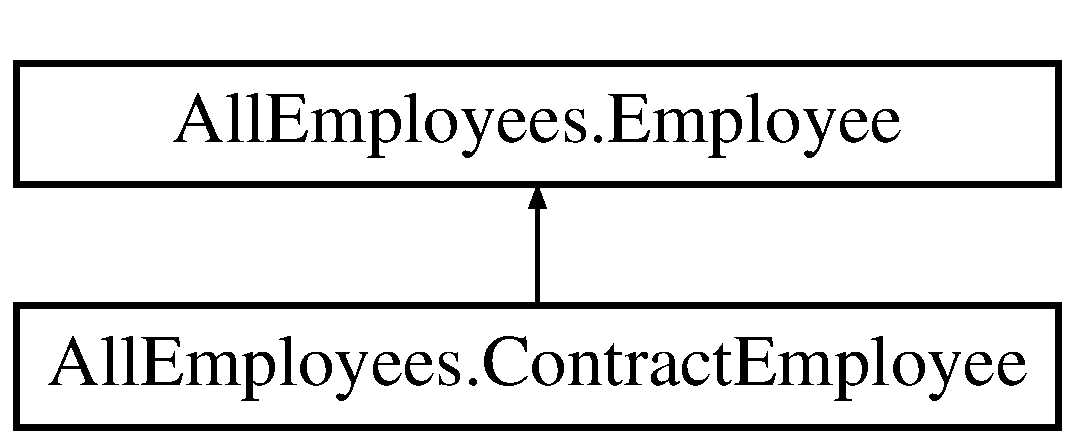
\includegraphics[height=2.000000cm]{class_all_employees_1_1_contract_employee}
\end{center}
\end{figure}
\subsection*{Public Member Functions}
\begin{DoxyCompactItemize}
\item 
\hyperlink{class_all_employees_1_1_contract_employee_afb78892e913ff2a34aed4d7b78d6c9f7}{Contract\+Employee} ()
\begin{DoxyCompactList}\small\item\em default constructor. Sets all values to default \end{DoxyCompactList}\item 
\hyperlink{class_all_employees_1_1_contract_employee_ac7aa7412d0f08a2176da6e9fc0a1ddba}{Contract\+Employee} (string first\+Name, string last\+Name)
\begin{DoxyCompactList}\small\item\em overloaded constructor. Sets name to inputed names, set all other values to default \end{DoxyCompactList}\item 
\hyperlink{class_all_employees_1_1_contract_employee_ad5a58ffe16b3b193e6024219a6b10174}{Contract\+Employee} (string first\+Name, string last\+Name, int social\+Insurance\+Number, Date\+Time date\+Of\+Birth, Date\+Time contract\+Start\+Date, Date\+Time contract\+Stop\+Date, float fixed\+Contract\+Amount)
\begin{DoxyCompactList}\small\item\em overloaded constructor. Sets all values to the values given. no default values \end{DoxyCompactList}\item 
bool \hyperlink{class_all_employees_1_1_contract_employee_a826e3f824d86fb6b4cd1c527350c5b3a}{Validate} ()
\begin{DoxyCompactList}\small\item\em Used to determine in the object contains a valid employee. \end{DoxyCompactList}\item 
string \hyperlink{class_all_employees_1_1_contract_employee_adc3a5e1e3280ac1ec77d1a0767b95c19}{Details} ()
\begin{DoxyCompactList}\small\item\em Used to create a formated string of all employee to be printed to the screen. \end{DoxyCompactList}\item 
override string \hyperlink{class_all_employees_1_1_contract_employee_ae0ba5deffac9dcf5317c91fd7d7f8816}{To\+String} ()
\begin{DoxyCompactList}\small\item\em Overriden method To\+String used to return a formated string of all data about employee. \end{DoxyCompactList}\item 
bool \hyperlink{class_all_employees_1_1_contract_employee_a012c48affde48858bda39a3cb9c802c4}{Set\+Contract\+Start\+Date} (Date\+Time date)
\begin{DoxyCompactList}\small\item\em Setter for contract\+Start\+Date from Date\+Time. \end{DoxyCompactList}\item 
bool \hyperlink{class_all_employees_1_1_contract_employee_aa10c777bc6b24385ceffaaff118e996e}{Set\+Contract\+Start\+Date} (string date)
\begin{DoxyCompactList}\small\item\em Setter for contract\+Start\+Date from String. \end{DoxyCompactList}\item 
bool \hyperlink{class_all_employees_1_1_contract_employee_af29121fe33b4f31b28eb545235a31331}{Set\+Contract\+Start\+Date} (int year, int month, int day)
\begin{DoxyCompactList}\small\item\em Setter for contract\+Start\+Date from ints. \end{DoxyCompactList}\item 
bool \hyperlink{class_all_employees_1_1_contract_employee_a60d9959aaf0368d3d951e00dc9b9276b}{Set\+Contract\+Stop\+Date} (Date\+Time date)
\begin{DoxyCompactList}\small\item\em Setter for contract\+Stop\+Date from Date\+Time. \end{DoxyCompactList}\item 
bool \hyperlink{class_all_employees_1_1_contract_employee_a5564f971606a6c44977001b3faef78d1}{Set\+Contract\+Stop\+Date} (string date)
\begin{DoxyCompactList}\small\item\em Setter for contract\+Stop\+Date from string. \end{DoxyCompactList}\item 
bool \hyperlink{class_all_employees_1_1_contract_employee_a3f7473cd491df8b2927333287b57a33d}{Set\+Contract\+Stop\+Date} (int year, int month, int day)
\begin{DoxyCompactList}\small\item\em Setter for contract\+Stop\+Date from ints. \end{DoxyCompactList}\item 
bool \hyperlink{class_all_employees_1_1_contract_employee_acf577438381bc6c56bc8f70ce0b25111}{Set\+Fixed\+Contract\+Amount} (float contract\+Amount)
\begin{DoxyCompactList}\small\item\em Setter for fixed\+Contract\+Amount. \end{DoxyCompactList}\item 
Date\+Time \hyperlink{class_all_employees_1_1_contract_employee_a270e070d2ccf2f707c9441f0ba1f2fad}{Get\+Contract\+Start\+Date} ()
\begin{DoxyCompactList}\small\item\em Getter for contract\+Start\+Date that returns Date\+Time. \end{DoxyCompactList}\item 
string \hyperlink{class_all_employees_1_1_contract_employee_a706f9a356995be719add2e1d522d1625}{Get\+Contract\+Start\+Date\+String} ()
\begin{DoxyCompactList}\small\item\em Getter for contract\+Start\+Date that returns formatted string. \end{DoxyCompactList}\item 
Date\+Time \hyperlink{class_all_employees_1_1_contract_employee_a98cacd6f03b693ba838b36c861c59b10}{Get\+Contract\+Stop\+Date} ()
\begin{DoxyCompactList}\small\item\em Getter for contract\+Stop\+Date that returns Date\+Time. \end{DoxyCompactList}\item 
string \hyperlink{class_all_employees_1_1_contract_employee_ada12137c290146af671d8e9b8db2b3fa}{Get\+Contract\+Stop\+Date\+String} ()
\begin{DoxyCompactList}\small\item\em Getter for contract\+Stop\+Date that returns formatted string. \end{DoxyCompactList}\item 
float \hyperlink{class_all_employees_1_1_contract_employee_add493d299c7d7ea7a8f8983aee2e5fa0}{Get\+Fixed\+Contract\+Amount} ()
\begin{DoxyCompactList}\small\item\em Getter for fixed\+Contract\+Amount. \end{DoxyCompactList}\end{DoxyCompactItemize}
\subsection*{Private Attributes}
\begin{DoxyCompactItemize}
\item 
\hypertarget{class_all_employees_1_1_contract_employee_aeef462cc8bd0639b674bba0632b6586b}{}Date\+Time {\bfseries contract\+Start\+Date}\label{class_all_employees_1_1_contract_employee_aeef462cc8bd0639b674bba0632b6586b}

\item 
\hypertarget{class_all_employees_1_1_contract_employee_ab549d2c8addad182fd66246c41ca73b7}{}Date\+Time {\bfseries contract\+Stop\+Date}\label{class_all_employees_1_1_contract_employee_ab549d2c8addad182fd66246c41ca73b7}

\item 
\hypertarget{class_all_employees_1_1_contract_employee_a81526f8517894ce466b70e3ffa61a8a8}{}float {\bfseries fixed\+Contract\+Amount}\label{class_all_employees_1_1_contract_employee_a81526f8517894ce466b70e3ffa61a8a8}

\end{DoxyCompactItemize}
\subsection*{Additional Inherited Members}


\subsection{Detailed Description}
{\bfseries Brief Description} The Contract \hyperlink{class_all_employees_1_1_employee}{Employee} class is used to store and manage data about a employee who is hired on a contract This class is a child to \hyperlink{class_all_employees_1_1_employee}{Employee} class. It adds the contract start and stop date and the amout the employee is payed for the contract The base classes Social Insurance Number is treated as a buisness number for this class. 

\begin{DoxyAuthor}{Author}
{\itshape Brandon} 
\end{DoxyAuthor}


\subsection{Constructor \& Destructor Documentation}
\hypertarget{class_all_employees_1_1_contract_employee_afb78892e913ff2a34aed4d7b78d6c9f7}{}\index{All\+Employees\+::\+Contract\+Employee@{All\+Employees\+::\+Contract\+Employee}!Contract\+Employee@{Contract\+Employee}}
\index{Contract\+Employee@{Contract\+Employee}!All\+Employees\+::\+Contract\+Employee@{All\+Employees\+::\+Contract\+Employee}}
\subsubsection[{Contract\+Employee}]{\setlength{\rightskip}{0pt plus 5cm}All\+Employees.\+Contract\+Employee.\+Contract\+Employee (
\begin{DoxyParamCaption}
{}
\end{DoxyParamCaption}
)}\label{class_all_employees_1_1_contract_employee_afb78892e913ff2a34aed4d7b78d6c9f7}


default constructor. Sets all values to default 

{\bfseries Details}


\begin{DoxyParams}{Parameters}
{\em n/a} & \\
\hline
\end{DoxyParams}
\begin{DoxyReturn}{Returns}
n/a 
\end{DoxyReturn}
\hypertarget{class_all_employees_1_1_contract_employee_ac7aa7412d0f08a2176da6e9fc0a1ddba}{}\index{All\+Employees\+::\+Contract\+Employee@{All\+Employees\+::\+Contract\+Employee}!Contract\+Employee@{Contract\+Employee}}
\index{Contract\+Employee@{Contract\+Employee}!All\+Employees\+::\+Contract\+Employee@{All\+Employees\+::\+Contract\+Employee}}
\subsubsection[{Contract\+Employee}]{\setlength{\rightskip}{0pt plus 5cm}All\+Employees.\+Contract\+Employee.\+Contract\+Employee (
\begin{DoxyParamCaption}
\item[{string}]{first\+Name, }
\item[{string}]{last\+Name}
\end{DoxyParamCaption}
)}\label{class_all_employees_1_1_contract_employee_ac7aa7412d0f08a2176da6e9fc0a1ddba}


overloaded constructor. Sets name to inputed names, set all other values to default 

{\bfseries Details}


\begin{DoxyParams}{Parameters}
{\em first\+Name} & -\/ {\bfseries string} -\/ First Name of employee to add to records \\
\hline
{\em last\+Name} & -\/ {\bfseries string} -\/ Last Name of employee to add to records\\
\hline
\end{DoxyParams}

\begin{DoxyExceptions}{Exceptions}
{\em $<$\+Failed\+Constructor\+Exception$>$} & -\/ If the constructor failed to create the object\\
\hline
\end{DoxyExceptions}
\begin{DoxyReturn}{Returns}
n/a 
\end{DoxyReturn}
\hypertarget{class_all_employees_1_1_contract_employee_ad5a58ffe16b3b193e6024219a6b10174}{}\index{All\+Employees\+::\+Contract\+Employee@{All\+Employees\+::\+Contract\+Employee}!Contract\+Employee@{Contract\+Employee}}
\index{Contract\+Employee@{Contract\+Employee}!All\+Employees\+::\+Contract\+Employee@{All\+Employees\+::\+Contract\+Employee}}
\subsubsection[{Contract\+Employee}]{\setlength{\rightskip}{0pt plus 5cm}All\+Employees.\+Contract\+Employee.\+Contract\+Employee (
\begin{DoxyParamCaption}
\item[{string}]{first\+Name, }
\item[{string}]{last\+Name, }
\item[{int}]{social\+Insurance\+Number, }
\item[{Date\+Time}]{date\+Of\+Birth, }
\item[{Date\+Time}]{contract\+Start\+Date, }
\item[{Date\+Time}]{contract\+Stop\+Date, }
\item[{float}]{fixed\+Contract\+Amount}
\end{DoxyParamCaption}
)}\label{class_all_employees_1_1_contract_employee_ad5a58ffe16b3b193e6024219a6b10174}


overloaded constructor. Sets all values to the values given. no default values 

{\bfseries Details}


\begin{DoxyParams}{Parameters}
{\em first\+Name} & -\/ {\bfseries string} -\/ First Name of employee to add to records \\
\hline
{\em last\+Name} & -\/ {\bfseries string} -\/ Last Name of employee to add to records \\
\hline
{\em social\+Insurance\+Number} & -\/ {\bfseries int} -\/ Social Insurance Number of employee to add to records \\
\hline
{\em date\+Of\+Birth} & -\/ {\bfseries Date\+Time} -\/ Date Of Birth of employee to add to records \\
\hline
{\em contract\+Start\+Date} & -\/ {\bfseries Date\+Time} -\/ Contract Start Date of employee contract to add to records \\
\hline
{\em contract\+Stop\+Date} & -\/ {\bfseries Date\+Time} -\/ Contract Stop Date of employee contract to add to records \\
\hline
{\em fixed\+Contract\+Amount} & -\/ {\bfseries float} -\/ Fixed Contract Amount of employee contract to add to records\\
\hline
\end{DoxyParams}

\begin{DoxyExceptions}{Exceptions}
{\em $<$\+Failed\+Constructor\+Exception$>$} & -\/ If the constructor failed to create the object\\
\hline
\end{DoxyExceptions}
\begin{DoxyReturn}{Returns}
n/a 
\end{DoxyReturn}


\subsection{Member Function Documentation}
\hypertarget{class_all_employees_1_1_contract_employee_adc3a5e1e3280ac1ec77d1a0767b95c19}{}\index{All\+Employees\+::\+Contract\+Employee@{All\+Employees\+::\+Contract\+Employee}!Details@{Details}}
\index{Details@{Details}!All\+Employees\+::\+Contract\+Employee@{All\+Employees\+::\+Contract\+Employee}}
\subsubsection[{Details}]{\setlength{\rightskip}{0pt plus 5cm}string All\+Employees.\+Contract\+Employee.\+Details (
\begin{DoxyParamCaption}
{}
\end{DoxyParamCaption}
)}\label{class_all_employees_1_1_contract_employee_adc3a5e1e3280ac1ec77d1a0767b95c19}


Used to create a formated string of all employee to be printed to the screen. 

{\bfseries Details}


\begin{DoxyParams}{Parameters}
{\em n/a} & \\
\hline
\end{DoxyParams}
\begin{DoxyReturn}{Returns}
user\+Info {\bfseries string} -\/ formatted string of employee data 
\end{DoxyReturn}
\hypertarget{class_all_employees_1_1_contract_employee_a270e070d2ccf2f707c9441f0ba1f2fad}{}\index{All\+Employees\+::\+Contract\+Employee@{All\+Employees\+::\+Contract\+Employee}!Get\+Contract\+Start\+Date@{Get\+Contract\+Start\+Date}}
\index{Get\+Contract\+Start\+Date@{Get\+Contract\+Start\+Date}!All\+Employees\+::\+Contract\+Employee@{All\+Employees\+::\+Contract\+Employee}}
\subsubsection[{Get\+Contract\+Start\+Date}]{\setlength{\rightskip}{0pt plus 5cm}Date\+Time All\+Employees.\+Contract\+Employee.\+Get\+Contract\+Start\+Date (
\begin{DoxyParamCaption}
{}
\end{DoxyParamCaption}
)}\label{class_all_employees_1_1_contract_employee_a270e070d2ccf2f707c9441f0ba1f2fad}


Getter for contract\+Start\+Date that returns Date\+Time. 

{\bfseries Details}


\begin{DoxyParams}{Parameters}
{\em n/a} & \\
\hline
\end{DoxyParams}
\begin{DoxyReturn}{Returns}
contract\+Start\+Date {\bfseries Date\+Time} 
\end{DoxyReturn}
\hypertarget{class_all_employees_1_1_contract_employee_a706f9a356995be719add2e1d522d1625}{}\index{All\+Employees\+::\+Contract\+Employee@{All\+Employees\+::\+Contract\+Employee}!Get\+Contract\+Start\+Date\+String@{Get\+Contract\+Start\+Date\+String}}
\index{Get\+Contract\+Start\+Date\+String@{Get\+Contract\+Start\+Date\+String}!All\+Employees\+::\+Contract\+Employee@{All\+Employees\+::\+Contract\+Employee}}
\subsubsection[{Get\+Contract\+Start\+Date\+String}]{\setlength{\rightskip}{0pt plus 5cm}string All\+Employees.\+Contract\+Employee.\+Get\+Contract\+Start\+Date\+String (
\begin{DoxyParamCaption}
{}
\end{DoxyParamCaption}
)}\label{class_all_employees_1_1_contract_employee_a706f9a356995be719add2e1d522d1625}


Getter for contract\+Start\+Date that returns formatted string. 

{\bfseries Details}


\begin{DoxyParams}{Parameters}
{\em n/a} & \\
\hline
\end{DoxyParams}
\begin{DoxyReturn}{Returns}
contract\+Start\+Date {\bfseries string} 
\end{DoxyReturn}
\hypertarget{class_all_employees_1_1_contract_employee_a98cacd6f03b693ba838b36c861c59b10}{}\index{All\+Employees\+::\+Contract\+Employee@{All\+Employees\+::\+Contract\+Employee}!Get\+Contract\+Stop\+Date@{Get\+Contract\+Stop\+Date}}
\index{Get\+Contract\+Stop\+Date@{Get\+Contract\+Stop\+Date}!All\+Employees\+::\+Contract\+Employee@{All\+Employees\+::\+Contract\+Employee}}
\subsubsection[{Get\+Contract\+Stop\+Date}]{\setlength{\rightskip}{0pt plus 5cm}Date\+Time All\+Employees.\+Contract\+Employee.\+Get\+Contract\+Stop\+Date (
\begin{DoxyParamCaption}
{}
\end{DoxyParamCaption}
)}\label{class_all_employees_1_1_contract_employee_a98cacd6f03b693ba838b36c861c59b10}


Getter for contract\+Stop\+Date that returns Date\+Time. 

{\bfseries Details}


\begin{DoxyParams}{Parameters}
{\em n/a} & \\
\hline
\end{DoxyParams}
\begin{DoxyReturn}{Returns}
contract\+Stop\+Date {\bfseries Date\+Time} 
\end{DoxyReturn}
\hypertarget{class_all_employees_1_1_contract_employee_ada12137c290146af671d8e9b8db2b3fa}{}\index{All\+Employees\+::\+Contract\+Employee@{All\+Employees\+::\+Contract\+Employee}!Get\+Contract\+Stop\+Date\+String@{Get\+Contract\+Stop\+Date\+String}}
\index{Get\+Contract\+Stop\+Date\+String@{Get\+Contract\+Stop\+Date\+String}!All\+Employees\+::\+Contract\+Employee@{All\+Employees\+::\+Contract\+Employee}}
\subsubsection[{Get\+Contract\+Stop\+Date\+String}]{\setlength{\rightskip}{0pt plus 5cm}string All\+Employees.\+Contract\+Employee.\+Get\+Contract\+Stop\+Date\+String (
\begin{DoxyParamCaption}
{}
\end{DoxyParamCaption}
)}\label{class_all_employees_1_1_contract_employee_ada12137c290146af671d8e9b8db2b3fa}


Getter for contract\+Stop\+Date that returns formatted string. 

{\bfseries Details}


\begin{DoxyParams}{Parameters}
{\em n/a} & \\
\hline
\end{DoxyParams}
\begin{DoxyReturn}{Returns}
contract\+Stop\+Date {\bfseries string} 
\end{DoxyReturn}
\hypertarget{class_all_employees_1_1_contract_employee_add493d299c7d7ea7a8f8983aee2e5fa0}{}\index{All\+Employees\+::\+Contract\+Employee@{All\+Employees\+::\+Contract\+Employee}!Get\+Fixed\+Contract\+Amount@{Get\+Fixed\+Contract\+Amount}}
\index{Get\+Fixed\+Contract\+Amount@{Get\+Fixed\+Contract\+Amount}!All\+Employees\+::\+Contract\+Employee@{All\+Employees\+::\+Contract\+Employee}}
\subsubsection[{Get\+Fixed\+Contract\+Amount}]{\setlength{\rightskip}{0pt plus 5cm}float All\+Employees.\+Contract\+Employee.\+Get\+Fixed\+Contract\+Amount (
\begin{DoxyParamCaption}
{}
\end{DoxyParamCaption}
)}\label{class_all_employees_1_1_contract_employee_add493d299c7d7ea7a8f8983aee2e5fa0}


Getter for fixed\+Contract\+Amount. 

{\bfseries Details}


\begin{DoxyParams}{Parameters}
{\em n/a} & \\
\hline
\end{DoxyParams}
\begin{DoxyReturn}{Returns}
fixed\+Contract\+Amount {\bfseries float} 
\end{DoxyReturn}
\hypertarget{class_all_employees_1_1_contract_employee_a012c48affde48858bda39a3cb9c802c4}{}\index{All\+Employees\+::\+Contract\+Employee@{All\+Employees\+::\+Contract\+Employee}!Set\+Contract\+Start\+Date@{Set\+Contract\+Start\+Date}}
\index{Set\+Contract\+Start\+Date@{Set\+Contract\+Start\+Date}!All\+Employees\+::\+Contract\+Employee@{All\+Employees\+::\+Contract\+Employee}}
\subsubsection[{Set\+Contract\+Start\+Date}]{\setlength{\rightskip}{0pt plus 5cm}bool All\+Employees.\+Contract\+Employee.\+Set\+Contract\+Start\+Date (
\begin{DoxyParamCaption}
\item[{Date\+Time}]{date}
\end{DoxyParamCaption}
)}\label{class_all_employees_1_1_contract_employee_a012c48affde48858bda39a3cb9c802c4}


Setter for contract\+Start\+Date from Date\+Time. 

{\bfseries Details}


\begin{DoxyParams}{Parameters}
{\em date} & {\bfseries Date\+Time} -\/ The start date of the employees contract\\
\hline
\end{DoxyParams}
\begin{DoxyReturn}{Returns}
data\+Saved {\bfseries bool} -\/ true if input was valid and data was changed. False it data was not changed 
\end{DoxyReturn}
\hypertarget{class_all_employees_1_1_contract_employee_aa10c777bc6b24385ceffaaff118e996e}{}\index{All\+Employees\+::\+Contract\+Employee@{All\+Employees\+::\+Contract\+Employee}!Set\+Contract\+Start\+Date@{Set\+Contract\+Start\+Date}}
\index{Set\+Contract\+Start\+Date@{Set\+Contract\+Start\+Date}!All\+Employees\+::\+Contract\+Employee@{All\+Employees\+::\+Contract\+Employee}}
\subsubsection[{Set\+Contract\+Start\+Date}]{\setlength{\rightskip}{0pt plus 5cm}bool All\+Employees.\+Contract\+Employee.\+Set\+Contract\+Start\+Date (
\begin{DoxyParamCaption}
\item[{string}]{date}
\end{DoxyParamCaption}
)}\label{class_all_employees_1_1_contract_employee_aa10c777bc6b24385ceffaaff118e996e}


Setter for contract\+Start\+Date from String. 

{\bfseries Details}


\begin{DoxyParams}{Parameters}
{\em date} & {\bfseries string} -\/ The start date of the employees contract\\
\hline
\end{DoxyParams}
\begin{DoxyReturn}{Returns}
data\+Saved {\bfseries bool} -\/ true if input was valid and data was changed. False it data was not changed 
\end{DoxyReturn}
\hypertarget{class_all_employees_1_1_contract_employee_af29121fe33b4f31b28eb545235a31331}{}\index{All\+Employees\+::\+Contract\+Employee@{All\+Employees\+::\+Contract\+Employee}!Set\+Contract\+Start\+Date@{Set\+Contract\+Start\+Date}}
\index{Set\+Contract\+Start\+Date@{Set\+Contract\+Start\+Date}!All\+Employees\+::\+Contract\+Employee@{All\+Employees\+::\+Contract\+Employee}}
\subsubsection[{Set\+Contract\+Start\+Date}]{\setlength{\rightskip}{0pt plus 5cm}bool All\+Employees.\+Contract\+Employee.\+Set\+Contract\+Start\+Date (
\begin{DoxyParamCaption}
\item[{int}]{year, }
\item[{int}]{month, }
\item[{int}]{day}
\end{DoxyParamCaption}
)}\label{class_all_employees_1_1_contract_employee_af29121fe33b4f31b28eb545235a31331}


Setter for contract\+Start\+Date from ints. 

{\bfseries Details}


\begin{DoxyParams}{Parameters}
{\em year} & {\bfseries int} -\/ The start year of the employees contract \\
\hline
{\em month} & {\bfseries int} -\/ The start month of the employees contract \\
\hline
{\em day} & {\bfseries int} -\/ The start day of the employees contract\\
\hline
\end{DoxyParams}
\begin{DoxyReturn}{Returns}
data\+Saved {\bfseries bool} -\/ true if input was valid and data was changed. False it data was not changed 
\end{DoxyReturn}
\hypertarget{class_all_employees_1_1_contract_employee_a60d9959aaf0368d3d951e00dc9b9276b}{}\index{All\+Employees\+::\+Contract\+Employee@{All\+Employees\+::\+Contract\+Employee}!Set\+Contract\+Stop\+Date@{Set\+Contract\+Stop\+Date}}
\index{Set\+Contract\+Stop\+Date@{Set\+Contract\+Stop\+Date}!All\+Employees\+::\+Contract\+Employee@{All\+Employees\+::\+Contract\+Employee}}
\subsubsection[{Set\+Contract\+Stop\+Date}]{\setlength{\rightskip}{0pt plus 5cm}bool All\+Employees.\+Contract\+Employee.\+Set\+Contract\+Stop\+Date (
\begin{DoxyParamCaption}
\item[{Date\+Time}]{date}
\end{DoxyParamCaption}
)}\label{class_all_employees_1_1_contract_employee_a60d9959aaf0368d3d951e00dc9b9276b}


Setter for contract\+Stop\+Date from Date\+Time. 

{\bfseries Details}


\begin{DoxyParams}{Parameters}
{\em date} & {\bfseries Date\+Time} -\/ The stop date of the employees contract\\
\hline
\end{DoxyParams}
\begin{DoxyReturn}{Returns}
data\+Saved {\bfseries bool} -\/ true if input was valid and data was changed. False it data was not changed 
\end{DoxyReturn}
\hypertarget{class_all_employees_1_1_contract_employee_a5564f971606a6c44977001b3faef78d1}{}\index{All\+Employees\+::\+Contract\+Employee@{All\+Employees\+::\+Contract\+Employee}!Set\+Contract\+Stop\+Date@{Set\+Contract\+Stop\+Date}}
\index{Set\+Contract\+Stop\+Date@{Set\+Contract\+Stop\+Date}!All\+Employees\+::\+Contract\+Employee@{All\+Employees\+::\+Contract\+Employee}}
\subsubsection[{Set\+Contract\+Stop\+Date}]{\setlength{\rightskip}{0pt plus 5cm}bool All\+Employees.\+Contract\+Employee.\+Set\+Contract\+Stop\+Date (
\begin{DoxyParamCaption}
\item[{string}]{date}
\end{DoxyParamCaption}
)}\label{class_all_employees_1_1_contract_employee_a5564f971606a6c44977001b3faef78d1}


Setter for contract\+Stop\+Date from string. 

{\bfseries Details}


\begin{DoxyParams}{Parameters}
{\em date} & {\bfseries string} -\/ The stop date of the employees contract\\
\hline
\end{DoxyParams}
\begin{DoxyReturn}{Returns}
data\+Saved {\bfseries bool} -\/ true if input was valid and data was changed. False it data was not changed 
\end{DoxyReturn}
\hypertarget{class_all_employees_1_1_contract_employee_a3f7473cd491df8b2927333287b57a33d}{}\index{All\+Employees\+::\+Contract\+Employee@{All\+Employees\+::\+Contract\+Employee}!Set\+Contract\+Stop\+Date@{Set\+Contract\+Stop\+Date}}
\index{Set\+Contract\+Stop\+Date@{Set\+Contract\+Stop\+Date}!All\+Employees\+::\+Contract\+Employee@{All\+Employees\+::\+Contract\+Employee}}
\subsubsection[{Set\+Contract\+Stop\+Date}]{\setlength{\rightskip}{0pt plus 5cm}bool All\+Employees.\+Contract\+Employee.\+Set\+Contract\+Stop\+Date (
\begin{DoxyParamCaption}
\item[{int}]{year, }
\item[{int}]{month, }
\item[{int}]{day}
\end{DoxyParamCaption}
)}\label{class_all_employees_1_1_contract_employee_a3f7473cd491df8b2927333287b57a33d}


Setter for contract\+Stop\+Date from ints. 

{\bfseries Details}


\begin{DoxyParams}{Parameters}
{\em year} & {\bfseries int} -\/ The stop year of the employees contract \\
\hline
{\em month} & {\bfseries int} -\/ The stop month of the employees contract \\
\hline
{\em day} & {\bfseries int} -\/ The stop day of the employees contract\\
\hline
\end{DoxyParams}
\begin{DoxyReturn}{Returns}
data\+Saved {\bfseries bool} -\/ true if input was valid and data was changed. False it data was not changed 
\end{DoxyReturn}
\hypertarget{class_all_employees_1_1_contract_employee_acf577438381bc6c56bc8f70ce0b25111}{}\index{All\+Employees\+::\+Contract\+Employee@{All\+Employees\+::\+Contract\+Employee}!Set\+Fixed\+Contract\+Amount@{Set\+Fixed\+Contract\+Amount}}
\index{Set\+Fixed\+Contract\+Amount@{Set\+Fixed\+Contract\+Amount}!All\+Employees\+::\+Contract\+Employee@{All\+Employees\+::\+Contract\+Employee}}
\subsubsection[{Set\+Fixed\+Contract\+Amount}]{\setlength{\rightskip}{0pt plus 5cm}bool All\+Employees.\+Contract\+Employee.\+Set\+Fixed\+Contract\+Amount (
\begin{DoxyParamCaption}
\item[{float}]{contract\+Amount}
\end{DoxyParamCaption}
)}\label{class_all_employees_1_1_contract_employee_acf577438381bc6c56bc8f70ce0b25111}


Setter for fixed\+Contract\+Amount. 

{\bfseries Details}


\begin{DoxyParams}{Parameters}
{\em contract\+Amount} & {\bfseries float} -\/ The amount the contract is payed\\
\hline
\end{DoxyParams}
\begin{DoxyReturn}{Returns}
data\+Saves {\bfseries bool} -\/ true if input was valid and data was changed. False it data was not changed 
\end{DoxyReturn}
\hypertarget{class_all_employees_1_1_contract_employee_ae0ba5deffac9dcf5317c91fd7d7f8816}{}\index{All\+Employees\+::\+Contract\+Employee@{All\+Employees\+::\+Contract\+Employee}!To\+String@{To\+String}}
\index{To\+String@{To\+String}!All\+Employees\+::\+Contract\+Employee@{All\+Employees\+::\+Contract\+Employee}}
\subsubsection[{To\+String}]{\setlength{\rightskip}{0pt plus 5cm}override string All\+Employees.\+Contract\+Employee.\+To\+String (
\begin{DoxyParamCaption}
{}
\end{DoxyParamCaption}
)}\label{class_all_employees_1_1_contract_employee_ae0ba5deffac9dcf5317c91fd7d7f8816}


Overriden method To\+String used to return a formated string of all data about employee. 

{\bfseries Details}


\begin{DoxyParams}{Parameters}
{\em n/a} & \\
\hline
\end{DoxyParams}
\begin{DoxyReturn}{Returns}
employee\+String {\bfseries string} -\/ the formated string containing all employee data 
\end{DoxyReturn}
\hypertarget{class_all_employees_1_1_contract_employee_a826e3f824d86fb6b4cd1c527350c5b3a}{}\index{All\+Employees\+::\+Contract\+Employee@{All\+Employees\+::\+Contract\+Employee}!Validate@{Validate}}
\index{Validate@{Validate}!All\+Employees\+::\+Contract\+Employee@{All\+Employees\+::\+Contract\+Employee}}
\subsubsection[{Validate}]{\setlength{\rightskip}{0pt plus 5cm}bool All\+Employees.\+Contract\+Employee.\+Validate (
\begin{DoxyParamCaption}
{}
\end{DoxyParamCaption}
)}\label{class_all_employees_1_1_contract_employee_a826e3f824d86fb6b4cd1c527350c5b3a}


Used to determine in the object contains a valid employee. 

{\bfseries Details}


\begin{DoxyParams}{Parameters}
{\em n/a} & \\
\hline
\end{DoxyParams}
\begin{DoxyReturn}{Returns}
data\+Valid -\/ {\bfseries bool} -\/ True if the object contains all data for a valid employee 
\end{DoxyReturn}


The documentation for this class was generated from the following file\+:\begin{DoxyCompactItemize}
\item 
C\+:/\+S\+E\+T\+Repo/trunk/\+E\+M\+S/trunk/\+All\+Employees/\+All\+Employees/Contract\+Employee.\+cs\end{DoxyCompactItemize}

\hypertarget{class_all_employees_1_1_employee}{}\section{All\+Employees.\+Employee Class Reference}
\label{class_all_employees_1_1_employee}\index{All\+Employees.\+Employee@{All\+Employees.\+Employee}}


{\bfseries Brief Description} The \hyperlink{class_all_employees_1_1_employee}{Employee} class is used to hold the basic infomation for all types of employees This class is the parent to many classes that furthur define different types of employees  


Inheritance diagram for All\+Employees.\+Employee\+:\begin{figure}[H]
\begin{center}
\leavevmode
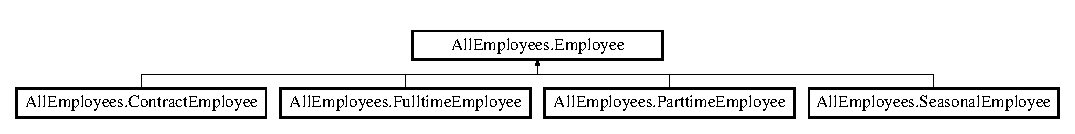
\includegraphics[height=1.352657cm]{class_all_employees_1_1_employee}
\end{center}
\end{figure}
\subsection*{Public Member Functions}
\begin{DoxyCompactItemize}
\item 
\hyperlink{class_all_employees_1_1_employee_ac3aa5a59bf1ddba2c45cc933bf897e04}{Employee} ()
\begin{DoxyCompactList}\small\item\em default constructor. Sets all values to default \end{DoxyCompactList}\item 
\hyperlink{class_all_employees_1_1_employee_a0a75e7e1786f2c6e5fa482ad79a99234}{Employee} (string first\+Name, string last\+Name)
\begin{DoxyCompactList}\small\item\em overloaded constructor. Sets name to inputed names, set all other values to default \end{DoxyCompactList}\item 
\hyperlink{class_all_employees_1_1_employee_aae0bb0d49eb93ff488771dca5a3db315}{Employee} (string first\+Name, string last\+Name, int social\+Insurance\+Number, Date\+Time date\+Of\+Birth, string employee\+Type)
\begin{DoxyCompactList}\small\item\em overloaded constructor. Sets all values to the values given. no default values \end{DoxyCompactList}\item 
bool \hyperlink{class_all_employees_1_1_employee_ad44ba8da1da1dceb64e1e6f9e6f7c5a3}{Set\+First\+Name} (string first\+Name)
\begin{DoxyCompactList}\small\item\em Setter for first\+Name. \end{DoxyCompactList}\item 
bool \hyperlink{class_all_employees_1_1_employee_a2b5ead1b4de39d2024422c4443034d4c}{Set\+Last\+Name} (string last\+Name)
\begin{DoxyCompactList}\small\item\em Setter for last\+Name. \end{DoxyCompactList}\item 
bool \hyperlink{class_all_employees_1_1_employee_a25c3c9fd99a595fb812b3ba6791f3f11}{Set\+Social\+Insurance\+Number} (int social\+Insurance\+Number)
\begin{DoxyCompactList}\small\item\em Setter for social\+Insurance\+Number. \end{DoxyCompactList}\item 
bool \hyperlink{class_all_employees_1_1_employee_a058b085f3c60bbe744bd10cc1f7a2bdb}{Set\+Date\+Of\+Birth} (Date\+Time date)
\begin{DoxyCompactList}\small\item\em Setter for date\+Of\+Birth using Date\+Time. \end{DoxyCompactList}\item 
bool \hyperlink{class_all_employees_1_1_employee_a66c163e386a335040a33a583d9d20d7c}{Set\+Date\+Of\+Birth} (string date)
\begin{DoxyCompactList}\small\item\em Setter for date\+Of\+Birth with String. \end{DoxyCompactList}\item 
bool \hyperlink{class_all_employees_1_1_employee_ac095c524a6b57edd0daea893c89874f5}{Set\+Date\+Of\+Birth} (int year, int month, int day)
\begin{DoxyCompactList}\small\item\em Setter for date\+Of\+Birth with ints. \end{DoxyCompactList}\item 
bool \hyperlink{class_all_employees_1_1_employee_aabdb35f9e42e4847bc33fda68482f7ab}{Set\+Employee\+Type} (string employee\+Type)
\begin{DoxyCompactList}\small\item\em Setter for type of employee. \end{DoxyCompactList}\item 
string \hyperlink{class_all_employees_1_1_employee_ae585e71d63222bcd0b87581fc8c1f936}{Get\+First\+Name} ()
\begin{DoxyCompactList}\small\item\em Getter for first\+Name. \end{DoxyCompactList}\item 
string \hyperlink{class_all_employees_1_1_employee_afaf5dbaa12c35930b36d3582e831b407}{Get\+Last\+Name} ()
\begin{DoxyCompactList}\small\item\em Getter for last\+Name. \end{DoxyCompactList}\item 
int \hyperlink{class_all_employees_1_1_employee_a0b5c62bd8eca3acd7f0921a478d8aefa}{Get\+Social\+Insurance\+Number} ()
\begin{DoxyCompactList}\small\item\em Getter for social\+Insurance\+Number. \end{DoxyCompactList}\item 
Date\+Time \hyperlink{class_all_employees_1_1_employee_a98f7200d68ab6a59f4e3283b8f81ce28}{Get\+Date\+Of\+Birth} ()
\begin{DoxyCompactList}\small\item\em Getter for date\+Of\+Birth. \end{DoxyCompactList}\item 
string \hyperlink{class_all_employees_1_1_employee_a2c310cf42cb87541a5fde6771e667212}{Get\+Date\+Of\+Birth\+String} ()
\begin{DoxyCompactList}\small\item\em Getter for date\+Of\+Birth that returns formatted string. \end{DoxyCompactList}\item 
string \hyperlink{class_all_employees_1_1_employee_a39116fe8a1dcc18735c92c1a3fcb579e}{Get\+Employee\+Type} ()
\begin{DoxyCompactList}\small\item\em Getter for employee\+Type. \end{DoxyCompactList}\end{DoxyCompactItemize}
\subsection*{Protected Member Functions}
\begin{DoxyCompactItemize}
\item 
bool \hyperlink{class_all_employees_1_1_employee_af679e8b4c683b9e94bec085062e5c88e}{Validate\+Base} ()
\begin{DoxyCompactList}\small\item\em Used to determine in the object contains a valid employee. \end{DoxyCompactList}\item 
string \hyperlink{class_all_employees_1_1_employee_a9e957826e327579e190cd5075789d1a9}{To\+String\+Base} ()
\begin{DoxyCompactList}\small\item\em Overriden method To\+String used to return a formated string of all data. \end{DoxyCompactList}\end{DoxyCompactItemize}
\subsection*{Private Attributes}
\begin{DoxyCompactItemize}
\item 
\hypertarget{class_all_employees_1_1_employee_a04c4c16015aa2d889fd2042ce4b8a1d7}{}string {\bfseries first\+Name}\label{class_all_employees_1_1_employee_a04c4c16015aa2d889fd2042ce4b8a1d7}

\item 
\hypertarget{class_all_employees_1_1_employee_ac3721b61919ca9cd29a400620562170e}{}string {\bfseries last\+Name}\label{class_all_employees_1_1_employee_ac3721b61919ca9cd29a400620562170e}

\item 
\hypertarget{class_all_employees_1_1_employee_a31f55bb91fe0871c5d9a3cb77f44a4df}{}int {\bfseries social\+Insurance\+Number}\label{class_all_employees_1_1_employee_a31f55bb91fe0871c5d9a3cb77f44a4df}

\item 
\hypertarget{class_all_employees_1_1_employee_a00f33298e4408f0a0402a34c9aa2067a}{}Date\+Time {\bfseries date\+Of\+Birth}\label{class_all_employees_1_1_employee_a00f33298e4408f0a0402a34c9aa2067a}

\item 
\hypertarget{class_all_employees_1_1_employee_a246198254823dc5a10197029b17479b4}{}string {\bfseries employee\+Type}\label{class_all_employees_1_1_employee_a246198254823dc5a10197029b17479b4}

\end{DoxyCompactItemize}


\subsection{Detailed Description}
{\bfseries Brief Description} The \hyperlink{class_all_employees_1_1_employee}{Employee} class is used to hold the basic infomation for all types of employees This class is the parent to many classes that furthur define different types of employees 

\begin{DoxyAuthor}{Author}
{\itshape Brandon} 
\end{DoxyAuthor}


\subsection{Constructor \& Destructor Documentation}
\hypertarget{class_all_employees_1_1_employee_ac3aa5a59bf1ddba2c45cc933bf897e04}{}\index{All\+Employees\+::\+Employee@{All\+Employees\+::\+Employee}!Employee@{Employee}}
\index{Employee@{Employee}!All\+Employees\+::\+Employee@{All\+Employees\+::\+Employee}}
\subsubsection[{Employee}]{\setlength{\rightskip}{0pt plus 5cm}All\+Employees.\+Employee.\+Employee (
\begin{DoxyParamCaption}
{}
\end{DoxyParamCaption}
)}\label{class_all_employees_1_1_employee_ac3aa5a59bf1ddba2c45cc933bf897e04}


default constructor. Sets all values to default 

{\bfseries Details}


\begin{DoxyParams}{Parameters}
{\em n/a} & \\
\hline
\end{DoxyParams}
\begin{DoxyReturn}{Returns}
n/a 
\end{DoxyReturn}
\hypertarget{class_all_employees_1_1_employee_a0a75e7e1786f2c6e5fa482ad79a99234}{}\index{All\+Employees\+::\+Employee@{All\+Employees\+::\+Employee}!Employee@{Employee}}
\index{Employee@{Employee}!All\+Employees\+::\+Employee@{All\+Employees\+::\+Employee}}
\subsubsection[{Employee}]{\setlength{\rightskip}{0pt plus 5cm}All\+Employees.\+Employee.\+Employee (
\begin{DoxyParamCaption}
\item[{string}]{first\+Name, }
\item[{string}]{last\+Name}
\end{DoxyParamCaption}
)}\label{class_all_employees_1_1_employee_a0a75e7e1786f2c6e5fa482ad79a99234}


overloaded constructor. Sets name to inputed names, set all other values to default 

{\bfseries Details}


\begin{DoxyParams}{Parameters}
{\em first\+Name} & -\/ {\bfseries string} -\/ First Name of employee to add to records \\
\hline
{\em last\+Name} & -\/ {\bfseries string} -\/ Last Name of employee to add to records\\
\hline
\end{DoxyParams}

\begin{DoxyExceptions}{Exceptions}
{\em $<$\+Failed\+Constructor\+Exception$>$} & -\/ If the constructor failed to create the object\\
\hline
\end{DoxyExceptions}
\begin{DoxyReturn}{Returns}
n/a 
\end{DoxyReturn}
\hypertarget{class_all_employees_1_1_employee_aae0bb0d49eb93ff488771dca5a3db315}{}\index{All\+Employees\+::\+Employee@{All\+Employees\+::\+Employee}!Employee@{Employee}}
\index{Employee@{Employee}!All\+Employees\+::\+Employee@{All\+Employees\+::\+Employee}}
\subsubsection[{Employee}]{\setlength{\rightskip}{0pt plus 5cm}All\+Employees.\+Employee.\+Employee (
\begin{DoxyParamCaption}
\item[{string}]{first\+Name, }
\item[{string}]{last\+Name, }
\item[{int}]{social\+Insurance\+Number, }
\item[{Date\+Time}]{date\+Of\+Birth, }
\item[{string}]{employee\+Type}
\end{DoxyParamCaption}
)}\label{class_all_employees_1_1_employee_aae0bb0d49eb93ff488771dca5a3db315}


overloaded constructor. Sets all values to the values given. no default values 

{\bfseries Details}


\begin{DoxyParams}{Parameters}
{\em first\+Name} & -\/ {\bfseries string} -\/ First Name of employee to add to records \\
\hline
{\em last\+Name} & -\/ {\bfseries string} -\/ Last Name of employee to add to records \\
\hline
{\em social\+Insurance\+Number} & -\/ {\bfseries int} -\/ Social Insurance Number of employee to add to records \\
\hline
{\em date\+Of\+Birth} & -\/ {\bfseries Date\+Time} -\/ Date Of Birth of employee to add to records\\
\hline
\end{DoxyParams}

\begin{DoxyExceptions}{Exceptions}
{\em $<$\+Failed\+Constructor\+Exception$>$} & -\/ If the constructor failed to create the object\\
\hline
\end{DoxyExceptions}
\begin{DoxyReturn}{Returns}
n/a 
\end{DoxyReturn}


\subsection{Member Function Documentation}
\hypertarget{class_all_employees_1_1_employee_a98f7200d68ab6a59f4e3283b8f81ce28}{}\index{All\+Employees\+::\+Employee@{All\+Employees\+::\+Employee}!Get\+Date\+Of\+Birth@{Get\+Date\+Of\+Birth}}
\index{Get\+Date\+Of\+Birth@{Get\+Date\+Of\+Birth}!All\+Employees\+::\+Employee@{All\+Employees\+::\+Employee}}
\subsubsection[{Get\+Date\+Of\+Birth}]{\setlength{\rightskip}{0pt plus 5cm}Date\+Time All\+Employees.\+Employee.\+Get\+Date\+Of\+Birth (
\begin{DoxyParamCaption}
{}
\end{DoxyParamCaption}
)}\label{class_all_employees_1_1_employee_a98f7200d68ab6a59f4e3283b8f81ce28}


Getter for date\+Of\+Birth. 

{\bfseries Details}


\begin{DoxyParams}{Parameters}
{\em n/a} & \\
\hline
\end{DoxyParams}
\begin{DoxyReturn}{Returns}
date\+Of\+Birth {\bfseries string} 
\end{DoxyReturn}
\hypertarget{class_all_employees_1_1_employee_a2c310cf42cb87541a5fde6771e667212}{}\index{All\+Employees\+::\+Employee@{All\+Employees\+::\+Employee}!Get\+Date\+Of\+Birth\+String@{Get\+Date\+Of\+Birth\+String}}
\index{Get\+Date\+Of\+Birth\+String@{Get\+Date\+Of\+Birth\+String}!All\+Employees\+::\+Employee@{All\+Employees\+::\+Employee}}
\subsubsection[{Get\+Date\+Of\+Birth\+String}]{\setlength{\rightskip}{0pt plus 5cm}string All\+Employees.\+Employee.\+Get\+Date\+Of\+Birth\+String (
\begin{DoxyParamCaption}
{}
\end{DoxyParamCaption}
)}\label{class_all_employees_1_1_employee_a2c310cf42cb87541a5fde6771e667212}


Getter for date\+Of\+Birth that returns formatted string. 

{\bfseries Details}


\begin{DoxyParams}{Parameters}
{\em n/a} & \\
\hline
\end{DoxyParams}
\begin{DoxyReturn}{Returns}
date\+Of\+Birth {\bfseries string} 
\end{DoxyReturn}
\hypertarget{class_all_employees_1_1_employee_a39116fe8a1dcc18735c92c1a3fcb579e}{}\index{All\+Employees\+::\+Employee@{All\+Employees\+::\+Employee}!Get\+Employee\+Type@{Get\+Employee\+Type}}
\index{Get\+Employee\+Type@{Get\+Employee\+Type}!All\+Employees\+::\+Employee@{All\+Employees\+::\+Employee}}
\subsubsection[{Get\+Employee\+Type}]{\setlength{\rightskip}{0pt plus 5cm}string All\+Employees.\+Employee.\+Get\+Employee\+Type (
\begin{DoxyParamCaption}
{}
\end{DoxyParamCaption}
)}\label{class_all_employees_1_1_employee_a39116fe8a1dcc18735c92c1a3fcb579e}


Getter for employee\+Type. 

{\bfseries Details}


\begin{DoxyParams}{Parameters}
{\em n/a} & \\
\hline
\end{DoxyParams}
\begin{DoxyReturn}{Returns}
employee\+Type {\bfseries string} 
\end{DoxyReturn}
\hypertarget{class_all_employees_1_1_employee_ae585e71d63222bcd0b87581fc8c1f936}{}\index{All\+Employees\+::\+Employee@{All\+Employees\+::\+Employee}!Get\+First\+Name@{Get\+First\+Name}}
\index{Get\+First\+Name@{Get\+First\+Name}!All\+Employees\+::\+Employee@{All\+Employees\+::\+Employee}}
\subsubsection[{Get\+First\+Name}]{\setlength{\rightskip}{0pt plus 5cm}string All\+Employees.\+Employee.\+Get\+First\+Name (
\begin{DoxyParamCaption}
{}
\end{DoxyParamCaption}
)}\label{class_all_employees_1_1_employee_ae585e71d63222bcd0b87581fc8c1f936}


Getter for first\+Name. 

{\bfseries Details}


\begin{DoxyParams}{Parameters}
{\em n/a} & \\
\hline
\end{DoxyParams}
\begin{DoxyReturn}{Returns}
first\+Name {\bfseries string} 
\end{DoxyReturn}
\hypertarget{class_all_employees_1_1_employee_afaf5dbaa12c35930b36d3582e831b407}{}\index{All\+Employees\+::\+Employee@{All\+Employees\+::\+Employee}!Get\+Last\+Name@{Get\+Last\+Name}}
\index{Get\+Last\+Name@{Get\+Last\+Name}!All\+Employees\+::\+Employee@{All\+Employees\+::\+Employee}}
\subsubsection[{Get\+Last\+Name}]{\setlength{\rightskip}{0pt plus 5cm}string All\+Employees.\+Employee.\+Get\+Last\+Name (
\begin{DoxyParamCaption}
{}
\end{DoxyParamCaption}
)}\label{class_all_employees_1_1_employee_afaf5dbaa12c35930b36d3582e831b407}


Getter for last\+Name. 

{\bfseries Details}


\begin{DoxyParams}{Parameters}
{\em n/a} & \\
\hline
\end{DoxyParams}
\begin{DoxyReturn}{Returns}
last\+Name {\bfseries string} 
\end{DoxyReturn}
\hypertarget{class_all_employees_1_1_employee_a0b5c62bd8eca3acd7f0921a478d8aefa}{}\index{All\+Employees\+::\+Employee@{All\+Employees\+::\+Employee}!Get\+Social\+Insurance\+Number@{Get\+Social\+Insurance\+Number}}
\index{Get\+Social\+Insurance\+Number@{Get\+Social\+Insurance\+Number}!All\+Employees\+::\+Employee@{All\+Employees\+::\+Employee}}
\subsubsection[{Get\+Social\+Insurance\+Number}]{\setlength{\rightskip}{0pt plus 5cm}int All\+Employees.\+Employee.\+Get\+Social\+Insurance\+Number (
\begin{DoxyParamCaption}
{}
\end{DoxyParamCaption}
)}\label{class_all_employees_1_1_employee_a0b5c62bd8eca3acd7f0921a478d8aefa}


Getter for social\+Insurance\+Number. 

{\bfseries Details}


\begin{DoxyParams}{Parameters}
{\em n/a} & \\
\hline
\end{DoxyParams}
\begin{DoxyReturn}{Returns}
social\+Insurance\+Number {\bfseries int} 
\end{DoxyReturn}
\hypertarget{class_all_employees_1_1_employee_a058b085f3c60bbe744bd10cc1f7a2bdb}{}\index{All\+Employees\+::\+Employee@{All\+Employees\+::\+Employee}!Set\+Date\+Of\+Birth@{Set\+Date\+Of\+Birth}}
\index{Set\+Date\+Of\+Birth@{Set\+Date\+Of\+Birth}!All\+Employees\+::\+Employee@{All\+Employees\+::\+Employee}}
\subsubsection[{Set\+Date\+Of\+Birth}]{\setlength{\rightskip}{0pt plus 5cm}bool All\+Employees.\+Employee.\+Set\+Date\+Of\+Birth (
\begin{DoxyParamCaption}
\item[{Date\+Time}]{date}
\end{DoxyParamCaption}
)}\label{class_all_employees_1_1_employee_a058b085f3c60bbe744bd10cc1f7a2bdb}


Setter for date\+Of\+Birth using Date\+Time. 

{\bfseries Details}


\begin{DoxyParams}{Parameters}
{\em date} & {\bfseries Date\+Time} -\/ The date of birth of the employee\\
\hline
\end{DoxyParams}
\begin{DoxyReturn}{Returns}
data\+Saved {\bfseries bool} -\/ true if input was valid and data was changed. False it data was not changed 
\end{DoxyReturn}
\hypertarget{class_all_employees_1_1_employee_a66c163e386a335040a33a583d9d20d7c}{}\index{All\+Employees\+::\+Employee@{All\+Employees\+::\+Employee}!Set\+Date\+Of\+Birth@{Set\+Date\+Of\+Birth}}
\index{Set\+Date\+Of\+Birth@{Set\+Date\+Of\+Birth}!All\+Employees\+::\+Employee@{All\+Employees\+::\+Employee}}
\subsubsection[{Set\+Date\+Of\+Birth}]{\setlength{\rightskip}{0pt plus 5cm}bool All\+Employees.\+Employee.\+Set\+Date\+Of\+Birth (
\begin{DoxyParamCaption}
\item[{string}]{date}
\end{DoxyParamCaption}
)}\label{class_all_employees_1_1_employee_a66c163e386a335040a33a583d9d20d7c}


Setter for date\+Of\+Birth with String. 

{\bfseries Details}


\begin{DoxyParams}{Parameters}
{\em date} & {\bfseries string} -\/ The date of birth of the employee\\
\hline
\end{DoxyParams}
\begin{DoxyReturn}{Returns}
data\+Saved {\bfseries bool} -\/ true if input was valid and data was changed. False it data was not changed 
\end{DoxyReturn}
\hypertarget{class_all_employees_1_1_employee_ac095c524a6b57edd0daea893c89874f5}{}\index{All\+Employees\+::\+Employee@{All\+Employees\+::\+Employee}!Set\+Date\+Of\+Birth@{Set\+Date\+Of\+Birth}}
\index{Set\+Date\+Of\+Birth@{Set\+Date\+Of\+Birth}!All\+Employees\+::\+Employee@{All\+Employees\+::\+Employee}}
\subsubsection[{Set\+Date\+Of\+Birth}]{\setlength{\rightskip}{0pt plus 5cm}bool All\+Employees.\+Employee.\+Set\+Date\+Of\+Birth (
\begin{DoxyParamCaption}
\item[{int}]{year, }
\item[{int}]{month, }
\item[{int}]{day}
\end{DoxyParamCaption}
)}\label{class_all_employees_1_1_employee_ac095c524a6b57edd0daea893c89874f5}


Setter for date\+Of\+Birth with ints. 

{\bfseries Details}


\begin{DoxyParams}{Parameters}
{\em year} & {\bfseries int} -\/ The year of birth of the employee \\
\hline
{\em month} & {\bfseries int} -\/ The month of birth of the employee \\
\hline
{\em day} & {\bfseries int} -\/ The day of birth of the employee\\
\hline
\end{DoxyParams}
\begin{DoxyReturn}{Returns}
data\+Saved {\bfseries bool} -\/ true if input was valid and data was changed. False it data was not changed 
\end{DoxyReturn}
\hypertarget{class_all_employees_1_1_employee_aabdb35f9e42e4847bc33fda68482f7ab}{}\index{All\+Employees\+::\+Employee@{All\+Employees\+::\+Employee}!Set\+Employee\+Type@{Set\+Employee\+Type}}
\index{Set\+Employee\+Type@{Set\+Employee\+Type}!All\+Employees\+::\+Employee@{All\+Employees\+::\+Employee}}
\subsubsection[{Set\+Employee\+Type}]{\setlength{\rightskip}{0pt plus 5cm}bool All\+Employees.\+Employee.\+Set\+Employee\+Type (
\begin{DoxyParamCaption}
\item[{string}]{employee\+Type}
\end{DoxyParamCaption}
)}\label{class_all_employees_1_1_employee_aabdb35f9e42e4847bc33fda68482f7ab}


Setter for type of employee. 

{\bfseries Details}


\begin{DoxyParams}{Parameters}
{\em employee\+Type} & {\bfseries string} -\/ The type of the employee. Must be\+: \char`\"{}\+F\+T\char`\"{} \char`\"{}\+P\+T\char`\"{} \char`\"{}\+C\+T\char`\"{} \char`\"{}\+S\+N\char`\"{} or \char`\"{}\char`\"{}\\
\hline
\end{DoxyParams}
\begin{DoxyReturn}{Returns}
data\+Saved {\bfseries bool} -\/ true if input was valid and data was changed. False it data was not changed 
\end{DoxyReturn}
\hypertarget{class_all_employees_1_1_employee_ad44ba8da1da1dceb64e1e6f9e6f7c5a3}{}\index{All\+Employees\+::\+Employee@{All\+Employees\+::\+Employee}!Set\+First\+Name@{Set\+First\+Name}}
\index{Set\+First\+Name@{Set\+First\+Name}!All\+Employees\+::\+Employee@{All\+Employees\+::\+Employee}}
\subsubsection[{Set\+First\+Name}]{\setlength{\rightskip}{0pt plus 5cm}bool All\+Employees.\+Employee.\+Set\+First\+Name (
\begin{DoxyParamCaption}
\item[{string}]{first\+Name}
\end{DoxyParamCaption}
)}\label{class_all_employees_1_1_employee_ad44ba8da1da1dceb64e1e6f9e6f7c5a3}


Setter for first\+Name. 

{\bfseries Details}


\begin{DoxyParams}{Parameters}
{\em first\+Name} & {\bfseries string} -\/ The first name of the employee\\
\hline
\end{DoxyParams}
\begin{DoxyReturn}{Returns}
data\+Saved {\bfseries bool} -\/ true if input was valid and data was changed. False it data was not changed 
\end{DoxyReturn}
\hypertarget{class_all_employees_1_1_employee_a2b5ead1b4de39d2024422c4443034d4c}{}\index{All\+Employees\+::\+Employee@{All\+Employees\+::\+Employee}!Set\+Last\+Name@{Set\+Last\+Name}}
\index{Set\+Last\+Name@{Set\+Last\+Name}!All\+Employees\+::\+Employee@{All\+Employees\+::\+Employee}}
\subsubsection[{Set\+Last\+Name}]{\setlength{\rightskip}{0pt plus 5cm}bool All\+Employees.\+Employee.\+Set\+Last\+Name (
\begin{DoxyParamCaption}
\item[{string}]{last\+Name}
\end{DoxyParamCaption}
)}\label{class_all_employees_1_1_employee_a2b5ead1b4de39d2024422c4443034d4c}


Setter for last\+Name. 

{\bfseries Details}


\begin{DoxyParams}{Parameters}
{\em lastt\+Name} & {\bfseries string} -\/ The last name of the employee\\
\hline
\end{DoxyParams}
\begin{DoxyReturn}{Returns}
data\+Saved {\bfseries bool} -\/ true if input was valid and data was changed. False it data was not changed 
\end{DoxyReturn}
\hypertarget{class_all_employees_1_1_employee_a25c3c9fd99a595fb812b3ba6791f3f11}{}\index{All\+Employees\+::\+Employee@{All\+Employees\+::\+Employee}!Set\+Social\+Insurance\+Number@{Set\+Social\+Insurance\+Number}}
\index{Set\+Social\+Insurance\+Number@{Set\+Social\+Insurance\+Number}!All\+Employees\+::\+Employee@{All\+Employees\+::\+Employee}}
\subsubsection[{Set\+Social\+Insurance\+Number}]{\setlength{\rightskip}{0pt plus 5cm}bool All\+Employees.\+Employee.\+Set\+Social\+Insurance\+Number (
\begin{DoxyParamCaption}
\item[{int}]{social\+Insurance\+Number}
\end{DoxyParamCaption}
)}\label{class_all_employees_1_1_employee_a25c3c9fd99a595fb812b3ba6791f3f11}


Setter for social\+Insurance\+Number. 

{\bfseries Details}


\begin{DoxyParams}{Parameters}
{\em social\+Insurance\+Number} & {\bfseries int} -\/ The social insurance number of the employee\\
\hline
\end{DoxyParams}
\begin{DoxyReturn}{Returns}
data\+Saved {\bfseries bool} -\/ true if input was valid and data was changed. False it data was not changed 
\end{DoxyReturn}
\hypertarget{class_all_employees_1_1_employee_a9e957826e327579e190cd5075789d1a9}{}\index{All\+Employees\+::\+Employee@{All\+Employees\+::\+Employee}!To\+String\+Base@{To\+String\+Base}}
\index{To\+String\+Base@{To\+String\+Base}!All\+Employees\+::\+Employee@{All\+Employees\+::\+Employee}}
\subsubsection[{To\+String\+Base}]{\setlength{\rightskip}{0pt plus 5cm}string All\+Employees.\+Employee.\+To\+String\+Base (
\begin{DoxyParamCaption}
{}
\end{DoxyParamCaption}
)\hspace{0.3cm}{\ttfamily [protected]}}\label{class_all_employees_1_1_employee_a9e957826e327579e190cd5075789d1a9}


Overriden method To\+String used to return a formated string of all data. 

{\bfseries Details}


\begin{DoxyParams}{Parameters}
{\em n/a} & \\
\hline
\end{DoxyParams}
\begin{DoxyReturn}{Returns}
employee\+String {\bfseries string} -\/ the formated string containing all employee data 
\end{DoxyReturn}
\hypertarget{class_all_employees_1_1_employee_af679e8b4c683b9e94bec085062e5c88e}{}\index{All\+Employees\+::\+Employee@{All\+Employees\+::\+Employee}!Validate\+Base@{Validate\+Base}}
\index{Validate\+Base@{Validate\+Base}!All\+Employees\+::\+Employee@{All\+Employees\+::\+Employee}}
\subsubsection[{Validate\+Base}]{\setlength{\rightskip}{0pt plus 5cm}bool All\+Employees.\+Employee.\+Validate\+Base (
\begin{DoxyParamCaption}
{}
\end{DoxyParamCaption}
)\hspace{0.3cm}{\ttfamily [protected]}}\label{class_all_employees_1_1_employee_af679e8b4c683b9e94bec085062e5c88e}


Used to determine in the object contains a valid employee. 

{\bfseries Details}


\begin{DoxyParams}{Parameters}
{\em n/a} & \\
\hline
\end{DoxyParams}
\begin{DoxyReturn}{Returns}
data\+Valid -\/ {\bfseries bool} -\/ True if the object contains all data for a valid employee 
\end{DoxyReturn}


The documentation for this class was generated from the following file\+:\begin{DoxyCompactItemize}
\item 
C\+:/\+S\+E\+T\+Repo/trunk/\+E\+M\+S/trunk/\+All\+Employees/\+All\+Employees/Employee.\+cs\end{DoxyCompactItemize}

\hypertarget{class_all_employees_1_1_failed_constructor_exception}{}\section{All\+Employees.\+Failed\+Constructor\+Exception Class Reference}
\label{class_all_employees_1_1_failed_constructor_exception}\index{All\+Employees.\+Failed\+Constructor\+Exception@{All\+Employees.\+Failed\+Constructor\+Exception}}


{\bfseries Brief Description} The \hyperlink{class_all_employees_1_1_failed_constructor_exception}{Failed\+Constructor\+Exception} is a exception that will be thrown if the object the constructor creates is not a valid employee \hyperlink{class_all_employees_1_1_failed_constructor_exception}{Failed\+Constructor\+Exception} is a child of the Exception class  


Inheritance diagram for All\+Employees.\+Failed\+Constructor\+Exception\+:\begin{figure}[H]
\begin{center}
\leavevmode
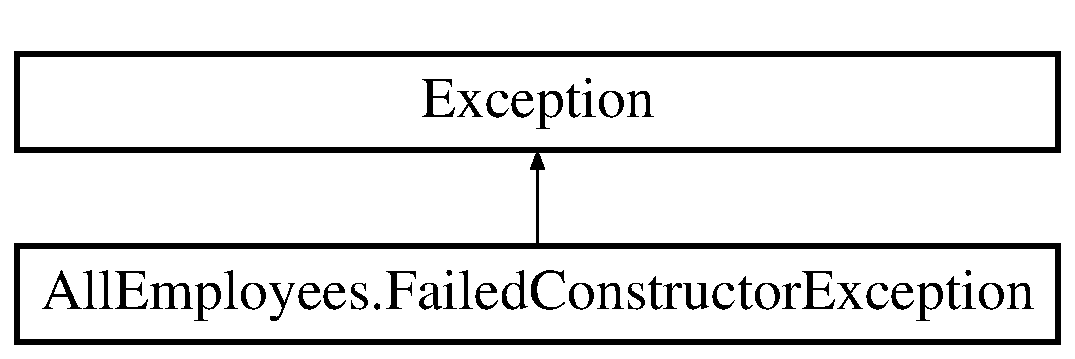
\includegraphics[height=2.000000cm]{class_all_employees_1_1_failed_constructor_exception}
\end{center}
\end{figure}
\subsection*{Public Member Functions}
\begin{DoxyCompactItemize}
\item 
\hyperlink{class_all_employees_1_1_failed_constructor_exception_a78d117eff5ea056d0076b601274f382d}{Failed\+Constructor\+Exception} ()
\begin{DoxyCompactList}\small\item\em default constructor. Create a \hyperlink{class_all_employees_1_1_failed_constructor_exception}{Failed\+Constructor\+Exception} with base Exception class \end{DoxyCompactList}\item 
\hyperlink{class_all_employees_1_1_failed_constructor_exception_a41c940dd9d247e852c71b49788754e9f}{Failed\+Constructor\+Exception} (string message)
\begin{DoxyCompactList}\small\item\em overloaded constructor. Create a \hyperlink{class_all_employees_1_1_failed_constructor_exception}{Failed\+Constructor\+Exception} with base Exception class and message \end{DoxyCompactList}\end{DoxyCompactItemize}


\subsection{Detailed Description}
{\bfseries Brief Description} The \hyperlink{class_all_employees_1_1_failed_constructor_exception}{Failed\+Constructor\+Exception} is a exception that will be thrown if the object the constructor creates is not a valid employee \hyperlink{class_all_employees_1_1_failed_constructor_exception}{Failed\+Constructor\+Exception} is a child of the Exception class 

\begin{DoxyAuthor}{Author}
{\itshape Brandon} 
\end{DoxyAuthor}


\subsection{Constructor \& Destructor Documentation}
\hypertarget{class_all_employees_1_1_failed_constructor_exception_a78d117eff5ea056d0076b601274f382d}{}\index{All\+Employees\+::\+Failed\+Constructor\+Exception@{All\+Employees\+::\+Failed\+Constructor\+Exception}!Failed\+Constructor\+Exception@{Failed\+Constructor\+Exception}}
\index{Failed\+Constructor\+Exception@{Failed\+Constructor\+Exception}!All\+Employees\+::\+Failed\+Constructor\+Exception@{All\+Employees\+::\+Failed\+Constructor\+Exception}}
\subsubsection[{Failed\+Constructor\+Exception}]{\setlength{\rightskip}{0pt plus 5cm}All\+Employees.\+Failed\+Constructor\+Exception.\+Failed\+Constructor\+Exception (
\begin{DoxyParamCaption}
{}
\end{DoxyParamCaption}
)}\label{class_all_employees_1_1_failed_constructor_exception_a78d117eff5ea056d0076b601274f382d}


default constructor. Create a \hyperlink{class_all_employees_1_1_failed_constructor_exception}{Failed\+Constructor\+Exception} with base Exception class 

{\bfseries Details}


\begin{DoxyParams}{Parameters}
{\em n/a} & \\
\hline
\end{DoxyParams}
\begin{DoxyReturn}{Returns}
n/a 
\end{DoxyReturn}
\hypertarget{class_all_employees_1_1_failed_constructor_exception_a41c940dd9d247e852c71b49788754e9f}{}\index{All\+Employees\+::\+Failed\+Constructor\+Exception@{All\+Employees\+::\+Failed\+Constructor\+Exception}!Failed\+Constructor\+Exception@{Failed\+Constructor\+Exception}}
\index{Failed\+Constructor\+Exception@{Failed\+Constructor\+Exception}!All\+Employees\+::\+Failed\+Constructor\+Exception@{All\+Employees\+::\+Failed\+Constructor\+Exception}}
\subsubsection[{Failed\+Constructor\+Exception}]{\setlength{\rightskip}{0pt plus 5cm}All\+Employees.\+Failed\+Constructor\+Exception.\+Failed\+Constructor\+Exception (
\begin{DoxyParamCaption}
\item[{string}]{message}
\end{DoxyParamCaption}
)}\label{class_all_employees_1_1_failed_constructor_exception_a41c940dd9d247e852c71b49788754e9f}


overloaded constructor. Create a \hyperlink{class_all_employees_1_1_failed_constructor_exception}{Failed\+Constructor\+Exception} with base Exception class and message 

{\bfseries Details}


\begin{DoxyParams}{Parameters}
{\em message} & {\bfseries string} -\/ the message to be attached to the exception\\
\hline
\end{DoxyParams}
\begin{DoxyReturn}{Returns}
n/a 
\end{DoxyReturn}


The documentation for this class was generated from the following file\+:\begin{DoxyCompactItemize}
\item 
C\+:/\+S\+E\+T\+Repo/trunk/\+E\+M\+S/trunk/\+All\+Employees/\+All\+Employees/Failed\+Constructor\+Exception.\+cs\end{DoxyCompactItemize}

\hypertarget{class_supporting_1_1_file_i_o}{}\section{Supporting.\+File\+I\+O Class Reference}
\label{class_supporting_1_1_file_i_o}\index{Supporting.\+File\+I\+O@{Supporting.\+File\+I\+O}}


{\bfseries Brief Description} This class allows files to be written to, read all the data from a file, open a file for reading, open a file for writing, closing a file and parsing data from a file. The file\+I\+O class is realted to employee and container class  


\subsection*{Public Member Functions}
\begin{DoxyCompactItemize}
\item 
List$<$ \hyperlink{class_all_employees_1_1_employee}{All\+Employees.\+Employee} $>$ \hyperlink{class_supporting_1_1_file_i_o_ab33154b7acbb27ecaee49cfe701691e7}{Read\+All\+Records} (String file\+Name)
\begin{DoxyCompactList}\small\item\em Give file name, return list of all valid records. \end{DoxyCompactList}\item 
void \hyperlink{class_supporting_1_1_file_i_o_a23293f70ec655e87ea568ffada174b9f}{Write\+Record} (\hyperlink{class_all_employees_1_1_employee}{All\+Employees.\+Employee} Employee, String file\+Name)
\begin{DoxyCompactList}\small\item\em Give employee write and file to write to. \end{DoxyCompactList}\end{DoxyCompactItemize}
\subsection*{Private Member Functions}
\begin{DoxyCompactItemize}
\item 
File\+Stream \hyperlink{class_supporting_1_1_file_i_o_ac9cebd77d6aca1292566d7e6eb4f8123}{Open\+File\+For\+Read} (String file\+Name)
\begin{DoxyCompactList}\small\item\em Give file name, return file for reading. \end{DoxyCompactList}\item 
File\+Stream \hyperlink{class_supporting_1_1_file_i_o_ab3be0f867327310b9d940d79e1147b69}{Open\+File\+For\+Write} (String file\+Name)
\begin{DoxyCompactList}\small\item\em Give file name, return file for writing. \end{DoxyCompactList}\item 
void \hyperlink{class_supporting_1_1_file_i_o_a689379fbd7441f18477d01dfde06444c}{Close\+File} (File\+Stream file)
\begin{DoxyCompactList}\small\item\em Closes the file. \end{DoxyCompactList}\item 
List$<$ \hyperlink{class_all_employees_1_1_employee}{All\+Employees.\+Employee} $>$ \hyperlink{class_supporting_1_1_file_i_o_ab4433298adf44f58cbd355eb5db0bf7f}{Pars\+Record} (String file\+Text)
\begin{DoxyCompactList}\small\item\em given string from file, pars all data into list, return list valid employees \end{DoxyCompactList}\end{DoxyCompactItemize}


\subsection{Detailed Description}
{\bfseries Brief Description} This class allows files to be written to, read all the data from a file, open a file for reading, open a file for writing, closing a file and parsing data from a file. The file\+I\+O class is realted to employee and container class 

\begin{DoxyAuthor}{Author}
{\itshape Nathan} 
\end{DoxyAuthor}


\subsection{Member Function Documentation}
\hypertarget{class_supporting_1_1_file_i_o_a689379fbd7441f18477d01dfde06444c}{}\index{Supporting\+::\+File\+I\+O@{Supporting\+::\+File\+I\+O}!Close\+File@{Close\+File}}
\index{Close\+File@{Close\+File}!Supporting\+::\+File\+I\+O@{Supporting\+::\+File\+I\+O}}
\subsubsection[{Close\+File}]{\setlength{\rightskip}{0pt plus 5cm}void Supporting.\+File\+I\+O.\+Close\+File (
\begin{DoxyParamCaption}
\item[{File\+Stream}]{file}
\end{DoxyParamCaption}
)\hspace{0.3cm}{\ttfamily [private]}}\label{class_supporting_1_1_file_i_o_a689379fbd7441f18477d01dfde06444c}


Closes the file. 

{\bfseries Details}


\begin{DoxyParams}{Parameters}
{\em file} & -\/ {\bfseries File\+Stream} -\/ The file to be closed\\
\hline
\end{DoxyParams}
\begin{DoxyReturn}{Returns}
n/a 
\end{DoxyReturn}
\hypertarget{class_supporting_1_1_file_i_o_ac9cebd77d6aca1292566d7e6eb4f8123}{}\index{Supporting\+::\+File\+I\+O@{Supporting\+::\+File\+I\+O}!Open\+File\+For\+Read@{Open\+File\+For\+Read}}
\index{Open\+File\+For\+Read@{Open\+File\+For\+Read}!Supporting\+::\+File\+I\+O@{Supporting\+::\+File\+I\+O}}
\subsubsection[{Open\+File\+For\+Read}]{\setlength{\rightskip}{0pt plus 5cm}File\+Stream Supporting.\+File\+I\+O.\+Open\+File\+For\+Read (
\begin{DoxyParamCaption}
\item[{String}]{file\+Name}
\end{DoxyParamCaption}
)\hspace{0.3cm}{\ttfamily [private]}}\label{class_supporting_1_1_file_i_o_ac9cebd77d6aca1292566d7e6eb4f8123}


Give file name, return file for reading. 

{\bfseries Details}


\begin{DoxyParams}{Parameters}
{\em file\+Name} & -\/ {\bfseries string} -\/ The file path and name of file storing the records\\
\hline
\end{DoxyParams}
\begin{DoxyReturn}{Returns}
read\+File -\/ {\bfseries File\+Stream} -\/ The opened file to be read 
\end{DoxyReturn}
\hypertarget{class_supporting_1_1_file_i_o_ab3be0f867327310b9d940d79e1147b69}{}\index{Supporting\+::\+File\+I\+O@{Supporting\+::\+File\+I\+O}!Open\+File\+For\+Write@{Open\+File\+For\+Write}}
\index{Open\+File\+For\+Write@{Open\+File\+For\+Write}!Supporting\+::\+File\+I\+O@{Supporting\+::\+File\+I\+O}}
\subsubsection[{Open\+File\+For\+Write}]{\setlength{\rightskip}{0pt plus 5cm}File\+Stream Supporting.\+File\+I\+O.\+Open\+File\+For\+Write (
\begin{DoxyParamCaption}
\item[{String}]{file\+Name}
\end{DoxyParamCaption}
)\hspace{0.3cm}{\ttfamily [private]}}\label{class_supporting_1_1_file_i_o_ab3be0f867327310b9d940d79e1147b69}


Give file name, return file for writing. 

{\bfseries Details}


\begin{DoxyParams}{Parameters}
{\em file\+Name} & -\/ {\bfseries string} -\/ The file path and name of file storing the records\\
\hline
\end{DoxyParams}
\begin{DoxyReturn}{Returns}
write\+File -\/ {\bfseries File\+Stream} -\/ The opened file to be written to 
\end{DoxyReturn}
\hypertarget{class_supporting_1_1_file_i_o_ab4433298adf44f58cbd355eb5db0bf7f}{}\index{Supporting\+::\+File\+I\+O@{Supporting\+::\+File\+I\+O}!Pars\+Record@{Pars\+Record}}
\index{Pars\+Record@{Pars\+Record}!Supporting\+::\+File\+I\+O@{Supporting\+::\+File\+I\+O}}
\subsubsection[{Pars\+Record}]{\setlength{\rightskip}{0pt plus 5cm}List$<${\bf All\+Employees.\+Employee}$>$ Supporting.\+File\+I\+O.\+Pars\+Record (
\begin{DoxyParamCaption}
\item[{String}]{file\+Text}
\end{DoxyParamCaption}
)\hspace{0.3cm}{\ttfamily [private]}}\label{class_supporting_1_1_file_i_o_ab4433298adf44f58cbd355eb5db0bf7f}


given string from file, pars all data into list, return list valid employees 

{\bfseries Details}


\begin{DoxyParams}{Parameters}
{\em file\+Text} & -\/ {\bfseries string} -\/ The string of data containing an employees records\\
\hline
\end{DoxyParams}
\begin{DoxyReturn}{Returns}
employee\+Rec -\/ {\bfseries List$<$\+All\+Employees.\+Employee$>$} -\/ The list of all the employee records in the strinng of data 
\end{DoxyReturn}
\hypertarget{class_supporting_1_1_file_i_o_ab33154b7acbb27ecaee49cfe701691e7}{}\index{Supporting\+::\+File\+I\+O@{Supporting\+::\+File\+I\+O}!Read\+All\+Records@{Read\+All\+Records}}
\index{Read\+All\+Records@{Read\+All\+Records}!Supporting\+::\+File\+I\+O@{Supporting\+::\+File\+I\+O}}
\subsubsection[{Read\+All\+Records}]{\setlength{\rightskip}{0pt plus 5cm}List$<${\bf All\+Employees.\+Employee}$>$ Supporting.\+File\+I\+O.\+Read\+All\+Records (
\begin{DoxyParamCaption}
\item[{String}]{file\+Name}
\end{DoxyParamCaption}
)}\label{class_supporting_1_1_file_i_o_ab33154b7acbb27ecaee49cfe701691e7}


Give file name, return list of all valid records. 

{\bfseries Details}


\begin{DoxyParams}{Parameters}
{\em file\+Name} & -\/ {\bfseries string} -\/ The file path and name of file storing the records\\
\hline
\end{DoxyParams}
\begin{DoxyReturn}{Returns}
employee\+Rec -\/ {\bfseries List$<$\+All\+Employees.\+Employee$>$} -\/ The list of all the employee records in the file 
\end{DoxyReturn}
\hypertarget{class_supporting_1_1_file_i_o_a23293f70ec655e87ea568ffada174b9f}{}\index{Supporting\+::\+File\+I\+O@{Supporting\+::\+File\+I\+O}!Write\+Record@{Write\+Record}}
\index{Write\+Record@{Write\+Record}!Supporting\+::\+File\+I\+O@{Supporting\+::\+File\+I\+O}}
\subsubsection[{Write\+Record}]{\setlength{\rightskip}{0pt plus 5cm}void Supporting.\+File\+I\+O.\+Write\+Record (
\begin{DoxyParamCaption}
\item[{{\bf All\+Employees.\+Employee}}]{Employee, }
\item[{String}]{file\+Name}
\end{DoxyParamCaption}
)}\label{class_supporting_1_1_file_i_o_a23293f70ec655e87ea568ffada174b9f}


Give employee write and file to write to. 

{\bfseries Details}


\begin{DoxyParams}{Parameters}
{\em Employee} & -\/ {\bfseries \hyperlink{class_all_employees_1_1_employee}{All\+Employees.\+Employee}} -\/ The employees records \\
\hline
{\em file\+Name} & -\/ {\bfseries String} -\/ The file path and name of file storing the records\\
\hline
\end{DoxyParams}
\begin{DoxyReturn}{Returns}
n/a 
\end{DoxyReturn}


The documentation for this class was generated from the following file\+:\begin{DoxyCompactItemize}
\item 
C\+:/\+S\+E\+T\+Repo/trunk/\+E\+M\+S/trunk/\+Supporting/\+Supporting/File\+I\+O.\+cs\end{DoxyCompactItemize}

\hypertarget{class_all_employees_1_1_fulltime_employee}{}\section{All\+Employees.\+Fulltime\+Employee Class Reference}
\label{class_all_employees_1_1_fulltime_employee}\index{All\+Employees.\+Fulltime\+Employee@{All\+Employees.\+Fulltime\+Employee}}


{\bfseries Brief Description} The Fulltime \hyperlink{class_all_employees_1_1_employee}{Employee} class is used to store and manage data about a employee who is hired for a full-\/time position. This class is a child to \hyperlink{class_all_employees_1_1_employee}{Employee} class. It adds the date of hire and termination, and the employees salary. If the constructor creates a invalid employee, a exception is thrown. All other errors result in a defined return.  


Inheritance diagram for All\+Employees.\+Fulltime\+Employee\+:\begin{figure}[H]
\begin{center}
\leavevmode
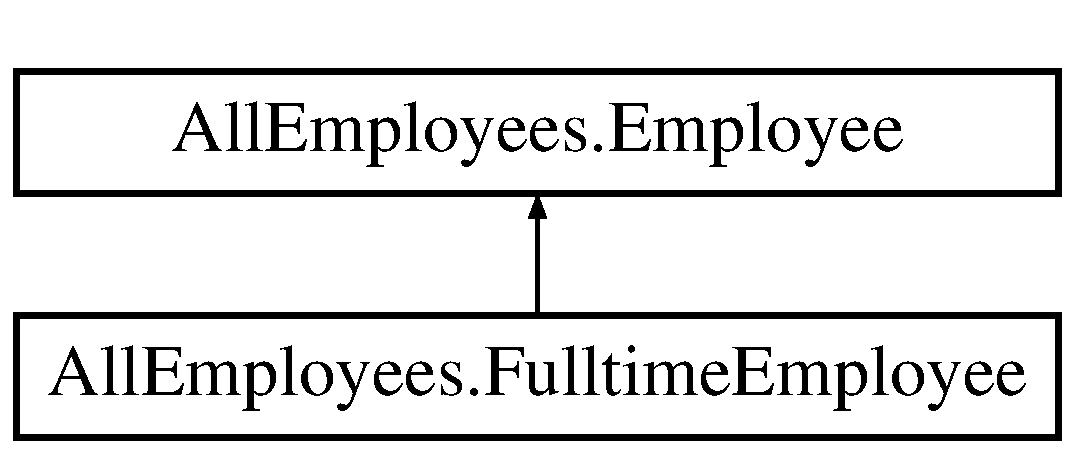
\includegraphics[height=2.000000cm]{class_all_employees_1_1_fulltime_employee}
\end{center}
\end{figure}
\subsection*{Public Member Functions}
\begin{DoxyCompactItemize}
\item 
\hyperlink{class_all_employees_1_1_fulltime_employee_a2f7744fed20aa3161c5ac5cd37c1a281}{Fulltime\+Employee} ()
\begin{DoxyCompactList}\small\item\em default constructor. Sets all values to default \end{DoxyCompactList}\item 
\hyperlink{class_all_employees_1_1_fulltime_employee_a7cc8db6b3e7dd2fa71706c9ebaf68660}{Fulltime\+Employee} (string first\+Name, string last\+Name)
\begin{DoxyCompactList}\small\item\em overloaded constructor. Sets name to inputed names, set all other values to default \end{DoxyCompactList}\item 
\hyperlink{class_all_employees_1_1_fulltime_employee_abf4afc245af7d4d99452ef6251415317}{Fulltime\+Employee} (string first\+Name, string last\+Name, int social\+Insurance\+Number, Date\+Time date\+Of\+Birth, Date\+Time date\+Of\+Hire, Date\+Time date\+Of\+Termination, float salary)
\begin{DoxyCompactList}\small\item\em overloaded constructor. Sets all values to the values given. no default values \end{DoxyCompactList}\item 
bool \hyperlink{class_all_employees_1_1_fulltime_employee_a3e718749e4730c0f2a28f820530071da}{Validate} ()
\begin{DoxyCompactList}\small\item\em Used to determine in the object contains a valid employee. \end{DoxyCompactList}\item 
string \hyperlink{class_all_employees_1_1_fulltime_employee_a7660032e944e78c6ff26598aa7107796}{Details} ()
\begin{DoxyCompactList}\small\item\em Used to print all employee data to the consol. \end{DoxyCompactList}\item 
override string \hyperlink{class_all_employees_1_1_fulltime_employee_a3026e5a4c764fc0da54873cc131e2b82}{To\+String} ()
\begin{DoxyCompactList}\small\item\em Overriden method To\+String used to return a formated string of all data. \end{DoxyCompactList}\item 
bool \hyperlink{class_all_employees_1_1_fulltime_employee_aaf2dc1dcb158819d06958d4399850f56}{Set\+Date\+Of\+Hire} (Date\+Time date)
\begin{DoxyCompactList}\small\item\em Setter for date\+Of\+Hire. \end{DoxyCompactList}\item 
bool \hyperlink{class_all_employees_1_1_fulltime_employee_a6b7516d71f46e650da2200a308d6f226}{Set\+Date\+Of\+Hire} (string date)
\begin{DoxyCompactList}\small\item\em Setter for date\+Of\+Hire from String. \end{DoxyCompactList}\item 
bool \hyperlink{class_all_employees_1_1_fulltime_employee_ae5612c076ead69a3b6f0bbc22a21e293}{Set\+Date\+Of\+Hire} (int year, int month, int day)
\begin{DoxyCompactList}\small\item\em Setter for date\+Of\+Hire from ints. \end{DoxyCompactList}\item 
bool \hyperlink{class_all_employees_1_1_fulltime_employee_a94e9d4b67b20ecbe1449701a200b1c07}{Set\+Date\+Of\+Termination} (Date\+Time date)
\begin{DoxyCompactList}\small\item\em Setter for date\+Of\+Termination. \end{DoxyCompactList}\item 
bool \hyperlink{class_all_employees_1_1_fulltime_employee_a7d142370fe7f81bd623de155a80d0214}{Set\+Date\+Of\+Termination} (string date)
\begin{DoxyCompactList}\small\item\em Setter for date\+Of\+Termination from string. \end{DoxyCompactList}\item 
bool \hyperlink{class_all_employees_1_1_fulltime_employee_aed4ff527256f96b542d0ac0c17f3e2ea}{Set\+Date\+Of\+Termination} (int year, int month, int day)
\begin{DoxyCompactList}\small\item\em Setter for date\+Of\+Termination from int. \end{DoxyCompactList}\item 
bool \hyperlink{class_all_employees_1_1_fulltime_employee_accdd74311a5e97d8beb57d68bd88f95c}{Set\+Salary} (float salary)
\begin{DoxyCompactList}\small\item\em Setter for salary. \end{DoxyCompactList}\item 
Date\+Time \hyperlink{class_all_employees_1_1_fulltime_employee_a3a975ad60176797d1d5529e257596565}{Get\+Date\+Of\+Hire} ()
\begin{DoxyCompactList}\small\item\em Getter for date\+Of\+Hire. \end{DoxyCompactList}\item 
string \hyperlink{class_all_employees_1_1_fulltime_employee_a91b4f15454d92eb7cd33968573050ef0}{Get\+Date\+Of\+Hire\+String} ()
\begin{DoxyCompactList}\small\item\em Getter for date\+Of\+Hire that returns formatted string. \end{DoxyCompactList}\item 
Date\+Time \hyperlink{class_all_employees_1_1_fulltime_employee_a97af3da9151f97e91543d60b6b67a4fa}{Get\+Date\+Of\+Termination} ()
\begin{DoxyCompactList}\small\item\em Getter for date\+Of\+Termination. \end{DoxyCompactList}\item 
string \hyperlink{class_all_employees_1_1_fulltime_employee_a7d0612eba21e83226bb09a174179847c}{Get\+Date\+Of\+Termination\+String} ()
\begin{DoxyCompactList}\small\item\em Getter for date\+Of\+Termination that returns formatted string. \end{DoxyCompactList}\item 
float \hyperlink{class_all_employees_1_1_fulltime_employee_a919105156f70d21baa1f3ce5f4d160ee}{Get\+Salary} ()
\begin{DoxyCompactList}\small\item\em Getter for salary. \end{DoxyCompactList}\end{DoxyCompactItemize}
\subsection*{Private Attributes}
\begin{DoxyCompactItemize}
\item 
\hypertarget{class_all_employees_1_1_fulltime_employee_aa072bd7c652567684c77e0cfd6638af2}{}Date\+Time {\bfseries date\+Of\+Hire}\label{class_all_employees_1_1_fulltime_employee_aa072bd7c652567684c77e0cfd6638af2}

\item 
\hypertarget{class_all_employees_1_1_fulltime_employee_a3836c1a3f74f71f87652c91913eb570c}{}Date\+Time {\bfseries date\+Of\+Termination}\label{class_all_employees_1_1_fulltime_employee_a3836c1a3f74f71f87652c91913eb570c}

\item 
\hypertarget{class_all_employees_1_1_fulltime_employee_afd766110662d0321998cecb84d0dd425}{}float {\bfseries salary}\label{class_all_employees_1_1_fulltime_employee_afd766110662d0321998cecb84d0dd425}

\end{DoxyCompactItemize}
\subsection*{Additional Inherited Members}


\subsection{Detailed Description}
{\bfseries Brief Description} The Fulltime \hyperlink{class_all_employees_1_1_employee}{Employee} class is used to store and manage data about a employee who is hired for a full-\/time position. This class is a child to \hyperlink{class_all_employees_1_1_employee}{Employee} class. It adds the date of hire and termination, and the employees salary. If the constructor creates a invalid employee, a exception is thrown. All other errors result in a defined return. 

\begin{DoxyAuthor}{Author}
{\itshape Brandon} 
\end{DoxyAuthor}


\subsection{Constructor \& Destructor Documentation}
\hypertarget{class_all_employees_1_1_fulltime_employee_a2f7744fed20aa3161c5ac5cd37c1a281}{}\index{All\+Employees\+::\+Fulltime\+Employee@{All\+Employees\+::\+Fulltime\+Employee}!Fulltime\+Employee@{Fulltime\+Employee}}
\index{Fulltime\+Employee@{Fulltime\+Employee}!All\+Employees\+::\+Fulltime\+Employee@{All\+Employees\+::\+Fulltime\+Employee}}
\subsubsection[{Fulltime\+Employee}]{\setlength{\rightskip}{0pt plus 5cm}All\+Employees.\+Fulltime\+Employee.\+Fulltime\+Employee (
\begin{DoxyParamCaption}
{}
\end{DoxyParamCaption}
)}\label{class_all_employees_1_1_fulltime_employee_a2f7744fed20aa3161c5ac5cd37c1a281}


default constructor. Sets all values to default 

{\bfseries Details}


\begin{DoxyParams}{Parameters}
{\em n/a} & \\
\hline
\end{DoxyParams}
\begin{DoxyReturn}{Returns}
n/a 
\end{DoxyReturn}
\hypertarget{class_all_employees_1_1_fulltime_employee_a7cc8db6b3e7dd2fa71706c9ebaf68660}{}\index{All\+Employees\+::\+Fulltime\+Employee@{All\+Employees\+::\+Fulltime\+Employee}!Fulltime\+Employee@{Fulltime\+Employee}}
\index{Fulltime\+Employee@{Fulltime\+Employee}!All\+Employees\+::\+Fulltime\+Employee@{All\+Employees\+::\+Fulltime\+Employee}}
\subsubsection[{Fulltime\+Employee}]{\setlength{\rightskip}{0pt plus 5cm}All\+Employees.\+Fulltime\+Employee.\+Fulltime\+Employee (
\begin{DoxyParamCaption}
\item[{string}]{first\+Name, }
\item[{string}]{last\+Name}
\end{DoxyParamCaption}
)}\label{class_all_employees_1_1_fulltime_employee_a7cc8db6b3e7dd2fa71706c9ebaf68660}


overloaded constructor. Sets name to inputed names, set all other values to default 

{\bfseries Details}


\begin{DoxyParams}{Parameters}
{\em first\+Name} & -\/ {\bfseries string} -\/ First Name of employee to add to records \\
\hline
{\em last\+Name} & -\/ {\bfseries string} -\/ Last Name of employee to add to records\\
\hline
\end{DoxyParams}

\begin{DoxyExceptions}{Exceptions}
{\em $<$\+Failed\+Constructor\+Exception$>$} & -\/ If the constructor failed to create the object\\
\hline
\end{DoxyExceptions}
\begin{DoxyReturn}{Returns}
n/a 
\end{DoxyReturn}
\hypertarget{class_all_employees_1_1_fulltime_employee_abf4afc245af7d4d99452ef6251415317}{}\index{All\+Employees\+::\+Fulltime\+Employee@{All\+Employees\+::\+Fulltime\+Employee}!Fulltime\+Employee@{Fulltime\+Employee}}
\index{Fulltime\+Employee@{Fulltime\+Employee}!All\+Employees\+::\+Fulltime\+Employee@{All\+Employees\+::\+Fulltime\+Employee}}
\subsubsection[{Fulltime\+Employee}]{\setlength{\rightskip}{0pt plus 5cm}All\+Employees.\+Fulltime\+Employee.\+Fulltime\+Employee (
\begin{DoxyParamCaption}
\item[{string}]{first\+Name, }
\item[{string}]{last\+Name, }
\item[{int}]{social\+Insurance\+Number, }
\item[{Date\+Time}]{date\+Of\+Birth, }
\item[{Date\+Time}]{date\+Of\+Hire, }
\item[{Date\+Time}]{date\+Of\+Termination, }
\item[{float}]{salary}
\end{DoxyParamCaption}
)}\label{class_all_employees_1_1_fulltime_employee_abf4afc245af7d4d99452ef6251415317}


overloaded constructor. Sets all values to the values given. no default values 

{\bfseries Details}


\begin{DoxyParams}{Parameters}
{\em first\+Name} & -\/ {\bfseries string} -\/ First Name of employee to add to records \\
\hline
{\em last\+Name} & -\/ {\bfseries string} -\/ Last Name of employee to add to records \\
\hline
{\em social\+Insurance\+Number} & -\/ {\bfseries int} -\/ Social Insurance Number of employee to add to records \\
\hline
{\em date\+Of\+Birth} & -\/ {\bfseries Date\+Time} -\/ Date Of Birth of employee to add to records \\
\hline
{\em date\+Of\+Hire} & -\/ {\bfseries Date\+Time} -\/ Date Of Hire of employee to add to records \\
\hline
{\em date\+Of\+Termination} & -\/ {\bfseries Date\+Time} -\/ Date Of Termination of employee to add to records \\
\hline
{\em salary} & -\/ {\bfseries float} -\/ salary of employee to add to records\\
\hline
\end{DoxyParams}

\begin{DoxyExceptions}{Exceptions}
{\em $<$\+Failed\+Constructor\+Exception$>$} & -\/ If the constructor failed to create the object\\
\hline
\end{DoxyExceptions}
\begin{DoxyReturn}{Returns}
n/a 
\end{DoxyReturn}


\subsection{Member Function Documentation}
\hypertarget{class_all_employees_1_1_fulltime_employee_a7660032e944e78c6ff26598aa7107796}{}\index{All\+Employees\+::\+Fulltime\+Employee@{All\+Employees\+::\+Fulltime\+Employee}!Details@{Details}}
\index{Details@{Details}!All\+Employees\+::\+Fulltime\+Employee@{All\+Employees\+::\+Fulltime\+Employee}}
\subsubsection[{Details}]{\setlength{\rightskip}{0pt plus 5cm}string All\+Employees.\+Fulltime\+Employee.\+Details (
\begin{DoxyParamCaption}
{}
\end{DoxyParamCaption}
)}\label{class_all_employees_1_1_fulltime_employee_a7660032e944e78c6ff26598aa7107796}


Used to print all employee data to the consol. 

{\bfseries Details}


\begin{DoxyParams}{Parameters}
{\em n/a} & \\
\hline
\end{DoxyParams}
\begin{DoxyReturn}{Returns}
user\+Info {\bfseries string} -\/ formatted string of employee data 
\end{DoxyReturn}
\hypertarget{class_all_employees_1_1_fulltime_employee_a3a975ad60176797d1d5529e257596565}{}\index{All\+Employees\+::\+Fulltime\+Employee@{All\+Employees\+::\+Fulltime\+Employee}!Get\+Date\+Of\+Hire@{Get\+Date\+Of\+Hire}}
\index{Get\+Date\+Of\+Hire@{Get\+Date\+Of\+Hire}!All\+Employees\+::\+Fulltime\+Employee@{All\+Employees\+::\+Fulltime\+Employee}}
\subsubsection[{Get\+Date\+Of\+Hire}]{\setlength{\rightskip}{0pt plus 5cm}Date\+Time All\+Employees.\+Fulltime\+Employee.\+Get\+Date\+Of\+Hire (
\begin{DoxyParamCaption}
{}
\end{DoxyParamCaption}
)}\label{class_all_employees_1_1_fulltime_employee_a3a975ad60176797d1d5529e257596565}


Getter for date\+Of\+Hire. 

{\bfseries Details}


\begin{DoxyParams}{Parameters}
{\em n/a} & \\
\hline
\end{DoxyParams}
\begin{DoxyReturn}{Returns}
date\+Of\+Hire {\bfseries Date\+Time} 
\end{DoxyReturn}
\hypertarget{class_all_employees_1_1_fulltime_employee_a91b4f15454d92eb7cd33968573050ef0}{}\index{All\+Employees\+::\+Fulltime\+Employee@{All\+Employees\+::\+Fulltime\+Employee}!Get\+Date\+Of\+Hire\+String@{Get\+Date\+Of\+Hire\+String}}
\index{Get\+Date\+Of\+Hire\+String@{Get\+Date\+Of\+Hire\+String}!All\+Employees\+::\+Fulltime\+Employee@{All\+Employees\+::\+Fulltime\+Employee}}
\subsubsection[{Get\+Date\+Of\+Hire\+String}]{\setlength{\rightskip}{0pt plus 5cm}string All\+Employees.\+Fulltime\+Employee.\+Get\+Date\+Of\+Hire\+String (
\begin{DoxyParamCaption}
{}
\end{DoxyParamCaption}
)}\label{class_all_employees_1_1_fulltime_employee_a91b4f15454d92eb7cd33968573050ef0}


Getter for date\+Of\+Hire that returns formatted string. 

{\bfseries Details}


\begin{DoxyParams}{Parameters}
{\em n/a} & \\
\hline
\end{DoxyParams}
\begin{DoxyReturn}{Returns}
date\+Of\+Hire {\bfseries string} 
\end{DoxyReturn}
\hypertarget{class_all_employees_1_1_fulltime_employee_a97af3da9151f97e91543d60b6b67a4fa}{}\index{All\+Employees\+::\+Fulltime\+Employee@{All\+Employees\+::\+Fulltime\+Employee}!Get\+Date\+Of\+Termination@{Get\+Date\+Of\+Termination}}
\index{Get\+Date\+Of\+Termination@{Get\+Date\+Of\+Termination}!All\+Employees\+::\+Fulltime\+Employee@{All\+Employees\+::\+Fulltime\+Employee}}
\subsubsection[{Get\+Date\+Of\+Termination}]{\setlength{\rightskip}{0pt plus 5cm}Date\+Time All\+Employees.\+Fulltime\+Employee.\+Get\+Date\+Of\+Termination (
\begin{DoxyParamCaption}
{}
\end{DoxyParamCaption}
)}\label{class_all_employees_1_1_fulltime_employee_a97af3da9151f97e91543d60b6b67a4fa}


Getter for date\+Of\+Termination. 

{\bfseries Details}


\begin{DoxyParams}{Parameters}
{\em n/a} & \\
\hline
\end{DoxyParams}
\begin{DoxyReturn}{Returns}
date\+Of\+Termination {\bfseries Date\+Time} 
\end{DoxyReturn}
\hypertarget{class_all_employees_1_1_fulltime_employee_a7d0612eba21e83226bb09a174179847c}{}\index{All\+Employees\+::\+Fulltime\+Employee@{All\+Employees\+::\+Fulltime\+Employee}!Get\+Date\+Of\+Termination\+String@{Get\+Date\+Of\+Termination\+String}}
\index{Get\+Date\+Of\+Termination\+String@{Get\+Date\+Of\+Termination\+String}!All\+Employees\+::\+Fulltime\+Employee@{All\+Employees\+::\+Fulltime\+Employee}}
\subsubsection[{Get\+Date\+Of\+Termination\+String}]{\setlength{\rightskip}{0pt plus 5cm}string All\+Employees.\+Fulltime\+Employee.\+Get\+Date\+Of\+Termination\+String (
\begin{DoxyParamCaption}
{}
\end{DoxyParamCaption}
)}\label{class_all_employees_1_1_fulltime_employee_a7d0612eba21e83226bb09a174179847c}


Getter for date\+Of\+Termination that returns formatted string. 

{\bfseries Details}


\begin{DoxyParams}{Parameters}
{\em n/a} & \\
\hline
\end{DoxyParams}
\begin{DoxyReturn}{Returns}
date\+Of\+Termination {\bfseries string} 
\end{DoxyReturn}
\hypertarget{class_all_employees_1_1_fulltime_employee_a919105156f70d21baa1f3ce5f4d160ee}{}\index{All\+Employees\+::\+Fulltime\+Employee@{All\+Employees\+::\+Fulltime\+Employee}!Get\+Salary@{Get\+Salary}}
\index{Get\+Salary@{Get\+Salary}!All\+Employees\+::\+Fulltime\+Employee@{All\+Employees\+::\+Fulltime\+Employee}}
\subsubsection[{Get\+Salary}]{\setlength{\rightskip}{0pt plus 5cm}float All\+Employees.\+Fulltime\+Employee.\+Get\+Salary (
\begin{DoxyParamCaption}
{}
\end{DoxyParamCaption}
)}\label{class_all_employees_1_1_fulltime_employee_a919105156f70d21baa1f3ce5f4d160ee}


Getter for salary. 

{\bfseries Details}


\begin{DoxyParams}{Parameters}
{\em n/a} & \\
\hline
\end{DoxyParams}
\begin{DoxyReturn}{Returns}
salary {\bfseries float} 
\end{DoxyReturn}
\hypertarget{class_all_employees_1_1_fulltime_employee_aaf2dc1dcb158819d06958d4399850f56}{}\index{All\+Employees\+::\+Fulltime\+Employee@{All\+Employees\+::\+Fulltime\+Employee}!Set\+Date\+Of\+Hire@{Set\+Date\+Of\+Hire}}
\index{Set\+Date\+Of\+Hire@{Set\+Date\+Of\+Hire}!All\+Employees\+::\+Fulltime\+Employee@{All\+Employees\+::\+Fulltime\+Employee}}
\subsubsection[{Set\+Date\+Of\+Hire}]{\setlength{\rightskip}{0pt plus 5cm}bool All\+Employees.\+Fulltime\+Employee.\+Set\+Date\+Of\+Hire (
\begin{DoxyParamCaption}
\item[{Date\+Time}]{date}
\end{DoxyParamCaption}
)}\label{class_all_employees_1_1_fulltime_employee_aaf2dc1dcb158819d06958d4399850f56}


Setter for date\+Of\+Hire. 

{\bfseries Details}


\begin{DoxyParams}{Parameters}
{\em date} & {\bfseries Date\+Time} -\/ The employees date of hire\\
\hline
\end{DoxyParams}
\begin{DoxyReturn}{Returns}
data\+Saved {\bfseries bool} -\/ true if input was valid and data was changed. False it data was not changed 
\end{DoxyReturn}
\hypertarget{class_all_employees_1_1_fulltime_employee_a6b7516d71f46e650da2200a308d6f226}{}\index{All\+Employees\+::\+Fulltime\+Employee@{All\+Employees\+::\+Fulltime\+Employee}!Set\+Date\+Of\+Hire@{Set\+Date\+Of\+Hire}}
\index{Set\+Date\+Of\+Hire@{Set\+Date\+Of\+Hire}!All\+Employees\+::\+Fulltime\+Employee@{All\+Employees\+::\+Fulltime\+Employee}}
\subsubsection[{Set\+Date\+Of\+Hire}]{\setlength{\rightskip}{0pt plus 5cm}bool All\+Employees.\+Fulltime\+Employee.\+Set\+Date\+Of\+Hire (
\begin{DoxyParamCaption}
\item[{string}]{date}
\end{DoxyParamCaption}
)}\label{class_all_employees_1_1_fulltime_employee_a6b7516d71f46e650da2200a308d6f226}


Setter for date\+Of\+Hire from String. 

{\bfseries Details}


\begin{DoxyParams}{Parameters}
{\em date} & {\bfseries string} -\/ The employees date of hire\\
\hline
\end{DoxyParams}
\begin{DoxyReturn}{Returns}
data\+Saved {\bfseries bool} -\/ true if input was valid and data was changed. False it data was not changed 
\end{DoxyReturn}
\hypertarget{class_all_employees_1_1_fulltime_employee_ae5612c076ead69a3b6f0bbc22a21e293}{}\index{All\+Employees\+::\+Fulltime\+Employee@{All\+Employees\+::\+Fulltime\+Employee}!Set\+Date\+Of\+Hire@{Set\+Date\+Of\+Hire}}
\index{Set\+Date\+Of\+Hire@{Set\+Date\+Of\+Hire}!All\+Employees\+::\+Fulltime\+Employee@{All\+Employees\+::\+Fulltime\+Employee}}
\subsubsection[{Set\+Date\+Of\+Hire}]{\setlength{\rightskip}{0pt plus 5cm}bool All\+Employees.\+Fulltime\+Employee.\+Set\+Date\+Of\+Hire (
\begin{DoxyParamCaption}
\item[{int}]{year, }
\item[{int}]{month, }
\item[{int}]{day}
\end{DoxyParamCaption}
)}\label{class_all_employees_1_1_fulltime_employee_ae5612c076ead69a3b6f0bbc22a21e293}


Setter for date\+Of\+Hire from ints. 

{\bfseries Details}


\begin{DoxyParams}{Parameters}
{\em year} & {\bfseries int} -\/ The start year of the employees date of hire \\
\hline
{\em month} & {\bfseries int} -\/ The start month of the employees date of hire \\
\hline
{\em day} & {\bfseries int} -\/ The start day of the employees date of hire\\
\hline
\end{DoxyParams}
\begin{DoxyReturn}{Returns}
data\+Saved {\bfseries bool} -\/ true if input was valid and data was changed. False it data was not changed 
\end{DoxyReturn}
\hypertarget{class_all_employees_1_1_fulltime_employee_a94e9d4b67b20ecbe1449701a200b1c07}{}\index{All\+Employees\+::\+Fulltime\+Employee@{All\+Employees\+::\+Fulltime\+Employee}!Set\+Date\+Of\+Termination@{Set\+Date\+Of\+Termination}}
\index{Set\+Date\+Of\+Termination@{Set\+Date\+Of\+Termination}!All\+Employees\+::\+Fulltime\+Employee@{All\+Employees\+::\+Fulltime\+Employee}}
\subsubsection[{Set\+Date\+Of\+Termination}]{\setlength{\rightskip}{0pt plus 5cm}bool All\+Employees.\+Fulltime\+Employee.\+Set\+Date\+Of\+Termination (
\begin{DoxyParamCaption}
\item[{Date\+Time}]{date}
\end{DoxyParamCaption}
)}\label{class_all_employees_1_1_fulltime_employee_a94e9d4b67b20ecbe1449701a200b1c07}


Setter for date\+Of\+Termination. 

{\bfseries Details}


\begin{DoxyParams}{Parameters}
{\em date} & {\bfseries Date\+Time} -\/ The employees date of termination\\
\hline
\end{DoxyParams}
\begin{DoxyReturn}{Returns}
data\+Saved {\bfseries bool} -\/ true if input was valid and data was changed. False it data was not changed 
\end{DoxyReturn}
\hypertarget{class_all_employees_1_1_fulltime_employee_a7d142370fe7f81bd623de155a80d0214}{}\index{All\+Employees\+::\+Fulltime\+Employee@{All\+Employees\+::\+Fulltime\+Employee}!Set\+Date\+Of\+Termination@{Set\+Date\+Of\+Termination}}
\index{Set\+Date\+Of\+Termination@{Set\+Date\+Of\+Termination}!All\+Employees\+::\+Fulltime\+Employee@{All\+Employees\+::\+Fulltime\+Employee}}
\subsubsection[{Set\+Date\+Of\+Termination}]{\setlength{\rightskip}{0pt plus 5cm}bool All\+Employees.\+Fulltime\+Employee.\+Set\+Date\+Of\+Termination (
\begin{DoxyParamCaption}
\item[{string}]{date}
\end{DoxyParamCaption}
)}\label{class_all_employees_1_1_fulltime_employee_a7d142370fe7f81bd623de155a80d0214}


Setter for date\+Of\+Termination from string. 

{\bfseries Details}


\begin{DoxyParams}{Parameters}
{\em date} & {\bfseries string} -\/ The employees date of termination\\
\hline
\end{DoxyParams}
\begin{DoxyReturn}{Returns}
data\+Saved {\bfseries bool} -\/ true if input was valid and data was changed. False it data was not changed 
\end{DoxyReturn}
\hypertarget{class_all_employees_1_1_fulltime_employee_aed4ff527256f96b542d0ac0c17f3e2ea}{}\index{All\+Employees\+::\+Fulltime\+Employee@{All\+Employees\+::\+Fulltime\+Employee}!Set\+Date\+Of\+Termination@{Set\+Date\+Of\+Termination}}
\index{Set\+Date\+Of\+Termination@{Set\+Date\+Of\+Termination}!All\+Employees\+::\+Fulltime\+Employee@{All\+Employees\+::\+Fulltime\+Employee}}
\subsubsection[{Set\+Date\+Of\+Termination}]{\setlength{\rightskip}{0pt plus 5cm}bool All\+Employees.\+Fulltime\+Employee.\+Set\+Date\+Of\+Termination (
\begin{DoxyParamCaption}
\item[{int}]{year, }
\item[{int}]{month, }
\item[{int}]{day}
\end{DoxyParamCaption}
)}\label{class_all_employees_1_1_fulltime_employee_aed4ff527256f96b542d0ac0c17f3e2ea}


Setter for date\+Of\+Termination from int. 

{\bfseries Details}


\begin{DoxyParams}{Parameters}
{\em year} & {\bfseries int} -\/ The start year of the employees date of termination \\
\hline
{\em month} & {\bfseries int} -\/ The start month of the employees date of termination \\
\hline
{\em day} & {\bfseries int} -\/ The start day of the employees date of termination\\
\hline
\end{DoxyParams}
\begin{DoxyReturn}{Returns}
data\+Saved {\bfseries bool} -\/ true if input was valid and data was changed. False it data was not changed 
\end{DoxyReturn}
\hypertarget{class_all_employees_1_1_fulltime_employee_accdd74311a5e97d8beb57d68bd88f95c}{}\index{All\+Employees\+::\+Fulltime\+Employee@{All\+Employees\+::\+Fulltime\+Employee}!Set\+Salary@{Set\+Salary}}
\index{Set\+Salary@{Set\+Salary}!All\+Employees\+::\+Fulltime\+Employee@{All\+Employees\+::\+Fulltime\+Employee}}
\subsubsection[{Set\+Salary}]{\setlength{\rightskip}{0pt plus 5cm}bool All\+Employees.\+Fulltime\+Employee.\+Set\+Salary (
\begin{DoxyParamCaption}
\item[{float}]{salary}
\end{DoxyParamCaption}
)}\label{class_all_employees_1_1_fulltime_employee_accdd74311a5e97d8beb57d68bd88f95c}


Setter for salary. 

{\bfseries Details}


\begin{DoxyParams}{Parameters}
{\em salary} & {\bfseries float} -\/ The salary of the employee\\
\hline
\end{DoxyParams}
\begin{DoxyReturn}{Returns}
data\+Saved {\bfseries bool} -\/ true if input was valid and data was changed. False it data was not changed 
\end{DoxyReturn}
\hypertarget{class_all_employees_1_1_fulltime_employee_a3026e5a4c764fc0da54873cc131e2b82}{}\index{All\+Employees\+::\+Fulltime\+Employee@{All\+Employees\+::\+Fulltime\+Employee}!To\+String@{To\+String}}
\index{To\+String@{To\+String}!All\+Employees\+::\+Fulltime\+Employee@{All\+Employees\+::\+Fulltime\+Employee}}
\subsubsection[{To\+String}]{\setlength{\rightskip}{0pt plus 5cm}override string All\+Employees.\+Fulltime\+Employee.\+To\+String (
\begin{DoxyParamCaption}
{}
\end{DoxyParamCaption}
)}\label{class_all_employees_1_1_fulltime_employee_a3026e5a4c764fc0da54873cc131e2b82}


Overriden method To\+String used to return a formated string of all data. 

{\bfseries Details}


\begin{DoxyParams}{Parameters}
{\em n/a} & \\
\hline
\end{DoxyParams}
\begin{DoxyReturn}{Returns}
employee\+String {\bfseries string} -\/ the formated string containing all employee data 
\end{DoxyReturn}
\hypertarget{class_all_employees_1_1_fulltime_employee_a3e718749e4730c0f2a28f820530071da}{}\index{All\+Employees\+::\+Fulltime\+Employee@{All\+Employees\+::\+Fulltime\+Employee}!Validate@{Validate}}
\index{Validate@{Validate}!All\+Employees\+::\+Fulltime\+Employee@{All\+Employees\+::\+Fulltime\+Employee}}
\subsubsection[{Validate}]{\setlength{\rightskip}{0pt plus 5cm}bool All\+Employees.\+Fulltime\+Employee.\+Validate (
\begin{DoxyParamCaption}
{}
\end{DoxyParamCaption}
)}\label{class_all_employees_1_1_fulltime_employee_a3e718749e4730c0f2a28f820530071da}


Used to determine in the object contains a valid employee. 

{\bfseries Details}


\begin{DoxyParams}{Parameters}
{\em n/a} & \\
\hline
\end{DoxyParams}
\begin{DoxyReturn}{Returns}
data\+Valid -\/ {\bfseries bool} -\/ True if the object contains all data for a valid employee 
\end{DoxyReturn}


The documentation for this class was generated from the following file\+:\begin{DoxyCompactItemize}
\item 
C\+:/\+S\+E\+T\+Repo/trunk/\+E\+M\+S/trunk/\+All\+Employees/\+All\+Employees/Fulltime\+Employee.\+cs\end{DoxyCompactItemize}

\hypertarget{class_supporting_1_1_logging}{}\section{Supporting.\+Logging Class Reference}
\label{class_supporting_1_1_logging}\index{Supporting.\+Logging@{Supporting.\+Logging}}


{\bfseries Brief Description} -\/ This class will log each step the user takes that makes a change to the database. It is related to the entire project as the U\+I\+Menu, \hyperlink{namespace_all_employees}{All\+Employees}, and Container class are all going to be using the logging service. Any errors the logging might face is that it does not receive full information, in which case it will simply leave a blank in the database.  


\subsection*{Static Public Member Functions}
\begin{DoxyCompactItemize}
\item 
static void \hyperlink{class_supporting_1_1_logging_a60b0734ed288df6dc8af94f8fe4a0143}{Log} (string class\+Name, string method\+Name, string event\+Details)
\begin{DoxyCompactList}\small\item\em The Log\+Event method will log each step the user takes. \end{DoxyCompactList}\end{DoxyCompactItemize}


\subsection{Detailed Description}
{\bfseries Brief Description} -\/ This class will log each step the user takes that makes a change to the database. It is related to the entire project as the U\+I\+Menu, \hyperlink{namespace_all_employees}{All\+Employees}, and Container class are all going to be using the logging service. Any errors the logging might face is that it does not receive full information, in which case it will simply leave a blank in the database. 

\begin{DoxyAuthor}{Author}
{\itshape Jennifer Klimova} 
\end{DoxyAuthor}


\subsection{Member Function Documentation}
\hypertarget{class_supporting_1_1_logging_a60b0734ed288df6dc8af94f8fe4a0143}{}\index{Supporting\+::\+Logging@{Supporting\+::\+Logging}!Log@{Log}}
\index{Log@{Log}!Supporting\+::\+Logging@{Supporting\+::\+Logging}}
\subsubsection[{Log}]{\setlength{\rightskip}{0pt plus 5cm}static void Supporting.\+Logging.\+Log (
\begin{DoxyParamCaption}
\item[{string}]{class\+Name, }
\item[{string}]{method\+Name, }
\item[{string}]{event\+Details}
\end{DoxyParamCaption}
)\hspace{0.3cm}{\ttfamily [static]}}\label{class_supporting_1_1_logging_a60b0734ed288df6dc8af94f8fe4a0143}


The Log\+Event method will log each step the user takes. 

{\bfseries Details}


\begin{DoxyParams}{Parameters}
{\em args} & -\/ {\bfseries  string class\+Name } -\/ contains the class name \\
\hline
{\em args} & -\/ {\bfseries  string method\+Name } -\/ contains the method name being used \\
\hline
{\em args} & -\/ {\bfseries  string event\+Details } -\/ contains the events details\\
\hline
\end{DoxyParams}

\begin{DoxyExceptions}{Exceptions}
{\em $<$\+End\+Of\+Program\+Exception$>$} & -\/ If the user wants the program to end\\
\hline
\end{DoxyExceptions}
\begin{DoxyReturn}{Returns}
-\/ n/a 
\end{DoxyReturn}


The documentation for this class was generated from the following file\+:\begin{DoxyCompactItemize}
\item 
C\+:/\+S\+E\+T\+Repo/trunk/\+E\+M\+S/trunk/\+Supporting/\+Supporting/Logging.\+cs\end{DoxyCompactItemize}

\hypertarget{class_all_employees_1_1_parttime_employee}{}\section{All\+Employees.\+Parttime\+Employee Class Reference}
\label{class_all_employees_1_1_parttime_employee}\index{All\+Employees.\+Parttime\+Employee@{All\+Employees.\+Parttime\+Employee}}


{\bfseries Brief Description} The Parttime \hyperlink{class_all_employees_1_1_employee}{Employee} class is used to store and manage data about a employee who is hired for a part-\/time possition. This class is a child to \hyperlink{class_all_employees_1_1_employee}{Employee} class. It adds the date of hire and termination, and the employees hourly wage. If the constructor creates a invalid employee, a exception is thrown All other errors result in a defined return  


Inheritance diagram for All\+Employees.\+Parttime\+Employee\+:\begin{figure}[H]
\begin{center}
\leavevmode
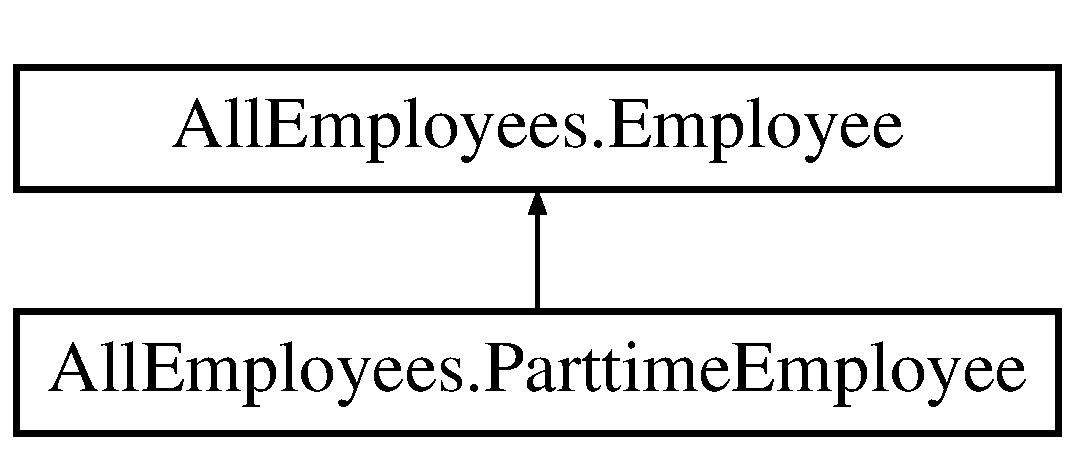
\includegraphics[height=2.000000cm]{class_all_employees_1_1_parttime_employee}
\end{center}
\end{figure}
\subsection*{Public Member Functions}
\begin{DoxyCompactItemize}
\item 
\hyperlink{class_all_employees_1_1_parttime_employee_aefdb20ed1cc9fb007068380a97e3f51e}{Parttime\+Employee} ()
\begin{DoxyCompactList}\small\item\em default constructor. Sets all values to default \end{DoxyCompactList}\item 
\hyperlink{class_all_employees_1_1_parttime_employee_a9c867461dd13baee1e84702999817ffb}{Parttime\+Employee} (string first\+Name, string last\+Name)
\begin{DoxyCompactList}\small\item\em overloaded constructor. Sets name to inputed names, set all other values to default \end{DoxyCompactList}\item 
\hyperlink{class_all_employees_1_1_parttime_employee_a4e465df9dcdecf0ba7eb89eae52d3f3a}{Parttime\+Employee} (string first\+Name, string last\+Name, int social\+Insurance\+Number, Date\+Time date\+Of\+Birth, Date\+Time date\+Of\+Hire, Date\+Time date\+Of\+Termination, float hourly\+Rate)
\begin{DoxyCompactList}\small\item\em overloaded constructor. Sets all values to the values given. no default values \end{DoxyCompactList}\item 
bool \hyperlink{class_all_employees_1_1_parttime_employee_ae9dfe4fa4f371c46c853cb499da663e7}{Validate} ()
\begin{DoxyCompactList}\small\item\em Used to determine in the object contains a valid employee. \end{DoxyCompactList}\item 
string \hyperlink{class_all_employees_1_1_parttime_employee_aab5cb221e05fda2cbac3d3ecb1398595}{Details} ()
\begin{DoxyCompactList}\small\item\em Used to print all employee data to the consol. \end{DoxyCompactList}\item 
override string \hyperlink{class_all_employees_1_1_parttime_employee_ab24493d33b967822f501bd92996a9e21}{To\+String} ()
\begin{DoxyCompactList}\small\item\em Overriden method To\+String used to return a formated string of all data. \end{DoxyCompactList}\item 
bool \hyperlink{class_all_employees_1_1_parttime_employee_a13b87ed00ebf4f834d6c9ff5b3051ca0}{Set\+Date\+Of\+Termination} (Date\+Time date)
\begin{DoxyCompactList}\small\item\em Setter for date\+Of\+Termination. \end{DoxyCompactList}\item 
bool \hyperlink{class_all_employees_1_1_parttime_employee_a305894433e372ba1511999889eebd7f0}{Set\+Date\+Of\+Termination} (string date)
\begin{DoxyCompactList}\small\item\em Setter for date\+Of\+Termination from string. \end{DoxyCompactList}\item 
bool \hyperlink{class_all_employees_1_1_parttime_employee_ad1738c15831d445694a56cf31eaf1e65}{Set\+Date\+Of\+Termination} (int year, int month, int day)
\begin{DoxyCompactList}\small\item\em Setter for date\+Of\+Termination from ints. \end{DoxyCompactList}\item 
bool \hyperlink{class_all_employees_1_1_parttime_employee_a13f02bfe441ed7b6f809f8ed5468bf7f}{Set\+Hourly\+Rate} (float rate)
\begin{DoxyCompactList}\small\item\em Setter for hourly\+Rate. \end{DoxyCompactList}\item 
bool \hyperlink{class_all_employees_1_1_parttime_employee_aa57cd09d4828cb5628f8b6200cdceeac}{Set\+Date\+Of\+Hire} (Date\+Time date)
\begin{DoxyCompactList}\small\item\em Setter for date\+Of\+Hire. \end{DoxyCompactList}\item 
bool \hyperlink{class_all_employees_1_1_parttime_employee_a7b1681699133e08b3c11900b73d757ef}{Set\+Date\+Of\+Hire} (string date)
\begin{DoxyCompactList}\small\item\em Setter for date\+Of\+Hire from string. \end{DoxyCompactList}\item 
bool \hyperlink{class_all_employees_1_1_parttime_employee_a8f49e4626627f95f098c56f092207a8e}{Set\+Date\+Of\+Hire} (int year, int month, int day)
\begin{DoxyCompactList}\small\item\em Setter for date\+Of\+Hire from ints. \end{DoxyCompactList}\item 
Date\+Time \hyperlink{class_all_employees_1_1_parttime_employee_a58fdbd9bf434cfeba1d3418bf1576100}{Get\+Date\+Of\+Termination} ()
\begin{DoxyCompactList}\small\item\em Getter for date\+Of\+Termination. \end{DoxyCompactList}\item 
string \hyperlink{class_all_employees_1_1_parttime_employee_aece6dee0304f86e5d03cb751bd3cbb49}{Get\+Date\+Of\+Termination\+String} ()
\begin{DoxyCompactList}\small\item\em Getter for date\+Of\+Termination that returns formatted string. \end{DoxyCompactList}\item 
float \hyperlink{class_all_employees_1_1_parttime_employee_a05b1fd21f7df07abc013ced6df7959f4}{Get\+Hourly\+Rate} ()
\begin{DoxyCompactList}\small\item\em Getter for hourly\+Rate. \end{DoxyCompactList}\item 
Date\+Time \hyperlink{class_all_employees_1_1_parttime_employee_a266fb09cc25fcf9d5e475d8859b1fdac}{Get\+Date\+Of\+Hire} ()
\begin{DoxyCompactList}\small\item\em Getter for date\+Of\+Hire. \end{DoxyCompactList}\item 
string \hyperlink{class_all_employees_1_1_parttime_employee_a18bd3a43e374b89bdd8f6e2ec9f9e51e}{Get\+Date\+Of\+Hire\+String} ()
\begin{DoxyCompactList}\small\item\em Getter for date\+Of\+Hire that returns formatted string. \end{DoxyCompactList}\end{DoxyCompactItemize}
\subsection*{Private Attributes}
\begin{DoxyCompactItemize}
\item 
\hypertarget{class_all_employees_1_1_parttime_employee_ae9217b6e9531dd5f6ac9029982bab405}{}Date\+Time {\bfseries date\+Of\+Hire}\label{class_all_employees_1_1_parttime_employee_ae9217b6e9531dd5f6ac9029982bab405}

\item 
\hypertarget{class_all_employees_1_1_parttime_employee_a98a60c754150cb7ff049b1a6f9eea5bc}{}Date\+Time {\bfseries date\+Of\+Termination}\label{class_all_employees_1_1_parttime_employee_a98a60c754150cb7ff049b1a6f9eea5bc}

\item 
\hypertarget{class_all_employees_1_1_parttime_employee_abbd98191b1a250e7910012c51f85bcea}{}float {\bfseries hourly\+Rate}\label{class_all_employees_1_1_parttime_employee_abbd98191b1a250e7910012c51f85bcea}

\end{DoxyCompactItemize}
\subsection*{Additional Inherited Members}


\subsection{Detailed Description}
{\bfseries Brief Description} The Parttime \hyperlink{class_all_employees_1_1_employee}{Employee} class is used to store and manage data about a employee who is hired for a part-\/time possition. This class is a child to \hyperlink{class_all_employees_1_1_employee}{Employee} class. It adds the date of hire and termination, and the employees hourly wage. If the constructor creates a invalid employee, a exception is thrown All other errors result in a defined return 

\begin{DoxyAuthor}{Author}
{\itshape Brandon} 
\end{DoxyAuthor}


\subsection{Constructor \& Destructor Documentation}
\hypertarget{class_all_employees_1_1_parttime_employee_aefdb20ed1cc9fb007068380a97e3f51e}{}\index{All\+Employees\+::\+Parttime\+Employee@{All\+Employees\+::\+Parttime\+Employee}!Parttime\+Employee@{Parttime\+Employee}}
\index{Parttime\+Employee@{Parttime\+Employee}!All\+Employees\+::\+Parttime\+Employee@{All\+Employees\+::\+Parttime\+Employee}}
\subsubsection[{Parttime\+Employee}]{\setlength{\rightskip}{0pt plus 5cm}All\+Employees.\+Parttime\+Employee.\+Parttime\+Employee (
\begin{DoxyParamCaption}
{}
\end{DoxyParamCaption}
)}\label{class_all_employees_1_1_parttime_employee_aefdb20ed1cc9fb007068380a97e3f51e}


default constructor. Sets all values to default 

{\bfseries Details}


\begin{DoxyParams}{Parameters}
{\em n/a} & \\
\hline
\end{DoxyParams}
\begin{DoxyReturn}{Returns}
n/a 
\end{DoxyReturn}
\hypertarget{class_all_employees_1_1_parttime_employee_a9c867461dd13baee1e84702999817ffb}{}\index{All\+Employees\+::\+Parttime\+Employee@{All\+Employees\+::\+Parttime\+Employee}!Parttime\+Employee@{Parttime\+Employee}}
\index{Parttime\+Employee@{Parttime\+Employee}!All\+Employees\+::\+Parttime\+Employee@{All\+Employees\+::\+Parttime\+Employee}}
\subsubsection[{Parttime\+Employee}]{\setlength{\rightskip}{0pt plus 5cm}All\+Employees.\+Parttime\+Employee.\+Parttime\+Employee (
\begin{DoxyParamCaption}
\item[{string}]{first\+Name, }
\item[{string}]{last\+Name}
\end{DoxyParamCaption}
)}\label{class_all_employees_1_1_parttime_employee_a9c867461dd13baee1e84702999817ffb}


overloaded constructor. Sets name to inputed names, set all other values to default 

{\bfseries Details}


\begin{DoxyParams}{Parameters}
{\em first\+Name} & -\/ {\bfseries string} -\/ First Name of employee to add to records \\
\hline
{\em last\+Name} & -\/ {\bfseries string} -\/ Last Name of employee to add to records\\
\hline
\end{DoxyParams}

\begin{DoxyExceptions}{Exceptions}
{\em $<$\+Failed\+Constructor\+Exception$>$} & -\/ If the constructor failed to create the object\\
\hline
\end{DoxyExceptions}
\begin{DoxyReturn}{Returns}
n/a 
\end{DoxyReturn}
\hypertarget{class_all_employees_1_1_parttime_employee_a4e465df9dcdecf0ba7eb89eae52d3f3a}{}\index{All\+Employees\+::\+Parttime\+Employee@{All\+Employees\+::\+Parttime\+Employee}!Parttime\+Employee@{Parttime\+Employee}}
\index{Parttime\+Employee@{Parttime\+Employee}!All\+Employees\+::\+Parttime\+Employee@{All\+Employees\+::\+Parttime\+Employee}}
\subsubsection[{Parttime\+Employee}]{\setlength{\rightskip}{0pt plus 5cm}All\+Employees.\+Parttime\+Employee.\+Parttime\+Employee (
\begin{DoxyParamCaption}
\item[{string}]{first\+Name, }
\item[{string}]{last\+Name, }
\item[{int}]{social\+Insurance\+Number, }
\item[{Date\+Time}]{date\+Of\+Birth, }
\item[{Date\+Time}]{date\+Of\+Hire, }
\item[{Date\+Time}]{date\+Of\+Termination, }
\item[{float}]{hourly\+Rate}
\end{DoxyParamCaption}
)}\label{class_all_employees_1_1_parttime_employee_a4e465df9dcdecf0ba7eb89eae52d3f3a}


overloaded constructor. Sets all values to the values given. no default values 

{\bfseries Details}


\begin{DoxyParams}{Parameters}
{\em first\+Name} & -\/ {\bfseries string} -\/ First Name of employee to add to records \\
\hline
{\em last\+Name} & -\/ {\bfseries string} -\/ Last Name of employee to add to records \\
\hline
{\em social\+Insurance\+Number} & -\/ {\bfseries int} -\/ Social Insurance Number of employee to add to records \\
\hline
{\em date\+Of\+Birth} & -\/ {\bfseries Date\+Time} -\/ Date Of Birth of employee to add to records \\
\hline
{\em date\+Of\+Hire} & -\/ {\bfseries Date\+Time} -\/ Date Of Hire of employee to add to records \\
\hline
{\em date\+Of\+Termination} & -\/ {\bfseries Date\+Time} -\/ Date Of Termination of employee to add to records \\
\hline
{\em hourly\+Rate} & -\/ {\bfseries float} -\/ Hourly Rate of employee to add to records\\
\hline
\end{DoxyParams}

\begin{DoxyExceptions}{Exceptions}
{\em $<$\+Failed\+Constructor\+Exception$>$} & -\/ If the constructor failed to create the object\\
\hline
\end{DoxyExceptions}
\begin{DoxyReturn}{Returns}
n/a 
\end{DoxyReturn}


\subsection{Member Function Documentation}
\hypertarget{class_all_employees_1_1_parttime_employee_aab5cb221e05fda2cbac3d3ecb1398595}{}\index{All\+Employees\+::\+Parttime\+Employee@{All\+Employees\+::\+Parttime\+Employee}!Details@{Details}}
\index{Details@{Details}!All\+Employees\+::\+Parttime\+Employee@{All\+Employees\+::\+Parttime\+Employee}}
\subsubsection[{Details}]{\setlength{\rightskip}{0pt plus 5cm}string All\+Employees.\+Parttime\+Employee.\+Details (
\begin{DoxyParamCaption}
{}
\end{DoxyParamCaption}
)}\label{class_all_employees_1_1_parttime_employee_aab5cb221e05fda2cbac3d3ecb1398595}


Used to print all employee data to the consol. 

{\bfseries Details}


\begin{DoxyParams}{Parameters}
{\em n/a} & \\
\hline
\end{DoxyParams}
\begin{DoxyReturn}{Returns}
user\+Info {\bfseries string} -\/ formatted string of employee data 
\end{DoxyReturn}
\hypertarget{class_all_employees_1_1_parttime_employee_a266fb09cc25fcf9d5e475d8859b1fdac}{}\index{All\+Employees\+::\+Parttime\+Employee@{All\+Employees\+::\+Parttime\+Employee}!Get\+Date\+Of\+Hire@{Get\+Date\+Of\+Hire}}
\index{Get\+Date\+Of\+Hire@{Get\+Date\+Of\+Hire}!All\+Employees\+::\+Parttime\+Employee@{All\+Employees\+::\+Parttime\+Employee}}
\subsubsection[{Get\+Date\+Of\+Hire}]{\setlength{\rightskip}{0pt plus 5cm}Date\+Time All\+Employees.\+Parttime\+Employee.\+Get\+Date\+Of\+Hire (
\begin{DoxyParamCaption}
{}
\end{DoxyParamCaption}
)}\label{class_all_employees_1_1_parttime_employee_a266fb09cc25fcf9d5e475d8859b1fdac}


Getter for date\+Of\+Hire. 

{\bfseries Details}


\begin{DoxyParams}{Parameters}
{\em n/a} & \\
\hline
\end{DoxyParams}
\begin{DoxyReturn}{Returns}
date\+Of\+Hire {\bfseries Date\+Time} 
\end{DoxyReturn}
\hypertarget{class_all_employees_1_1_parttime_employee_a18bd3a43e374b89bdd8f6e2ec9f9e51e}{}\index{All\+Employees\+::\+Parttime\+Employee@{All\+Employees\+::\+Parttime\+Employee}!Get\+Date\+Of\+Hire\+String@{Get\+Date\+Of\+Hire\+String}}
\index{Get\+Date\+Of\+Hire\+String@{Get\+Date\+Of\+Hire\+String}!All\+Employees\+::\+Parttime\+Employee@{All\+Employees\+::\+Parttime\+Employee}}
\subsubsection[{Get\+Date\+Of\+Hire\+String}]{\setlength{\rightskip}{0pt plus 5cm}string All\+Employees.\+Parttime\+Employee.\+Get\+Date\+Of\+Hire\+String (
\begin{DoxyParamCaption}
{}
\end{DoxyParamCaption}
)}\label{class_all_employees_1_1_parttime_employee_a18bd3a43e374b89bdd8f6e2ec9f9e51e}


Getter for date\+Of\+Hire that returns formatted string. 

{\bfseries Details}


\begin{DoxyParams}{Parameters}
{\em n/a} & \\
\hline
\end{DoxyParams}
\begin{DoxyReturn}{Returns}
date\+Of\+Hire {\bfseries string} 
\end{DoxyReturn}
\hypertarget{class_all_employees_1_1_parttime_employee_a58fdbd9bf434cfeba1d3418bf1576100}{}\index{All\+Employees\+::\+Parttime\+Employee@{All\+Employees\+::\+Parttime\+Employee}!Get\+Date\+Of\+Termination@{Get\+Date\+Of\+Termination}}
\index{Get\+Date\+Of\+Termination@{Get\+Date\+Of\+Termination}!All\+Employees\+::\+Parttime\+Employee@{All\+Employees\+::\+Parttime\+Employee}}
\subsubsection[{Get\+Date\+Of\+Termination}]{\setlength{\rightskip}{0pt plus 5cm}Date\+Time All\+Employees.\+Parttime\+Employee.\+Get\+Date\+Of\+Termination (
\begin{DoxyParamCaption}
{}
\end{DoxyParamCaption}
)}\label{class_all_employees_1_1_parttime_employee_a58fdbd9bf434cfeba1d3418bf1576100}


Getter for date\+Of\+Termination. 

{\bfseries Details}


\begin{DoxyParams}{Parameters}
{\em n/a} & \\
\hline
\end{DoxyParams}
\begin{DoxyReturn}{Returns}
date\+Of\+Termination {\bfseries Date\+Time} 
\end{DoxyReturn}
\hypertarget{class_all_employees_1_1_parttime_employee_aece6dee0304f86e5d03cb751bd3cbb49}{}\index{All\+Employees\+::\+Parttime\+Employee@{All\+Employees\+::\+Parttime\+Employee}!Get\+Date\+Of\+Termination\+String@{Get\+Date\+Of\+Termination\+String}}
\index{Get\+Date\+Of\+Termination\+String@{Get\+Date\+Of\+Termination\+String}!All\+Employees\+::\+Parttime\+Employee@{All\+Employees\+::\+Parttime\+Employee}}
\subsubsection[{Get\+Date\+Of\+Termination\+String}]{\setlength{\rightskip}{0pt plus 5cm}string All\+Employees.\+Parttime\+Employee.\+Get\+Date\+Of\+Termination\+String (
\begin{DoxyParamCaption}
{}
\end{DoxyParamCaption}
)}\label{class_all_employees_1_1_parttime_employee_aece6dee0304f86e5d03cb751bd3cbb49}


Getter for date\+Of\+Termination that returns formatted string. 

{\bfseries Details}


\begin{DoxyParams}{Parameters}
{\em n/a} & \\
\hline
\end{DoxyParams}
\begin{DoxyReturn}{Returns}
date\+Of\+Termination {\bfseries string} 
\end{DoxyReturn}
\hypertarget{class_all_employees_1_1_parttime_employee_a05b1fd21f7df07abc013ced6df7959f4}{}\index{All\+Employees\+::\+Parttime\+Employee@{All\+Employees\+::\+Parttime\+Employee}!Get\+Hourly\+Rate@{Get\+Hourly\+Rate}}
\index{Get\+Hourly\+Rate@{Get\+Hourly\+Rate}!All\+Employees\+::\+Parttime\+Employee@{All\+Employees\+::\+Parttime\+Employee}}
\subsubsection[{Get\+Hourly\+Rate}]{\setlength{\rightskip}{0pt plus 5cm}float All\+Employees.\+Parttime\+Employee.\+Get\+Hourly\+Rate (
\begin{DoxyParamCaption}
{}
\end{DoxyParamCaption}
)}\label{class_all_employees_1_1_parttime_employee_a05b1fd21f7df07abc013ced6df7959f4}


Getter for hourly\+Rate. 

{\bfseries Details}


\begin{DoxyParams}{Parameters}
{\em n/a} & \\
\hline
\end{DoxyParams}
\begin{DoxyReturn}{Returns}
hourly\+Rate {\bfseries float} 
\end{DoxyReturn}
\hypertarget{class_all_employees_1_1_parttime_employee_aa57cd09d4828cb5628f8b6200cdceeac}{}\index{All\+Employees\+::\+Parttime\+Employee@{All\+Employees\+::\+Parttime\+Employee}!Set\+Date\+Of\+Hire@{Set\+Date\+Of\+Hire}}
\index{Set\+Date\+Of\+Hire@{Set\+Date\+Of\+Hire}!All\+Employees\+::\+Parttime\+Employee@{All\+Employees\+::\+Parttime\+Employee}}
\subsubsection[{Set\+Date\+Of\+Hire}]{\setlength{\rightskip}{0pt plus 5cm}bool All\+Employees.\+Parttime\+Employee.\+Set\+Date\+Of\+Hire (
\begin{DoxyParamCaption}
\item[{Date\+Time}]{date}
\end{DoxyParamCaption}
)}\label{class_all_employees_1_1_parttime_employee_aa57cd09d4828cb5628f8b6200cdceeac}


Setter for date\+Of\+Hire. 

{\bfseries Details}


\begin{DoxyParams}{Parameters}
{\em date} & {\bfseries Date\+Time} -\/ The employees date of hire\\
\hline
\end{DoxyParams}
\begin{DoxyReturn}{Returns}
data\+Saved {\bfseries bool} -\/ true if input was valid and data was changed. False it data was not changed 
\end{DoxyReturn}
\hypertarget{class_all_employees_1_1_parttime_employee_a7b1681699133e08b3c11900b73d757ef}{}\index{All\+Employees\+::\+Parttime\+Employee@{All\+Employees\+::\+Parttime\+Employee}!Set\+Date\+Of\+Hire@{Set\+Date\+Of\+Hire}}
\index{Set\+Date\+Of\+Hire@{Set\+Date\+Of\+Hire}!All\+Employees\+::\+Parttime\+Employee@{All\+Employees\+::\+Parttime\+Employee}}
\subsubsection[{Set\+Date\+Of\+Hire}]{\setlength{\rightskip}{0pt plus 5cm}bool All\+Employees.\+Parttime\+Employee.\+Set\+Date\+Of\+Hire (
\begin{DoxyParamCaption}
\item[{string}]{date}
\end{DoxyParamCaption}
)}\label{class_all_employees_1_1_parttime_employee_a7b1681699133e08b3c11900b73d757ef}


Setter for date\+Of\+Hire from string. 

{\bfseries Details}


\begin{DoxyParams}{Parameters}
{\em date} & {\bfseries string} -\/ The employees date of hire\\
\hline
\end{DoxyParams}
\begin{DoxyReturn}{Returns}
data\+Saved {\bfseries bool} -\/ true if input was valid and data was changed. False it data was not changed 
\end{DoxyReturn}
\hypertarget{class_all_employees_1_1_parttime_employee_a8f49e4626627f95f098c56f092207a8e}{}\index{All\+Employees\+::\+Parttime\+Employee@{All\+Employees\+::\+Parttime\+Employee}!Set\+Date\+Of\+Hire@{Set\+Date\+Of\+Hire}}
\index{Set\+Date\+Of\+Hire@{Set\+Date\+Of\+Hire}!All\+Employees\+::\+Parttime\+Employee@{All\+Employees\+::\+Parttime\+Employee}}
\subsubsection[{Set\+Date\+Of\+Hire}]{\setlength{\rightskip}{0pt plus 5cm}bool All\+Employees.\+Parttime\+Employee.\+Set\+Date\+Of\+Hire (
\begin{DoxyParamCaption}
\item[{int}]{year, }
\item[{int}]{month, }
\item[{int}]{day}
\end{DoxyParamCaption}
)}\label{class_all_employees_1_1_parttime_employee_a8f49e4626627f95f098c56f092207a8e}


Setter for date\+Of\+Hire from ints. 

{\bfseries Details}


\begin{DoxyParams}{Parameters}
{\em year} & {\bfseries int} -\/ The year of the employees date\+Of\+Hire \\
\hline
{\em month} & {\bfseries int} -\/ The month of the employees date\+Of\+Hire \\
\hline
{\em day} & {\bfseries int} -\/ The day of the employees date\+Of\+Hire\\
\hline
\end{DoxyParams}
\begin{DoxyReturn}{Returns}
data\+Saved {\bfseries bool} -\/ true if input was valid and data was changed. False it data was not changed 
\end{DoxyReturn}
\hypertarget{class_all_employees_1_1_parttime_employee_a13b87ed00ebf4f834d6c9ff5b3051ca0}{}\index{All\+Employees\+::\+Parttime\+Employee@{All\+Employees\+::\+Parttime\+Employee}!Set\+Date\+Of\+Termination@{Set\+Date\+Of\+Termination}}
\index{Set\+Date\+Of\+Termination@{Set\+Date\+Of\+Termination}!All\+Employees\+::\+Parttime\+Employee@{All\+Employees\+::\+Parttime\+Employee}}
\subsubsection[{Set\+Date\+Of\+Termination}]{\setlength{\rightskip}{0pt plus 5cm}bool All\+Employees.\+Parttime\+Employee.\+Set\+Date\+Of\+Termination (
\begin{DoxyParamCaption}
\item[{Date\+Time}]{date}
\end{DoxyParamCaption}
)}\label{class_all_employees_1_1_parttime_employee_a13b87ed00ebf4f834d6c9ff5b3051ca0}


Setter for date\+Of\+Termination. 

{\bfseries Details}


\begin{DoxyParams}{Parameters}
{\em date} & {\bfseries Date\+Time} -\/ The employees date of termination\\
\hline
\end{DoxyParams}
\begin{DoxyReturn}{Returns}
data\+Saved {\bfseries bool} -\/ true if input was valid and data was changed. False it data was not changed 
\end{DoxyReturn}
\hypertarget{class_all_employees_1_1_parttime_employee_a305894433e372ba1511999889eebd7f0}{}\index{All\+Employees\+::\+Parttime\+Employee@{All\+Employees\+::\+Parttime\+Employee}!Set\+Date\+Of\+Termination@{Set\+Date\+Of\+Termination}}
\index{Set\+Date\+Of\+Termination@{Set\+Date\+Of\+Termination}!All\+Employees\+::\+Parttime\+Employee@{All\+Employees\+::\+Parttime\+Employee}}
\subsubsection[{Set\+Date\+Of\+Termination}]{\setlength{\rightskip}{0pt plus 5cm}bool All\+Employees.\+Parttime\+Employee.\+Set\+Date\+Of\+Termination (
\begin{DoxyParamCaption}
\item[{string}]{date}
\end{DoxyParamCaption}
)}\label{class_all_employees_1_1_parttime_employee_a305894433e372ba1511999889eebd7f0}


Setter for date\+Of\+Termination from string. 

{\bfseries Details}


\begin{DoxyParams}{Parameters}
{\em date} & {\bfseries string} -\/ The employees date of termination\\
\hline
\end{DoxyParams}
\begin{DoxyReturn}{Returns}
data\+Saved {\bfseries bool} -\/ true if input was valid and data was changed. False it data was not changed 
\end{DoxyReturn}
\hypertarget{class_all_employees_1_1_parttime_employee_ad1738c15831d445694a56cf31eaf1e65}{}\index{All\+Employees\+::\+Parttime\+Employee@{All\+Employees\+::\+Parttime\+Employee}!Set\+Date\+Of\+Termination@{Set\+Date\+Of\+Termination}}
\index{Set\+Date\+Of\+Termination@{Set\+Date\+Of\+Termination}!All\+Employees\+::\+Parttime\+Employee@{All\+Employees\+::\+Parttime\+Employee}}
\subsubsection[{Set\+Date\+Of\+Termination}]{\setlength{\rightskip}{0pt plus 5cm}bool All\+Employees.\+Parttime\+Employee.\+Set\+Date\+Of\+Termination (
\begin{DoxyParamCaption}
\item[{int}]{year, }
\item[{int}]{month, }
\item[{int}]{day}
\end{DoxyParamCaption}
)}\label{class_all_employees_1_1_parttime_employee_ad1738c15831d445694a56cf31eaf1e65}


Setter for date\+Of\+Termination from ints. 

{\bfseries Details}


\begin{DoxyParams}{Parameters}
{\em year} & {\bfseries int} -\/ The year of the employees Termination \\
\hline
{\em month} & {\bfseries int} -\/ The month of the employees Termination \\
\hline
{\em day} & {\bfseries int} -\/ The day of the employees Termination\\
\hline
\end{DoxyParams}
\begin{DoxyReturn}{Returns}
data\+Saved {\bfseries bool} -\/ true if input was valid and data was changed. False it data was not changed 
\end{DoxyReturn}
\hypertarget{class_all_employees_1_1_parttime_employee_a13f02bfe441ed7b6f809f8ed5468bf7f}{}\index{All\+Employees\+::\+Parttime\+Employee@{All\+Employees\+::\+Parttime\+Employee}!Set\+Hourly\+Rate@{Set\+Hourly\+Rate}}
\index{Set\+Hourly\+Rate@{Set\+Hourly\+Rate}!All\+Employees\+::\+Parttime\+Employee@{All\+Employees\+::\+Parttime\+Employee}}
\subsubsection[{Set\+Hourly\+Rate}]{\setlength{\rightskip}{0pt plus 5cm}bool All\+Employees.\+Parttime\+Employee.\+Set\+Hourly\+Rate (
\begin{DoxyParamCaption}
\item[{float}]{rate}
\end{DoxyParamCaption}
)}\label{class_all_employees_1_1_parttime_employee_a13f02bfe441ed7b6f809f8ed5468bf7f}


Setter for hourly\+Rate. 

{\bfseries Details}


\begin{DoxyParams}{Parameters}
{\em rate} & {\bfseries float} -\/ The employees hourly rate\\
\hline
\end{DoxyParams}
\begin{DoxyReturn}{Returns}
data\+Saved {\bfseries bool} -\/ true if input was valid and data was changed. False it data was not changed 
\end{DoxyReturn}
\hypertarget{class_all_employees_1_1_parttime_employee_ab24493d33b967822f501bd92996a9e21}{}\index{All\+Employees\+::\+Parttime\+Employee@{All\+Employees\+::\+Parttime\+Employee}!To\+String@{To\+String}}
\index{To\+String@{To\+String}!All\+Employees\+::\+Parttime\+Employee@{All\+Employees\+::\+Parttime\+Employee}}
\subsubsection[{To\+String}]{\setlength{\rightskip}{0pt plus 5cm}override string All\+Employees.\+Parttime\+Employee.\+To\+String (
\begin{DoxyParamCaption}
{}
\end{DoxyParamCaption}
)}\label{class_all_employees_1_1_parttime_employee_ab24493d33b967822f501bd92996a9e21}


Overriden method To\+String used to return a formated string of all data. 

{\bfseries Details}


\begin{DoxyParams}{Parameters}
{\em n/a} & \\
\hline
\end{DoxyParams}
\begin{DoxyReturn}{Returns}
employee\+String {\bfseries string} -\/ the formated string containing all employee data 
\end{DoxyReturn}
\hypertarget{class_all_employees_1_1_parttime_employee_ae9dfe4fa4f371c46c853cb499da663e7}{}\index{All\+Employees\+::\+Parttime\+Employee@{All\+Employees\+::\+Parttime\+Employee}!Validate@{Validate}}
\index{Validate@{Validate}!All\+Employees\+::\+Parttime\+Employee@{All\+Employees\+::\+Parttime\+Employee}}
\subsubsection[{Validate}]{\setlength{\rightskip}{0pt plus 5cm}bool All\+Employees.\+Parttime\+Employee.\+Validate (
\begin{DoxyParamCaption}
{}
\end{DoxyParamCaption}
)}\label{class_all_employees_1_1_parttime_employee_ae9dfe4fa4f371c46c853cb499da663e7}


Used to determine in the object contains a valid employee. 

{\bfseries Details}


\begin{DoxyParams}{Parameters}
{\em n/a} & \\
\hline
\end{DoxyParams}
\begin{DoxyReturn}{Returns}
data\+Valid -\/ {\bfseries bool} -\/ True if the object contains all data for a valid employee 
\end{DoxyReturn}


The documentation for this class was generated from the following file\+:\begin{DoxyCompactItemize}
\item 
C\+:/\+S\+E\+T\+Repo/trunk/\+E\+M\+S/trunk/\+All\+Employees/\+All\+Employees/Parttime\+Employee.\+cs\end{DoxyCompactItemize}

\hypertarget{class_all_employees_1_1_seasonal_employee}{}\section{All\+Employees.\+Seasonal\+Employee Class Reference}
\label{class_all_employees_1_1_seasonal_employee}\index{All\+Employees.\+Seasonal\+Employee@{All\+Employees.\+Seasonal\+Employee}}


{\bfseries Brief Description} The Seasonal \hyperlink{class_all_employees_1_1_employee}{Employee} class is used to store and manage data about a employee who is hired for a season. This class is a child to \hyperlink{class_all_employees_1_1_employee}{Employee} class. It adds the season the employee is hired for and how much the employee is paid per item completed/created.  


Inheritance diagram for All\+Employees.\+Seasonal\+Employee\+:\begin{figure}[H]
\begin{center}
\leavevmode
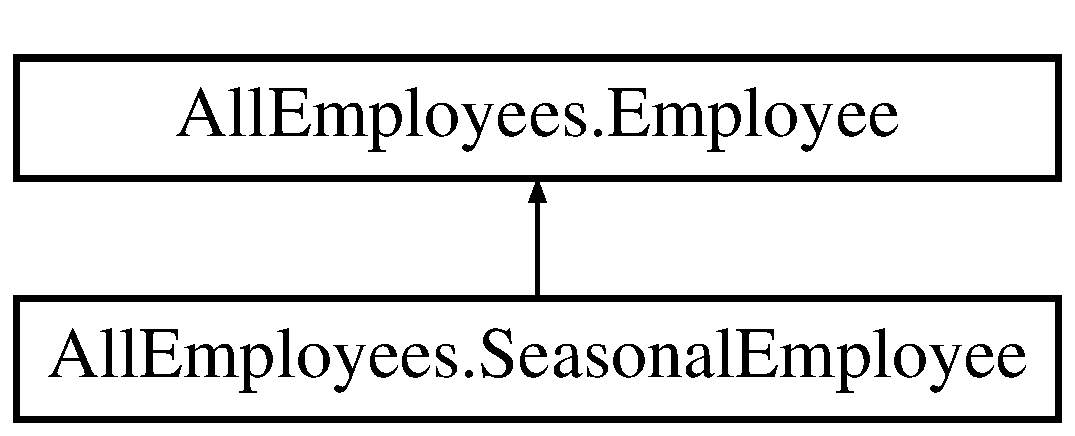
\includegraphics[height=2.000000cm]{class_all_employees_1_1_seasonal_employee}
\end{center}
\end{figure}
\subsection*{Public Member Functions}
\begin{DoxyCompactItemize}
\item 
\hyperlink{class_all_employees_1_1_seasonal_employee_a2206a19da96d42cbd56e7fb5d073c7d4}{Seasonal\+Employee} ()
\begin{DoxyCompactList}\small\item\em default constructor. Sets all values to default \end{DoxyCompactList}\item 
\hyperlink{class_all_employees_1_1_seasonal_employee_acc7fb6022faa7594a0e249a8ba89f217}{Seasonal\+Employee} (string first\+Name, string last\+Name)
\begin{DoxyCompactList}\small\item\em overloaded constructor. Sets name to inputed names, set all other values to default \end{DoxyCompactList}\item 
\hyperlink{class_all_employees_1_1_seasonal_employee_a11c78ec2f72bdeb29d71d48497e34c63}{Seasonal\+Employee} (string first\+Name, string last\+Name, int social\+Insurance\+Number, Date\+Time date\+Of\+Birth, string season, float piece\+Pay)
\begin{DoxyCompactList}\small\item\em overloaded constructor. Sets all values to the values given. no default values \end{DoxyCompactList}\item 
bool \hyperlink{class_all_employees_1_1_seasonal_employee_a70f911ac43a67b84f93ead74860bb6d9}{Validate} ()
\begin{DoxyCompactList}\small\item\em Used to determine in the object contains a valid employee. \end{DoxyCompactList}\item 
string \hyperlink{class_all_employees_1_1_seasonal_employee_a0474e4afe0e11f4e2dd0a523bff3034b}{Details} ()
\begin{DoxyCompactList}\small\item\em Used to print all employee data to the consol. \end{DoxyCompactList}\item 
override string \hyperlink{class_all_employees_1_1_seasonal_employee_a797da83b3ef0a5e7fb04fc5b0d373a11}{To\+String} ()
\begin{DoxyCompactList}\small\item\em Overriden method To\+String used to return a formated string of all data. \end{DoxyCompactList}\item 
bool \hyperlink{class_all_employees_1_1_seasonal_employee_a3cefc2899365780dd013b990ef46326c}{Set\+Season} (string season)
\begin{DoxyCompactList}\small\item\em Setter for season. \end{DoxyCompactList}\item 
bool \hyperlink{class_all_employees_1_1_seasonal_employee_a983e9f6a2a1fd71ed056d8b50d787e88}{Set\+Piece\+Pay} (float piece\+Pay)
\begin{DoxyCompactList}\small\item\em Setter for piece\+Pay. \end{DoxyCompactList}\item 
string \hyperlink{class_all_employees_1_1_seasonal_employee_a189a882ddc11648f3df82e5c0acd5522}{Get\+Season} ()
\begin{DoxyCompactList}\small\item\em Getter for season. \end{DoxyCompactList}\item 
float \hyperlink{class_all_employees_1_1_seasonal_employee_ae7836e968d20baba7327577807d36aa7}{Get\+Piece\+Pay} ()
\begin{DoxyCompactList}\small\item\em Getter for piece\+Pay. \end{DoxyCompactList}\end{DoxyCompactItemize}
\subsection*{Private Attributes}
\begin{DoxyCompactItemize}
\item 
\hypertarget{class_all_employees_1_1_seasonal_employee_a7615ccd677faed6b26afa27aadd7a71e}{}string {\bfseries season}\label{class_all_employees_1_1_seasonal_employee_a7615ccd677faed6b26afa27aadd7a71e}

\item 
\hypertarget{class_all_employees_1_1_seasonal_employee_afc65d49c016c4510e123b93c9570b639}{}float {\bfseries piece\+Pay}\label{class_all_employees_1_1_seasonal_employee_afc65d49c016c4510e123b93c9570b639}

\end{DoxyCompactItemize}
\subsection*{Additional Inherited Members}


\subsection{Detailed Description}
{\bfseries Brief Description} The Seasonal \hyperlink{class_all_employees_1_1_employee}{Employee} class is used to store and manage data about a employee who is hired for a season. This class is a child to \hyperlink{class_all_employees_1_1_employee}{Employee} class. It adds the season the employee is hired for and how much the employee is paid per item completed/created. 

\begin{DoxyAuthor}{Author}
{\itshape Brandon} 
\end{DoxyAuthor}


\subsection{Constructor \& Destructor Documentation}
\hypertarget{class_all_employees_1_1_seasonal_employee_a2206a19da96d42cbd56e7fb5d073c7d4}{}\index{All\+Employees\+::\+Seasonal\+Employee@{All\+Employees\+::\+Seasonal\+Employee}!Seasonal\+Employee@{Seasonal\+Employee}}
\index{Seasonal\+Employee@{Seasonal\+Employee}!All\+Employees\+::\+Seasonal\+Employee@{All\+Employees\+::\+Seasonal\+Employee}}
\subsubsection[{Seasonal\+Employee}]{\setlength{\rightskip}{0pt plus 5cm}All\+Employees.\+Seasonal\+Employee.\+Seasonal\+Employee (
\begin{DoxyParamCaption}
{}
\end{DoxyParamCaption}
)}\label{class_all_employees_1_1_seasonal_employee_a2206a19da96d42cbd56e7fb5d073c7d4}


default constructor. Sets all values to default 

{\bfseries Details}


\begin{DoxyParams}{Parameters}
{\em n/a} & \\
\hline
\end{DoxyParams}
\begin{DoxyReturn}{Returns}
n/a 
\end{DoxyReturn}
\hypertarget{class_all_employees_1_1_seasonal_employee_acc7fb6022faa7594a0e249a8ba89f217}{}\index{All\+Employees\+::\+Seasonal\+Employee@{All\+Employees\+::\+Seasonal\+Employee}!Seasonal\+Employee@{Seasonal\+Employee}}
\index{Seasonal\+Employee@{Seasonal\+Employee}!All\+Employees\+::\+Seasonal\+Employee@{All\+Employees\+::\+Seasonal\+Employee}}
\subsubsection[{Seasonal\+Employee}]{\setlength{\rightskip}{0pt plus 5cm}All\+Employees.\+Seasonal\+Employee.\+Seasonal\+Employee (
\begin{DoxyParamCaption}
\item[{string}]{first\+Name, }
\item[{string}]{last\+Name}
\end{DoxyParamCaption}
)}\label{class_all_employees_1_1_seasonal_employee_acc7fb6022faa7594a0e249a8ba89f217}


overloaded constructor. Sets name to inputed names, set all other values to default 

{\bfseries Details}


\begin{DoxyParams}{Parameters}
{\em first\+Name} & -\/ {\bfseries string} -\/ First Name of employee to add to records \\
\hline
{\em last\+Name} & -\/ {\bfseries string} -\/ Last Name of employee to add to records\\
\hline
\end{DoxyParams}

\begin{DoxyExceptions}{Exceptions}
{\em $<$\+Failed\+Constructor\+Exception$>$} & -\/ If the constructor failed to create the object\\
\hline
\end{DoxyExceptions}
\begin{DoxyReturn}{Returns}
n/a 
\end{DoxyReturn}
\hypertarget{class_all_employees_1_1_seasonal_employee_a11c78ec2f72bdeb29d71d48497e34c63}{}\index{All\+Employees\+::\+Seasonal\+Employee@{All\+Employees\+::\+Seasonal\+Employee}!Seasonal\+Employee@{Seasonal\+Employee}}
\index{Seasonal\+Employee@{Seasonal\+Employee}!All\+Employees\+::\+Seasonal\+Employee@{All\+Employees\+::\+Seasonal\+Employee}}
\subsubsection[{Seasonal\+Employee}]{\setlength{\rightskip}{0pt plus 5cm}All\+Employees.\+Seasonal\+Employee.\+Seasonal\+Employee (
\begin{DoxyParamCaption}
\item[{string}]{first\+Name, }
\item[{string}]{last\+Name, }
\item[{int}]{social\+Insurance\+Number, }
\item[{Date\+Time}]{date\+Of\+Birth, }
\item[{string}]{season, }
\item[{float}]{piece\+Pay}
\end{DoxyParamCaption}
)}\label{class_all_employees_1_1_seasonal_employee_a11c78ec2f72bdeb29d71d48497e34c63}


overloaded constructor. Sets all values to the values given. no default values 

{\bfseries Details}


\begin{DoxyParams}{Parameters}
{\em first\+Name} & -\/ {\bfseries string} -\/ First Name of employee to add to records \\
\hline
{\em last\+Name} & -\/ {\bfseries string} -\/ Last Name of employee to add to records \\
\hline
{\em social\+Insurance\+Number} & -\/ {\bfseries int} -\/ Social Insurance Number of employee to add to records \\
\hline
{\em date\+Of\+Birth} & -\/ {\bfseries Date\+Time} -\/ Date Of Birth of employee to add to records \\
\hline
{\em season} & -\/ {\bfseries string} -\/ season the employee worked/works \\
\hline
{\em piece\+Pay} & -\/ {\bfseries float} -\/ the price per unit that the worker is payed\\
\hline
\end{DoxyParams}

\begin{DoxyExceptions}{Exceptions}
{\em $<$\+Failed\+Constructor\+Exception$>$} & -\/ If the constructor failed to create the object\\
\hline
\end{DoxyExceptions}
\begin{DoxyReturn}{Returns}
n/a 
\end{DoxyReturn}


\subsection{Member Function Documentation}
\hypertarget{class_all_employees_1_1_seasonal_employee_a0474e4afe0e11f4e2dd0a523bff3034b}{}\index{All\+Employees\+::\+Seasonal\+Employee@{All\+Employees\+::\+Seasonal\+Employee}!Details@{Details}}
\index{Details@{Details}!All\+Employees\+::\+Seasonal\+Employee@{All\+Employees\+::\+Seasonal\+Employee}}
\subsubsection[{Details}]{\setlength{\rightskip}{0pt plus 5cm}string All\+Employees.\+Seasonal\+Employee.\+Details (
\begin{DoxyParamCaption}
{}
\end{DoxyParamCaption}
)}\label{class_all_employees_1_1_seasonal_employee_a0474e4afe0e11f4e2dd0a523bff3034b}


Used to print all employee data to the consol. 

{\bfseries Details}


\begin{DoxyParams}{Parameters}
{\em n/a} & \\
\hline
\end{DoxyParams}
\begin{DoxyReturn}{Returns}
user\+Info {\bfseries string} -\/ formatted string of employee data 
\end{DoxyReturn}
\hypertarget{class_all_employees_1_1_seasonal_employee_ae7836e968d20baba7327577807d36aa7}{}\index{All\+Employees\+::\+Seasonal\+Employee@{All\+Employees\+::\+Seasonal\+Employee}!Get\+Piece\+Pay@{Get\+Piece\+Pay}}
\index{Get\+Piece\+Pay@{Get\+Piece\+Pay}!All\+Employees\+::\+Seasonal\+Employee@{All\+Employees\+::\+Seasonal\+Employee}}
\subsubsection[{Get\+Piece\+Pay}]{\setlength{\rightskip}{0pt plus 5cm}float All\+Employees.\+Seasonal\+Employee.\+Get\+Piece\+Pay (
\begin{DoxyParamCaption}
{}
\end{DoxyParamCaption}
)}\label{class_all_employees_1_1_seasonal_employee_ae7836e968d20baba7327577807d36aa7}


Getter for piece\+Pay. 

{\bfseries Details}


\begin{DoxyParams}{Parameters}
{\em n/a} & \\
\hline
\end{DoxyParams}
\begin{DoxyReturn}{Returns}
piece\+Pay {\bfseries float} 
\end{DoxyReturn}
\hypertarget{class_all_employees_1_1_seasonal_employee_a189a882ddc11648f3df82e5c0acd5522}{}\index{All\+Employees\+::\+Seasonal\+Employee@{All\+Employees\+::\+Seasonal\+Employee}!Get\+Season@{Get\+Season}}
\index{Get\+Season@{Get\+Season}!All\+Employees\+::\+Seasonal\+Employee@{All\+Employees\+::\+Seasonal\+Employee}}
\subsubsection[{Get\+Season}]{\setlength{\rightskip}{0pt plus 5cm}string All\+Employees.\+Seasonal\+Employee.\+Get\+Season (
\begin{DoxyParamCaption}
{}
\end{DoxyParamCaption}
)}\label{class_all_employees_1_1_seasonal_employee_a189a882ddc11648f3df82e5c0acd5522}


Getter for season. 

{\bfseries Details}


\begin{DoxyParams}{Parameters}
{\em n/a} & \\
\hline
\end{DoxyParams}
\begin{DoxyReturn}{Returns}
season {\bfseries string} 
\end{DoxyReturn}
\hypertarget{class_all_employees_1_1_seasonal_employee_a983e9f6a2a1fd71ed056d8b50d787e88}{}\index{All\+Employees\+::\+Seasonal\+Employee@{All\+Employees\+::\+Seasonal\+Employee}!Set\+Piece\+Pay@{Set\+Piece\+Pay}}
\index{Set\+Piece\+Pay@{Set\+Piece\+Pay}!All\+Employees\+::\+Seasonal\+Employee@{All\+Employees\+::\+Seasonal\+Employee}}
\subsubsection[{Set\+Piece\+Pay}]{\setlength{\rightskip}{0pt plus 5cm}bool All\+Employees.\+Seasonal\+Employee.\+Set\+Piece\+Pay (
\begin{DoxyParamCaption}
\item[{float}]{piece\+Pay}
\end{DoxyParamCaption}
)}\label{class_all_employees_1_1_seasonal_employee_a983e9f6a2a1fd71ed056d8b50d787e88}


Setter for piece\+Pay. 

{\bfseries Details}


\begin{DoxyParams}{Parameters}
{\em piece\+Pay} & {\bfseries float} -\/ The price the employee is payed for each unit created\\
\hline
\end{DoxyParams}
\begin{DoxyReturn}{Returns}
data\+Saved {\bfseries bool} -\/ true if input was valid and data was changed. False it data was not changed 
\end{DoxyReturn}
\hypertarget{class_all_employees_1_1_seasonal_employee_a3cefc2899365780dd013b990ef46326c}{}\index{All\+Employees\+::\+Seasonal\+Employee@{All\+Employees\+::\+Seasonal\+Employee}!Set\+Season@{Set\+Season}}
\index{Set\+Season@{Set\+Season}!All\+Employees\+::\+Seasonal\+Employee@{All\+Employees\+::\+Seasonal\+Employee}}
\subsubsection[{Set\+Season}]{\setlength{\rightskip}{0pt plus 5cm}bool All\+Employees.\+Seasonal\+Employee.\+Set\+Season (
\begin{DoxyParamCaption}
\item[{string}]{season}
\end{DoxyParamCaption}
)}\label{class_all_employees_1_1_seasonal_employee_a3cefc2899365780dd013b990ef46326c}


Setter for season. 

{\bfseries Details}


\begin{DoxyParams}{Parameters}
{\em season} & {\bfseries string} -\/ The season the employee worked/works in\\
\hline
\end{DoxyParams}
\begin{DoxyReturn}{Returns}
data\+Saved {\bfseries bool} -\/ true if input was valid and data was changed. False it data was not changed 
\end{DoxyReturn}
\hypertarget{class_all_employees_1_1_seasonal_employee_a797da83b3ef0a5e7fb04fc5b0d373a11}{}\index{All\+Employees\+::\+Seasonal\+Employee@{All\+Employees\+::\+Seasonal\+Employee}!To\+String@{To\+String}}
\index{To\+String@{To\+String}!All\+Employees\+::\+Seasonal\+Employee@{All\+Employees\+::\+Seasonal\+Employee}}
\subsubsection[{To\+String}]{\setlength{\rightskip}{0pt plus 5cm}override string All\+Employees.\+Seasonal\+Employee.\+To\+String (
\begin{DoxyParamCaption}
{}
\end{DoxyParamCaption}
)}\label{class_all_employees_1_1_seasonal_employee_a797da83b3ef0a5e7fb04fc5b0d373a11}


Overriden method To\+String used to return a formated string of all data. 

{\bfseries Details}


\begin{DoxyParams}{Parameters}
{\em n/a} & \\
\hline
\end{DoxyParams}
\begin{DoxyReturn}{Returns}
employee\+String {\bfseries string} -\/ the formated string containing all employee data 
\end{DoxyReturn}
\hypertarget{class_all_employees_1_1_seasonal_employee_a70f911ac43a67b84f93ead74860bb6d9}{}\index{All\+Employees\+::\+Seasonal\+Employee@{All\+Employees\+::\+Seasonal\+Employee}!Validate@{Validate}}
\index{Validate@{Validate}!All\+Employees\+::\+Seasonal\+Employee@{All\+Employees\+::\+Seasonal\+Employee}}
\subsubsection[{Validate}]{\setlength{\rightskip}{0pt plus 5cm}bool All\+Employees.\+Seasonal\+Employee.\+Validate (
\begin{DoxyParamCaption}
{}
\end{DoxyParamCaption}
)}\label{class_all_employees_1_1_seasonal_employee_a70f911ac43a67b84f93ead74860bb6d9}


Used to determine in the object contains a valid employee. 

{\bfseries Details}


\begin{DoxyParams}{Parameters}
{\em n/a} & \\
\hline
\end{DoxyParams}
\begin{DoxyReturn}{Returns}
data\+Valid -\/ {\bfseries bool} -\/ True if the object contains all data for a valid employee 
\end{DoxyReturn}


The documentation for this class was generated from the following file\+:\begin{DoxyCompactItemize}
\item 
C\+:/\+S\+E\+T\+Repo/trunk/\+E\+M\+S/trunk/\+All\+Employees/\+All\+Employees/Seasonal\+Employee.\+cs\end{DoxyCompactItemize}

\hypertarget{class_presentation_1_1_u_i_menu}{}\section{Presentation.\+U\+I\+Menu Class Reference}
\label{class_presentation_1_1_u_i_menu}\index{Presentation.\+U\+I\+Menu@{Presentation.\+U\+I\+Menu}}


{\bfseries Brief Description} -\/ This class dislays to the user a number of menus where the user then can access the database and either insert, delete, or make changes. If the user inputs don\textquotesingle{}t match up to what is acceptable, the user will be notified appropriately.  


\subsection*{Public Member Functions}
\begin{DoxyCompactItemize}
\item 
\hyperlink{class_presentation_1_1_u_i_menu_aecce7fd9ed4696929cbcada2da8c4c2c}{U\+I\+Menu} ()
\begin{DoxyCompactList}\small\item\em The \hyperlink{class_presentation_1_1_u_i_menu}{U\+I\+Menu} constructor sets up a Container object to be used throughout the page. \end{DoxyCompactList}\item 
\hyperlink{class_presentation_1_1_u_i_menu_ac27724c06cbdcddbcf940f812ba307e3}{U\+I\+Menu} (\hyperlink{class_the_company_1_1_container}{Container} repo)
\begin{DoxyCompactList}\small\item\em The \hyperlink{class_presentation_1_1_u_i_menu}{U\+I\+Menu} constructor connects Container object to the repo. \end{DoxyCompactList}\item 
bool \hyperlink{class_presentation_1_1_u_i_menu_aa358c475a580c724b992458425649ada}{Show\+Main\+Menu} ()
\begin{DoxyCompactList}\small\item\em The Show\+Main\+Menu method will display to the user, a U\+I menu.\+This menu allows the user to choose either to manage E\+M\+S database files, manage employees, or to quit the program. \end{DoxyCompactList}\end{DoxyCompactItemize}
\subsection*{Static Public Member Functions}
\begin{DoxyCompactItemize}
\item 
static \hyperlink{class_all_employees_1_1_employee}{All\+Employees.\+Employee} \hyperlink{class_presentation_1_1_u_i_menu_a02eeec49ff4b872dd3a2cc919ea958c1}{Show\+Find\+Employee\+Menu} ()
\begin{DoxyCompactList}\small\item\em The Show\+Find\+Employee\+Menu method will display to the user, a U\+I menu.\+This menu allows the user to search for a specific employee in the database. \end{DoxyCompactList}\item 
static String \hyperlink{class_presentation_1_1_u_i_menu_a501cb74c71850dc68b255ff502449031}{Get\+Info\+From\+User} (String User\+Prompt)
\begin{DoxyCompactList}\small\item\em The Get\+Info\+From\+User method will get the users input and return it to further process it. \end{DoxyCompactList}\item 
static void \hyperlink{class_presentation_1_1_u_i_menu_a8e46eecdb65e045345059e8a8a44c216}{Show\+Error} (String error\+Message)
\begin{DoxyCompactList}\small\item\em The Show\+Error method displays an appropriate error message to the user. \end{DoxyCompactList}\end{DoxyCompactItemize}
\subsection*{Private Member Functions}
\begin{DoxyCompactItemize}
\item 
void \hyperlink{class_presentation_1_1_u_i_menu_aae74bf481ca23465073a4fbe0b02ee42}{Show\+File\+Management\+Menu} ()
\begin{DoxyCompactList}\small\item\em The Show\+File\+Management\+Menu method will display to the user, a U\+I menu.\+This menu allows the user to choose either to load the E\+M\+S database from the file, save an employee set to the E\+M\+S database, or return to the main menu. \end{DoxyCompactList}\item 
void \hyperlink{class_presentation_1_1_u_i_menu_a2755275ac6f0b154a342ea70d2acf6d1}{Show\+Employee\+Management\+Menu} ()
\begin{DoxyCompactList}\small\item\em The Show\+Employee\+Management\+Menu method will display to the user, a U\+I menu.\+This menu allows the user to choose either to display an employee set, create a new employee, modify and exisiting employee, remove an existing employee, or return to the main menu. \end{DoxyCompactList}\item 
void \hyperlink{class_presentation_1_1_u_i_menu_ab97bfee80ea2bd9d971fba3e79d3b775}{Show\+Employee\+Details\+Menu} ()
\begin{DoxyCompactList}\small\item\em The Show\+Employee\+Details\+Menu method will display to the user, a U\+I menu.\+This menu allows the user to choose either to specify base employee details, to specify values for any employee type, or return to the employee management menu. \end{DoxyCompactList}\end{DoxyCompactItemize}
\subsection*{Private Attributes}
\begin{DoxyCompactItemize}
\item 
\hypertarget{class_presentation_1_1_u_i_menu_ada9168d7b009f78447aa7e748d160585}{}\hyperlink{class_the_company_1_1_container}{Container} {\bfseries company}\label{class_presentation_1_1_u_i_menu_ada9168d7b009f78447aa7e748d160585}

\end{DoxyCompactItemize}


\subsection{Detailed Description}
{\bfseries Brief Description} -\/ This class dislays to the user a number of menus where the user then can access the database and either insert, delete, or make changes. If the user inputs don\textquotesingle{}t match up to what is acceptable, the user will be notified appropriately. 

\begin{DoxyAuthor}{Author}
{\itshape Jennifer Klimova} 
\end{DoxyAuthor}


\subsection{Constructor \& Destructor Documentation}
\hypertarget{class_presentation_1_1_u_i_menu_aecce7fd9ed4696929cbcada2da8c4c2c}{}\index{Presentation\+::\+U\+I\+Menu@{Presentation\+::\+U\+I\+Menu}!U\+I\+Menu@{U\+I\+Menu}}
\index{U\+I\+Menu@{U\+I\+Menu}!Presentation\+::\+U\+I\+Menu@{Presentation\+::\+U\+I\+Menu}}
\subsubsection[{U\+I\+Menu}]{\setlength{\rightskip}{0pt plus 5cm}Presentation.\+U\+I\+Menu.\+U\+I\+Menu (
\begin{DoxyParamCaption}
{}
\end{DoxyParamCaption}
)}\label{class_presentation_1_1_u_i_menu_aecce7fd9ed4696929cbcada2da8c4c2c}


The \hyperlink{class_presentation_1_1_u_i_menu}{U\+I\+Menu} constructor sets up a Container object to be used throughout the page. 

{\bfseries Details}


\begin{DoxyParams}{Parameters}
{\em args} & -\/ n/a\\
\hline
\end{DoxyParams}

\begin{DoxyExceptions}{Exceptions}
{\em $<$\+End\+Of\+Program\+Exception$>$} & -\/ If the user wants the program to end\\
\hline
\end{DoxyExceptions}
\begin{DoxyReturn}{Returns}
n/a 
\end{DoxyReturn}
\hypertarget{class_presentation_1_1_u_i_menu_ac27724c06cbdcddbcf940f812ba307e3}{}\index{Presentation\+::\+U\+I\+Menu@{Presentation\+::\+U\+I\+Menu}!U\+I\+Menu@{U\+I\+Menu}}
\index{U\+I\+Menu@{U\+I\+Menu}!Presentation\+::\+U\+I\+Menu@{Presentation\+::\+U\+I\+Menu}}
\subsubsection[{U\+I\+Menu}]{\setlength{\rightskip}{0pt plus 5cm}Presentation.\+U\+I\+Menu.\+U\+I\+Menu (
\begin{DoxyParamCaption}
\item[{{\bf Container}}]{repo}
\end{DoxyParamCaption}
)}\label{class_presentation_1_1_u_i_menu_ac27724c06cbdcddbcf940f812ba307e3}


The \hyperlink{class_presentation_1_1_u_i_menu}{U\+I\+Menu} constructor connects Container object to the repo. 

{\bfseries Details}


\begin{DoxyParams}{Parameters}
{\em args} & -\/ {\bfseries  Container repo } -\/ contains the container repo object\\
\hline
\end{DoxyParams}

\begin{DoxyExceptions}{Exceptions}
{\em $<$\+End\+Of\+Program\+Exception$>$} & -\/ If the user wants the program to end\\
\hline
\end{DoxyExceptions}
\begin{DoxyReturn}{Returns}
n/a 
\end{DoxyReturn}


\subsection{Member Function Documentation}
\hypertarget{class_presentation_1_1_u_i_menu_a501cb74c71850dc68b255ff502449031}{}\index{Presentation\+::\+U\+I\+Menu@{Presentation\+::\+U\+I\+Menu}!Get\+Info\+From\+User@{Get\+Info\+From\+User}}
\index{Get\+Info\+From\+User@{Get\+Info\+From\+User}!Presentation\+::\+U\+I\+Menu@{Presentation\+::\+U\+I\+Menu}}
\subsubsection[{Get\+Info\+From\+User}]{\setlength{\rightskip}{0pt plus 5cm}static String Presentation.\+U\+I\+Menu.\+Get\+Info\+From\+User (
\begin{DoxyParamCaption}
\item[{String}]{User\+Prompt}
\end{DoxyParamCaption}
)\hspace{0.3cm}{\ttfamily [static]}}\label{class_presentation_1_1_u_i_menu_a501cb74c71850dc68b255ff502449031}


The Get\+Info\+From\+User method will get the users input and return it to further process it. 

{\bfseries Details}


\begin{DoxyParams}{Parameters}
{\em args} & -\/ {\bfseries string User\+Prompt} -\/ contains the users input\\
\hline
\end{DoxyParams}

\begin{DoxyExceptions}{Exceptions}
{\em $<$\+End\+Of\+Program\+Exception$>$} & -\/ If the user wants the program to end\\
\hline
\end{DoxyExceptions}
\begin{DoxyReturn}{Returns}
-\/ string User\+Prompt -\/ returns the users information 
\end{DoxyReturn}
\hypertarget{class_presentation_1_1_u_i_menu_ab97bfee80ea2bd9d971fba3e79d3b775}{}\index{Presentation\+::\+U\+I\+Menu@{Presentation\+::\+U\+I\+Menu}!Show\+Employee\+Details\+Menu@{Show\+Employee\+Details\+Menu}}
\index{Show\+Employee\+Details\+Menu@{Show\+Employee\+Details\+Menu}!Presentation\+::\+U\+I\+Menu@{Presentation\+::\+U\+I\+Menu}}
\subsubsection[{Show\+Employee\+Details\+Menu}]{\setlength{\rightskip}{0pt plus 5cm}void Presentation.\+U\+I\+Menu.\+Show\+Employee\+Details\+Menu (
\begin{DoxyParamCaption}
{}
\end{DoxyParamCaption}
)\hspace{0.3cm}{\ttfamily [private]}}\label{class_presentation_1_1_u_i_menu_ab97bfee80ea2bd9d971fba3e79d3b775}


The Show\+Employee\+Details\+Menu method will display to the user, a U\+I menu.\+This menu allows the user to choose either to specify base employee details, to specify values for any employee type, or return to the employee management menu. 

{\bfseries Details}


\begin{DoxyParams}{Parameters}
{\em args} & -\/ n/a\\
\hline
\end{DoxyParams}

\begin{DoxyExceptions}{Exceptions}
{\em $<$\+End\+Of\+Program\+Exception$>$} & -\/ If the user wants the program to end\\
\hline
\end{DoxyExceptions}
\begin{DoxyReturn}{Returns}
n/a 
\end{DoxyReturn}
\hypertarget{class_presentation_1_1_u_i_menu_a2755275ac6f0b154a342ea70d2acf6d1}{}\index{Presentation\+::\+U\+I\+Menu@{Presentation\+::\+U\+I\+Menu}!Show\+Employee\+Management\+Menu@{Show\+Employee\+Management\+Menu}}
\index{Show\+Employee\+Management\+Menu@{Show\+Employee\+Management\+Menu}!Presentation\+::\+U\+I\+Menu@{Presentation\+::\+U\+I\+Menu}}
\subsubsection[{Show\+Employee\+Management\+Menu}]{\setlength{\rightskip}{0pt plus 5cm}void Presentation.\+U\+I\+Menu.\+Show\+Employee\+Management\+Menu (
\begin{DoxyParamCaption}
{}
\end{DoxyParamCaption}
)\hspace{0.3cm}{\ttfamily [private]}}\label{class_presentation_1_1_u_i_menu_a2755275ac6f0b154a342ea70d2acf6d1}


The Show\+Employee\+Management\+Menu method will display to the user, a U\+I menu.\+This menu allows the user to choose either to display an employee set, create a new employee, modify and exisiting employee, remove an existing employee, or return to the main menu. 

{\bfseries Details}


\begin{DoxyParams}{Parameters}
{\em args} & -\/ n/a\\
\hline
\end{DoxyParams}

\begin{DoxyExceptions}{Exceptions}
{\em $<$\+End\+Of\+Program\+Exception$>$} & -\/ If the user wants the program to end\\
\hline
\end{DoxyExceptions}
\begin{DoxyReturn}{Returns}
n/a 
\end{DoxyReturn}
\hypertarget{class_presentation_1_1_u_i_menu_a8e46eecdb65e045345059e8a8a44c216}{}\index{Presentation\+::\+U\+I\+Menu@{Presentation\+::\+U\+I\+Menu}!Show\+Error@{Show\+Error}}
\index{Show\+Error@{Show\+Error}!Presentation\+::\+U\+I\+Menu@{Presentation\+::\+U\+I\+Menu}}
\subsubsection[{Show\+Error}]{\setlength{\rightskip}{0pt plus 5cm}static void Presentation.\+U\+I\+Menu.\+Show\+Error (
\begin{DoxyParamCaption}
\item[{String}]{error\+Message}
\end{DoxyParamCaption}
)\hspace{0.3cm}{\ttfamily [static]}}\label{class_presentation_1_1_u_i_menu_a8e46eecdb65e045345059e8a8a44c216}


The Show\+Error method displays an appropriate error message to the user. 

{\bfseries Details}


\begin{DoxyParams}{Parameters}
{\em args} & -\/ {\bfseries  string error\+Message } -\/ contains the message\\
\hline
\end{DoxyParams}

\begin{DoxyExceptions}{Exceptions}
{\em $<$\+End\+Of\+Program\+Exception$>$} & -\/ If the user wants the program to end\\
\hline
\end{DoxyExceptions}
\begin{DoxyReturn}{Returns}
-\/ n/a 
\end{DoxyReturn}
\hypertarget{class_presentation_1_1_u_i_menu_aae74bf481ca23465073a4fbe0b02ee42}{}\index{Presentation\+::\+U\+I\+Menu@{Presentation\+::\+U\+I\+Menu}!Show\+File\+Management\+Menu@{Show\+File\+Management\+Menu}}
\index{Show\+File\+Management\+Menu@{Show\+File\+Management\+Menu}!Presentation\+::\+U\+I\+Menu@{Presentation\+::\+U\+I\+Menu}}
\subsubsection[{Show\+File\+Management\+Menu}]{\setlength{\rightskip}{0pt plus 5cm}void Presentation.\+U\+I\+Menu.\+Show\+File\+Management\+Menu (
\begin{DoxyParamCaption}
{}
\end{DoxyParamCaption}
)\hspace{0.3cm}{\ttfamily [private]}}\label{class_presentation_1_1_u_i_menu_aae74bf481ca23465073a4fbe0b02ee42}


The Show\+File\+Management\+Menu method will display to the user, a U\+I menu.\+This menu allows the user to choose either to load the E\+M\+S database from the file, save an employee set to the E\+M\+S database, or return to the main menu. 

{\bfseries Details}


\begin{DoxyParams}{Parameters}
{\em args} & -\/ n/a\\
\hline
\end{DoxyParams}

\begin{DoxyExceptions}{Exceptions}
{\em $<$\+End\+Of\+Program\+Exception$>$} & -\/ If the user wants the program to end\\
\hline
\end{DoxyExceptions}
\begin{DoxyReturn}{Returns}
n/a 
\end{DoxyReturn}
\hypertarget{class_presentation_1_1_u_i_menu_a02eeec49ff4b872dd3a2cc919ea958c1}{}\index{Presentation\+::\+U\+I\+Menu@{Presentation\+::\+U\+I\+Menu}!Show\+Find\+Employee\+Menu@{Show\+Find\+Employee\+Menu}}
\index{Show\+Find\+Employee\+Menu@{Show\+Find\+Employee\+Menu}!Presentation\+::\+U\+I\+Menu@{Presentation\+::\+U\+I\+Menu}}
\subsubsection[{Show\+Find\+Employee\+Menu}]{\setlength{\rightskip}{0pt plus 5cm}static {\bf All\+Employees.\+Employee} Presentation.\+U\+I\+Menu.\+Show\+Find\+Employee\+Menu (
\begin{DoxyParamCaption}
{}
\end{DoxyParamCaption}
)\hspace{0.3cm}{\ttfamily [static]}}\label{class_presentation_1_1_u_i_menu_a02eeec49ff4b872dd3a2cc919ea958c1}


The Show\+Find\+Employee\+Menu method will display to the user, a U\+I menu.\+This menu allows the user to search for a specific employee in the database. 

{\bfseries Details}


\begin{DoxyParams}{Parameters}
{\em args} & -\/ n/a\\
\hline
\end{DoxyParams}

\begin{DoxyExceptions}{Exceptions}
{\em $<$\+End\+Of\+Program\+Exception$>$} & -\/ If the user wants the program to end\\
\hline
\end{DoxyExceptions}
\begin{DoxyReturn}{Returns}
-\/ \hyperlink{class_all_employees_1_1_employee}{All\+Employees.\+Employee} -\/ returns an employee object 
\end{DoxyReturn}
\hypertarget{class_presentation_1_1_u_i_menu_aa358c475a580c724b992458425649ada}{}\index{Presentation\+::\+U\+I\+Menu@{Presentation\+::\+U\+I\+Menu}!Show\+Main\+Menu@{Show\+Main\+Menu}}
\index{Show\+Main\+Menu@{Show\+Main\+Menu}!Presentation\+::\+U\+I\+Menu@{Presentation\+::\+U\+I\+Menu}}
\subsubsection[{Show\+Main\+Menu}]{\setlength{\rightskip}{0pt plus 5cm}bool Presentation.\+U\+I\+Menu.\+Show\+Main\+Menu (
\begin{DoxyParamCaption}
{}
\end{DoxyParamCaption}
)}\label{class_presentation_1_1_u_i_menu_aa358c475a580c724b992458425649ada}


The Show\+Main\+Menu method will display to the user, a U\+I menu.\+This menu allows the user to choose either to manage E\+M\+S database files, manage employees, or to quit the program. 

{\bfseries Details}


\begin{DoxyParams}{Parameters}
{\em args} & -\/ n/a\\
\hline
\end{DoxyParams}

\begin{DoxyExceptions}{Exceptions}
{\em $<$\+End\+Of\+Program\+Exception$>$} & -\/ If the user wants the program to end\\
\hline
\end{DoxyExceptions}
\begin{DoxyReturn}{Returns}
n/a 
\end{DoxyReturn}


The documentation for this class was generated from the following file\+:\begin{DoxyCompactItemize}
\item 
C\+:/\+S\+E\+T\+Repo/trunk/\+E\+M\+S/trunk/\+Presentation/\+Presentation/U\+I\+Menu.\+cs\end{DoxyCompactItemize}

%--- End generated contents ---

% Index
\backmatter
\newpage
\phantomsection
\clearemptydoublepage
\addcontentsline{toc}{chapter}{Index}
\printindex

\end{document}
